
% This is the main file to setup the document.
% Document organization and appearance settings are all done here
% Each chapter is a separate tex file, all linked together here


% Preamble (document settings) -----------------------------------------------------------
% Document type and font --
\documentclass[12pt,a4paper]{report}
\usepackage[utf8]{inputenc} %utf-8 encoding for ASCII symbols

% insert packages here --
\usepackage{graphicx}       %for handling images

% set font
\usepackage{mathptmx}       %for Times New Roman font


\usepackage{color}          %for including colored text
\usepackage{amssymb}        %for math symbols

\usepackage{breakcites}     %to avoid citations extending into the margin
\usepackage{comment}

\usepackage{amsmath}        %for math symbols

\usepackage[chapter]{algorithm}
\usepackage{caption}
\usepackage[noend]{algpseudocode} %for writing algorithms

\usepackage{breakcites}     %to avoid citations extending into the margin
\usepackage{rotating}

\usepackage[margin=1in]{geometry}   %to reduce margins to 1 inch, default margins wasted a lot of space

\usepackage{sidecap}        %to enable side captions on figures

\usepackage{setspace}       %to enable onehalfspacing
\usepackage{makecell}
\usepackage{multirow}
\usepackage{xcolor}
\usepackage{amssymb}
\usepackage[
backend=biber,
style=ieee,
]{biblatex}       %use the biblatex package

\usepackage{float} % for precisely placed float figures https://www.overleaf.com/learn/latex/Positioning_of_Figures

\addbibresource{bibliography.bib}   %path to the bib file

\usepackage{enumitem} % for customizing lists
\usepackage{changepage} % for changing margins for specific sections
\usepackage{tikz} % for drawing diagrams
\usepackage{subcaption} %  for subfigures environments
\usetikzlibrary{shapes.geometric, arrows, fit, patterns, positioning}
\tikzstyle{arrow} = [thick,->,>=stealth]
\tikzstyle{io} = [trapezium, trapezium left angle=70, trapezium right angle=110, minimum width=3cm, minimum height=1cm, text centered, draw=black, fill=blue!30]
\tikzstyle{process} = [rectangle, minimum width=3cm, minimum height=1cm, text centered, draw=black, fill=orange!30]
\tikzstyle{decision} = [diamond, minimum width=2cm, minimum height=1cm, text centered, draw=black, fill=green!30]
\tikzstyle{startstop} = [rectangle, rounded corners, minimum width=3cm, minimum height=1cm,text centered, draw=black, fill=red!30]
\definecolor{FlowChartBlue}{rgb}{.5,.8,1}
\tikzset{
  summingpoint/.style={
    circle,
    draw=FlowChartBlue!50!black,
    fill=FlowChartBlue,
    minimum size=1cm,
    path picture={
      \draw [FlowChartBlue!50!black]
            (path picture bounding box.135) -- (path picture bounding box.315)
            (path picture bounding box.45) -- (path picture bounding box.225);
    }
  }
}
\usepackage{pgfplots} % for drawing plots
\usepackage{hyperref}       % to create a linked table of contents
\newcommand{\algorithmautorefname}{Algorithm}

\hypersetup{
    colorlinks,
    citecolor=black,
    filecolor=black,
    linkcolor=black,
    urlcolor=black
}
\pgfplotsset{width=10cm,compat=1.9}

% Set path to images
\graphicspath{ {images/} }  % Direct to the main image folder, always good to create sub-folders to organize images for individual chapters



\def\thesistitle{Holistic Teaching Workload Allocation for Research-Intensive Universities}
\def\authorname{Arpit Roopchandani}
\def\degreename{Master of Engineering}
\def\deptname{School of Computer Science and Engineering}
\def\supervisorname{Prof. Thambipillai Srikanthan}
\def\schoolname{Nanyang Technological University}
\def\submissionyear{2024}
\def\submissionmonth{January}
\def\submissiondate{23 \submissionmonth, \submissionyear}


% End of preamble
%-------------------------------------------------------------------------------------------
\begin{document}
\onehalfspacing
\setlength{\parskip}{1em}   % 1em is the height of the letter 'M'
{
  \singlespacing
  % Making title page
  

\begin{titlepage}
  \begin{center}
    \setstretch{2}



    \begin{figure}
      \centering
      
\includegraphics[width=0.7\textwidth]{images/Nanyang_Technological_University.png}
    \end{figure}

    \null % Empty line to make vfill work

    \vfill

    {\LARGE\textbf{\thesistitle}}

    \vfill

    {\Large\textbf{\authorname}}\\
    {\Large \textbf{\deptname}\\
    \textbf{\submissionyear}}


  \end{center}
\end{titlepage}

  

\begin{titlepage}
   \begin{center}
      \setstretch{2}

      \vfill
      {\LARGE\textbf{\thesistitle}}

      \vfill

      {\Large\textbf{\authorname}}

      \vfill

      {\large \textbf{\deptname}\\
         \textbf{\submissionmonth, \submissionyear}}

      \vfill

      A thesis submitted to the \schoolname \\
      in partial fulfilment of the requirement for the degree of \\
      \degreename

   \end{center}
\end{titlepage}

}

% Starting front matter
\pagenumbering{roman}
{
  
\newcommand*{\signaturetable}[1][default]{
    \begingroup
    \noindent
    \renewcommand{\arraystretch}{0} % to reduce the spacing between rows
    \begin{tabular}{p{0.35\linewidth}p{0.1\linewidth}p{0.55\linewidth}}
        \makecell{\submissiondate \vspace{0.2cm}} &  & 
\includegraphics[width=\linewidth]{images/logos/ase_watermark.png} \\
        \hrule                                    &  & \hrule                                                             \\
        \makecell[t]{Date}                        &  & \makecell[t]{ #1 }                                                 \\
    \end{tabular}
    \endgroup
}

%%%%%%%%%%%%%%%%%%%%%%%%%
\chapter*{Statement of Originality}
I hereby certify that the work embodied in this thesis is the result of original research, is free of plagiarised materials, and has not been submitted for a higher degree to any other University or Institution. I confirm that the investigations were conducted in accord with the ethics policies and integrity standards of \schoolname and that the research data are presented honestly and without prejudice.
\vfill

\signaturetable[{
            \authorname \\ \deptname \\ \schoolname
        }]
\vspace{2cm}

\chapter*{Supervisor declaration}

I have reviewed the content and presentation style of this thesis and declare it is of sufficient quality and grammatical clarity to be examined.  To the best of my knowledge, it is free of plagiarism and the research and writing are those of the candidate except as acknowledged in the Author Attribution Statement. To the best of my knowledge, the investigations were conducted in accord with the ethics policies and integrity standards of \schoolname and that the research data are presented honestly and without prejudice.
\vfill


\signaturetable[{
            \supervisorname \\ \deptname \\ \schoolname
        }]
\vspace{2cm}




% %%%%%%%%%%%%%%%%%%%%%%%%%
\chapter*{Authorship Attribution Statement}

This thesis does not contain any materials from papers published in peer-reviewed journals or from papers accepted at conferences in which I am listed as an author.

\vfill


% Date section on the left and watermarked signature on the right

\signaturetable[{
            \authorname \\ \deptname \\ \schoolname
        }]
\vspace{2cm}

  % \chapter*{Acknowledgements}

\begin{flushleft}

  I wish to express my greatest gratitude to my advisor \supervisorname. During the course of this research, he provided patient and detailed guidance, as well as valuable mentorship that has helped me grow as a researcher and a person. His exemplary attitude and diligence always inspired me to work harder and smarter. Under his supervision, I always found the freedom to explore ideas and the confidence and support to pursue them.

  Moreover, I would like to thank all my friends for their company, support, and valuable advice throughout my life. I would also like to thank my lab mates and colleagues at CYSREN for their support and encouragement.

  Last but not least, I would like to express my most sincere and deepest love to my family for their unconditional love and support throughout my life. I would not have been able to achieve this without them.

\end{flushleft}

  
\chapter*{Abstract}

In a research-intensive university, fair and equitable allocation of teaching workload is one of the most important activities of the academic year. It has wide-ranging implications, affecting the learning outcomes of students, the research output of faculty members, faculty attrition and retention, and the overall reputation of the university. Despite its importance, the process of teaching workload allocation is often manual, with a limited scope and a lack of transparency. This leads to an error-prone process that often results in disproportionate workloads for some faculty members.

In this research, a detailed exploration of the existing approaches toward the improvement of teaching workload allocation was conducted, identifying the strengths and challenges associated with the approach. One key challenge was the lack of a comprehensive model to quantify the workload involved in the teaching activities of a course, which takes into account the various factors that impact the workload.

This led to the development of a comprehensive approach for the time-based quantification of the teaching workload involved in the various stages of teaching a course, like preparation, delivery, and assessment. The model was designed to be flexible, allowing for the inclusion of various factors that impact the workload, such as course newness, class size, and activity type. A lecture-splitting algorithm also was developed to reduce the impact of high-workload lectures, which was found to be a major cause of faculty overloading. The algorithm was designed to split high-workload lectures into smaller lectures, which were then allocated to faculty members. The model and lecture-splitting algorithm were then validated using real-world data, and the results were found to be highly effective, accurately quantifying the workload in a variety of scenarios and alleviating the problem of faculty overloading.

The workload of faculty members was found to have varying proportions of research and service duties. In the process of equitably allocating the teaching workload to account for this variation, a new workload model was developed, which was called the RTS ratio. The RTS ratio was designed to provide a transparent and accurate representation of the workload of faculty members, taking into account their research activities, service duties, and teaching workload. The RTS ratio was then used to determine the teaching workload that should be allocated to each faculty member, ensuring that the workload was fair and equitable.

The allocation of lectures involved taking into account student feedback, faculty preferences, and the RTS ratio of faculty members, among other factors. The allocation was performed using a novel approach that was based on the Hungarian Algorithm, which was found to be highly effective in allocating lectures to faculty members. Several additional techniques were also developed to ensure the allocation of all lectures and alleviate faculty overloading, reducing the need for manual intervention. The result was a highly effective approach that was able to allocate 99.5\% of lectures to faculty members while ensuring that the priorities of all stakeholders were taken into account.

The allocation of tutorials and labs involved unique challenges, such as the need to avoid fragmentation i.e. the allocation of a tutorial or lab to multiple faculty members, which results in a poor learning experience for students and a high workload for faculty members. The allocation process is built upon the approach used for lectures, using the Hungarian algorithm to allocate tutorials and labs to faculty members. Additional measures were also taken to ensure that fragmentation was avoided, which resulted in a reduction of the number of faculty members teaching a course from 3.2 to 1.4 for labs and from 2.4 to 1.2 for tutorials. The result was a highly effective approach that was able to allocate 100\% of the tutorials and labs to faculty members while avoiding problems of fragmentation, faculty overloading, and reducing the need for manual intervention.

\addcontentsline{toc}{chapter}{\textbf{Abstract}}

}

{
  \singlespacing
  \setlength{\parskip}{0em}

  \pdfbookmark{\contentsname}{toc}
  \tableofcontents

  \listoffigures
  \addcontentsline{toc}{section}{\textbf{List of Figures}}

  \listofalgorithms
  \addcontentsline{toc}{section}{\textbf{List of Algorithms}}

  \listoftables           % generate list of tables
  \addcontentsline{toc}{section}{\textbf{List of Tables}}
}



% Starting main matter

\newpage
\pagenumbering{arabic}
\chapter{Introduction}

This chapter briefly introduces the problem of holistic teaching workload allocation in research-intensive universities. It also describes the structure of the report and the contents of its corresponding chapters.

\section{Background and Motivation}

Teaching workload allocation and scheduling are some of the most crucial activities in educational institutions of all sizes. Although done once every semester, this activity forms the backbone of the university environment and governs how much time faculty members can spend in individual areas of the workload like preparing for lectures, delivering lectures, spending time on research and administrative work. Thus, it has a drastic impact on the academic performance of students, the quality of teaching, and the research outputs of the university.

In addition, the teaching workload allocation process is also a key factor in determining the satisfaction of faculty members. A good allocation process ensures that faculty members are allocated courses that they are interested in teaching and that they are allocated a fair amount of workload. This is especially important in research-intensive universities, where faculty members are expected to spend a significant amount of time on research. A good allocation process also ensures that faculty members are not overburdened with workload, which can lead to burnout and dissatisfaction. Additionally, it recognizes the fact that faculty members have different workload patterns and equitably distributes the workload among them.

Historically, this problem has been difficult to automate due to the various conflicting factors that govern the allocations, the massive scale of the problem in large universities, and difficulties in accurately quantifying the workload of faculty members. If done poorly, the allocation can lead to faculty dissatisfaction and inefficient usage of the precious time of students, faculty, and administrative staff.

This is a problem that has typically been solved manually with the help of spreadsheets and other tools. However, as the number of faculty members and courses increases, this process becomes increasingly difficult to manage, resulting in weeks of planning and manual effort to allocate the workload. Even with this considerable effort, it leads to a nearly static allocation that is carried forward from previous years. This leads to a lack of variety in the teaching schedule of faculty members, and an ever-increasing workload for some faculty members, while others are underutilized. This also makes it difficult to make changes to the curriculum, as the allocation is not flexible enough to accommodate these changes.

Although there are multiple in-house techniques and existing solutions to solve this problem, this problem is under-explored, every university has its own unique requirements, and there is no one-size-fits-all solution. Additionally, there are problems with workload inequity and faculty dissatisfaction which, although studied as a separate problem, are not considered holistically in the automated teaching allocation processes.

In this research exercise, we aim to explore the problem of teaching workload allocation in research-intensive universities and propose a solution that can be used to allocate teaching workload fairly and equitably, while also taking into account the preferences of faculty members and the requirements of the university.

\section{Research Objectives}

The primary objective of this research is to develop a holistic teaching workload allocation system that can be used to allocate teaching workload fairly and equitably. This should account for the student feedback on the quality of teaching, the preferences of faculty members, management requirements, and the workload of faculty members in other areas like research and administration.

In the process of developing this system, we also aim to develop a model to accurately quantify the workload of faculty members in non-teaching areas like research and administration. This model should then be able to provide an accurate representation of the various workload constituents of faculty members, which can then be used to allocate teaching workload fairly and equitably.

\section{Organization of the Report}

In this chapter, we discussed the motivation behind the development of a holistic teaching workload allocation system. We also discussed the objectives that we aim to achieve through this research exercise.

\textbf{Chapter 2} offers an overview of existing research and solutions in the area of teaching workload allocation. This includes research into the problems with existing allocation systems, various methods of quantifying and modeling faculty workload, existing solutions to the problem of teaching workload allocation, and other algorithms that are applicable to allocation problems in general. We then discuss the gaps in existing research and how this research aims to fill those gaps.

\textbf{Chapter 3} describes the process of quantifying the teaching workload of faculty members. This involves dividing the workload into various constituents, and then for each constituent, defining the various factors that affect the workload. It then describes the process of quantifying the workload for each constituent to arrive at the total workload for a course. It also describes a lecture-splitting methodology, which is used to split high-workload lectures into smaller pieces, and aims at reducing the workload of faculty members.

\textbf{Chapter 4} describes the process of modeling the workload of faculty members in non-teaching areas like research and administration. This involves identifying the challenges in quantifying the research workload, before defining a technique to quantify the research workload. It then describes the process of quantifying service workload, before describing the process of combining the workload in all areas to arrive at a workload model that describes the workload constitution of faculty members. This workload model is then used to determine the equitable teaching workload for faculty members.

\textbf{Chapter 5} describes the process of allocating lectures to faculty members. To achieve this, it first defines what constitutes a good allocation, and then describes the process of modeling the allocation problem and using the Hungarian algorithm to solve it. Building on this, it adds additional constraints to avoid overloading faculty members and then describes the process of resolving unallocated courses. It then describes the process of equitably overloading faculty members to ensure that all courses are allocated.

\textbf{Chapter 6} describes the process of allocating tutorials and labs to faculty members. It first describes the process of modeling the allocation problem and using the Hungarian algorithm to solve it. It then describes improvements to the cost function to ensure that various requirements are met. It also describes the process of batch allocation of tutorials and labs and the process of dynamically adjusting workload limits to ensure that the allocation is feasible. It then combines all these processes to describe the tutorial and lab allocation process. Finally, it describes the results of the allocation process and the impact of various parameters on the allocation process.

\textbf{Chapter 7} concludes the report by summarizing the research and its findings. It also describes the future work that can be done to improve the allocation process and the research.

\chapter{Literature review}

\section{Introduction}

The course allocation process is a complex process that involves multiple stakeholders, each with their own set of expectations. The key stakeholders are the faculty, the students, and the management. The faculty expects a fair allocation of courses that aligns with their research interests and teaching preferences. The students expect the best possible teaching experience, with faculty that have good feedback in the past. The management expects a optimal utilization of faculty, and to ensure the long term learning outcomes of the students are met.

The allocation process has various prerequisites that need to be provided for the allocation to be effective. The course allocation process can be divided into multiple different sub-problems, each with their own set of objectives and constraints. These sub-problems are:

\begin{enumerate}
  \item \textbf{Course Workload Modelling}

        The first step in the allocation process is to quantify the workload that is involved in teaching a course. This involves quantifying the time required for each of the activities involved in teaching a course. This is a key step in the allocation process, as it provides a clear picture of the workload involved in teaching a course. This is critical in ensuring that the faculty is not overloaded with courses, and that the faculty is not under-utilized.

  \item \textbf{Workload Distribution}

        The next step in the allocation process is to distribute the workload among the faculty. This involves quantifying the non-teaching aspects of their workload like Research and Service, and then distributing the teaching workload among the faculty based on their non-teaching workload. This is a key step in the allocation process, as it ensures that the distribution of the teaching workload is fair and equitable.

  \item \textbf{Allocation}

        The final step in the allocation process is to allocate the courses to the faculty. This involves taking into account the preferences of the faculty and the student feedback, and then allocating the courses to the faculty. This also involves taking into account the constraints of the faculty, like the amount of workload they can handle, while ensuring optimal utilization of the faculty. This allocates the lectures, tutorials, and labs to the faculty.

\end{enumerate}

In this literature review, we will look into the existing approaches to each of these sub-problems, and identify the key issues with the existing approaches. We will look into the existing models of quantifying the workload involved in teaching a course, and identify the key issues with the existing models. We will also look into the existing approaches to distributing the workload among the faculty. Finally, we will look into the existing approaches to allocating the courses to the faculty, as well as the existing algorithms for allocation problems, and their applicability to the course allocation problem. We will also look into the basis of the allocation priorities that are used in the allocation process.

\section{Quantifying Course Workload}

A systematic review on burnout of university teaching staff by \textit{Watts et al.} \cite{watts2011burnout} identified various factors that contribute to burnout of university teaching staff, including the necessity to teach large volume of students with bad student-staff ratios. \textit{Jensen et al.} identified that staff not being given adequate time to account for the preparation and marking of courses was a key problem unrecognized by the management, which led to undue stress for the faculty members \cite{jensen2009vanishing}.

In a case study for the development of a quantifiable academic workload model, \textit{Kenny et al.} state that a lack of clarity about how to quantify academic workload leads to deterioration of academic performance\cite{kenny2012placing}. They also stated that the nature and extent of academic work must be accounted for in a credible and transparent way, and that allocation of workload should account for these factors.

\textit{Houston et al.} \cite{houston2006academic} argued that the diversity of academic work makes it difficult to arrive at a clear standardised quantification of academic workload. However, several attempts have since been made to quantify the academic workload. \textit{Vardi} \cite{vardi2009impacts} broadly categorizes existing workload models into three categories:

\begin{enumerate}

  \item \textbf{Contact Hours based}

        This is a time-based approach used to standardize teaching commitments, relying on typical values without accounting for the nature of the contact, such as lectures, tutorials, or labs, or other variables like class size or course novelty. This model includes standardized additions for tasks like preparation and assessment, and administrators may provide additional support for factors like class size outside of this system. Its aim is to maintain relative fairness among staff through a straightforward system. While effective when teaching expectations are reasonable and allowances for supplementary activities are possible, it struggles to incorporate non-direct duties like research, community work, and clinical trials. These models primarily consider the time needed for course-related tasks and make fixed allowances for associated activities but overlook crucial elements like class size or a faculty member's familiarity with the course.

  \item \textbf{Actual Hours based}

        The 'Actual hours' model is a more detailed time-based approach that takes into account the specific nature of a faculty member's activities. These models strive to cover all facets of a faculty's workload by estimating the time required for each task. For example, they consider the type of assessment and the number of students for marking tasks, as well as the time spent in student consultations and responding to emails. This results in a comprehensive system that aligns more closely with human resourcing and costing. Yet, these approaches tend to be ad-hoc and demand significant effort to accurately model each faculty member's workload.  However, its complexity reduces transparency, leading some faculty members to perceive it as a sign of distrust from the administrators. Additionally, they are viewed as micromanaging, being overly prescriptive about the exact amount of time allocated to each activity. This perception stems from their granular approach to time allocation, which may feel restrictive to faculty members.

  \item \textbf{Points based}

        The 'Points model' is an alternative method for quantifying workload, using a system that converts various faculty activities into 'points', loosely based on the hours of effort required. Faculty members accrue points for different tasks, but this system has been deemed the least effective by both faculty and administrators. Similar in concept to actual-hours models, although the Points model offers some flexibility in time allocation for respective tasks, Faculty members criticize the vague correlation between 'hours' and 'points', alongside a perceived bias favouring activities with greater financial or budgetary returns, highlighting a disconnect between the model's metrics and the diverse responsibilities of faculty members. Administrators find the model inadequate in identifying faculty who are overburdened or underutilized, and are concerned about the neglect of activities that don't earn points.
\end{enumerate}


\textit{Vardi} stated that while a simple model is highly desirable for ease of use, it is important to ensure that the model is not too simple to be ineffective. The model has to account for the variance and complexity of the academic workload among different faculty, and a simple model would fail to do so \cite{vardi2009impacts}.

\textit{Griffith et al.} \cite{griffith2020framework} proposed a framework for quantifying the course workload which divides the teaching workload into three parts - classroom workload ($T_c$), administrative workload ($T_a$), and preparation workload ($T_p$). ($T_c$) is calculated by the total number of hours spent in the classroom and labs per week multiplied by the number of weeks that teaching is required during the contracted period. ($T_a$) is approximated by multiplying the total number of semester credits taught as prescribed by payroll purposes during the contracted period by the 16 weeks in a typical semester. ($T_p$) is estimated by the number of unique courses taught in a contracted period multiplied by four weekly hours and then multiplied by the number of semester credit hours assigned to each course.

\subsection{Limitations of current methods}

\textit{Jensen et al.} mentioned the lack of time being provided for marking of courses, and preparation of courses \cite{jensen2009vanishing}. This led to faculty investing their personal time to mark courses, and felt under-recognized for the time and effort they put into the preparation of contemporary, quality course material. This is a key issue with the contact hour based approach, as it fails to account for the time spent on these activities.

The actual hours approach has issues with effectiveness, due to difficulties in enforcing the model. The key reason being the need to accurately quantify the time spent on a plethora of activities in the form of hours, some of which are not directly measurable \cite{kenny2014effectiveness}. This leads to ambiguity and a case by case approach to workload allocation, which is not scalable and leads to lack of transparency.

In a 2021 study on the emerging state of workload allocation \cite{kenny2021emerging}, Kenny et al. identify that the workload allocation's inability to identify key tasks involved in teaching, such as preparation and marking of courses was stated as the primary challenge towards a fair workload allocation.  This emphasizes a need for a more comprehensive quantification of course workload that accounts for all the activities involved in teaching.

While the approach used by \textit{Griffith et al.} provides a comprehensive view of the teaching workload, it also fails to account for class size, course newness, and faculty familiarity with the course. However, the division of teaching workload into three parts - classroom workload ($T_c$), administrative workload ($T_a$), and preparation workload ($T_p$) is a key step in the right direction, as it provides a clear picture of the workload involved in teaching a course, and indicates towards the impact of different factors to each of these constituents.

None of the models incorporate several important factors. Class size i.e. the number of students in a class which will have a proportional impact on the marking workload for a course, since every student needs to be marked separately - the work required for marking the exams of a course with 30 students is significantly less than that of a course with 300 students. It also needs to be considered whether new material needs to be developed for the class, and the faculty's familiarity with the course, since preparation of a new course adds a significant burden to the faculty. These factors are critical in determining the amount of time required for teaching a course. \textit{Lowenthal et al.} \cite{lowenthal2019does} also clearly identified the impact of class size on the workload, with 75.7\% of the faculty stating that class size has an impact on the workload.

Several of the models were also retrospective in nature and aimed at surveying and quantifying the workload of the faculty in the previous year. However, for the purposes of workload allocation, it is important to quantify the workload of the faculty in the upcoming year, which might not be the same as the previous year. As a result, the workload model needs to be prospective in nature, and should be able to quantify the workload of the faculty in the upcoming year as a function of the factors involved, which was only solved by \textit{Griffith et al.} \cite{griffith2020framework}.

Overall, due to the lack of a comprehensive workload model that accounts for all factors, the need for a new workload model that accounts for all the teaching activities involved, while accounting for class size, course newness and faculty familiarity is felt.

\section{Workload Models}

There are several key steps to allocating teaching workload to the faculty. The first step is to quantify the workload involved in teaching a course. The second step is to identify the non-teaching workload of the faculty, which includes research and service workload. Using these two, the teaching workload of the faculty is calculated. In this section, we will look into the existing approaches to quantifying the research and service workload of the faculty.

Additionally, some of the existing research looks into workload models, which aim to provide a framework for quantifying and distributing the workload among the faculty. Some of these models are discussed in the following sections, along with the shortcomings and scope of improvement for these models.

\subsection{Research and Service Workload}

The working life of a university faculty comprises primarily three parts - Service, Research, and Teaching. Each university has a different set of expectations from the faculty in each of these areas, but broadly speaking, the contributions towards furthering the university's research outputs is considered as Research Workload, and all other workload except from Teaching and Research is considered as Service Workload. This includes administrative duties, community service, and other activities that are not directly related to teaching or research.

The simplest solution to equal distribution of workload between faculties (or equal misery) in all three areas \cite{gray1989university}. However, as different faculties do not display an equal affinity or competency towards these areas \cite{finlay1994management}, equal distribution would lead to inefficient use of the faculties' skill-sets. Additionally, \textit{Deem et al.} \cite{deem2020new} identified that placing pressures on academic staff to increase their number of publications is viewed unfavourably, as it leads to a focus on quantity over quality. This is a key issue with the research workload, as it is difficult to quantify. Moreover, it is seen that research-active faculty ends up doing more research at the cost of overloading and diminishing the quality of teaching.

\textit{R. Sood} \cite{rohan2017} proposed a novel approach to quantifying the research workload, by treating the number of research staff supervised by a faculty as a proxy for the research workload. This is a key step in the right direction, as it provides a clear picture of the research workload of the faculty. However, an analysis of the research workload of faculty showed that beyond a point, economies of scale that are achieved due to the inherent hierarchical nature of research supervision, with the faculty supervising a few senior researchers, who in turn supervise a few junior researchers. Thus, additional considerations need to be made to account for these economies of scale.

\cite{rohan2017} proposed an approach of treating research and service workloads in directly relaxing the teaching workload expectations from a faculty. However, even though the teaching workload relaxation approach works great in practice for allocating teaching workload, it fails to provide a clear picture of the workload distribution among the faculty. This is because the teaching workload relaxation approach is a reactive approach, and does not aim to analyze the workload distribution among the faculty.

The STAR Model (Service, Teaching, Administration, Research) proposed by \cite{finlay1994management} was a key stepping stone in defining the non-teaching parts of a faculty's workload. It focused more on allocating research time as a function of the other three activities. However, the approaches towards calculating each of the constituents were not provided, and the model was not widely adopted. \textit{Burgess et al.} found that a simpler TRO - Teaching, Research, and Other model was preferred by faculty \cite{burgess2003academic} because of its contemporary nature and official sanction in the Transparency Review.

\begin{equation}
  T_c + T_a + T_p + S_i + S_p + S_c+R = C
  \label{griffith_wam}
\end{equation}

Recently, \textit{Griffith et al.} goes much further in describing the constituents of Service Workload as \textbf{Professional}, and \textbf{Community} Service Workload (\(S_p, S_c\)), and the constituents of Teaching workload as \textbf{Classroom}, \textbf{Administrative} and \textbf{Preparation} Teaching Workload (\(T_c, T_a, T_p\)) as shown in \autoref{griffith_wam} \cite{griffith2020framework}. This provides much needed clarity into the nature of the work involved in each of these constituents. It also highlights key problems the academic community faces in each of the workload constituents. However, it omits the inclusion of faculty-specific deviations to the teaching workload and the variation in workload depending on the faculty type. Additionally, it doesn't provide a framework for quantifying the research workload and the service workload of the faculty.

In a 2021 journal, \textit{Narasimhan et al.} explored a new TRASE model, accounting for Teaching, Research, Administration, Service, and Entrepreneurship \cite{narasimhan32trase}. This provided a workload factor for each of the constituents, given for a level of participation and workload in each of the constituents. "if a person wants to have a teaching load of 30\%, research load of 50\% and service load of 20\%, then s/he has to have: i) two subjects per semester, ii) three conference papers or 1-3 journal papers per year with one paper in Tier-I level and obtain funding to the tune of 4,00,000/year and have two PhD/MS students and iii) participate in 2 committees and perform at least one other significant activity."

\subsection{Issues with current workload models}

\textit{Doyle et al.} and \textit{Winefield et al} reported time pressures and lack of time for research \cite{doyle1998occupational,winefield2003occupational}. This was also reported by \textit{Jensen et al.} \cite{jensen2009vanishing}, who identified that the lack of time for research was a key factor in the burnout of faculty.

However, it was found that although there exist several approaches to quantifying the teaching workload, there is a lack of approaches to quantifying the research workload and the service workload. Additionally, most of the proposed approaches to quantifying various types of workload fail to bring them to a common scale, which makes it difficult to compare the workload of different faculty. Burgess \cite{burgess2003academic} stated that transparency in workload allocation is critical to ensure wider acceptance of the workload model by the faculty members.

Thus, the need for a comprehensive workload model that accounts for all the teaching activities, as well as the research and service workload, was felt. This workload model should also be able to quantify the workload of the faculty on a common scale to allow for comparison of the workload of different faculty. \textit{Kenny et al.} \cite{kenny2021emerging} identified issues with the workload allocation processes to identify and equitably account for the key tasks involved in the faculty workload. A comprehensive workload model can help highlight the distribution of workload among the key areas and improve visibility of staff workload.

Overall, the key issues with the existing WAMs can be summarized as follows:

\begin{enumerate}

  \item \textbf{Inability to accurately quantify research workload}

        Most WAMs do not account for the research workload. The few models that quantify the research aim to do so using the research output. However, these approaches assume an equal amount of time required for different research work and, thus, fail to account for the varying amounts of time different research activities require. It's also dangerous to base teaching output on the number of publications, since it incentivizes quantity over quality. In this regard, the approach adopted by \textit{R. Sood} \cite{rohan2017} had merit, as it quantified the research workload as a function of the number of research staff supervised by a faculty which is difficult to abuse, because hiring additional research staff is expensive.

  \item \textbf{Teaching Centric}

        Various models were Teaching Centric, and fail to give a clear picture of the workload distribution by treating service and research workloads as concessions to teaching, and thus fail to provide organizational insights into the overall workload distribution. \cite{rohan2017}. Since the final output of such models is the teaching workload, it leads to a lack of transparency in the workload distribution among the faculty, and thus may lead to lack of acceptance of the workload model by the faculty.

  \item \textbf{Lack of organizational insights}

        Various approaches attempting to quantify the areas of workload also fail to bring them to a common scale, which makes it difficult to compare the workload of different faculty. Seeing each of the areas of workload as a separate entity may result in the management's failure to recognize the areas of workload that are classically prone to overload, such as research and service. This may lead to the management's lack of organizational insights into the workload distribution among the faculty. The TRASE model \cite{narasimhan32trase} is a step in the right direction, putting all the constituents of workload on a common scale.

  \item \textbf{Retrospective approach}

        Of the few models that manage to quantify the research workload, most are retrospective in nature and have an inability to account for unpublished research. This leads to inaccuracies, since the rewards for research are retrospective and don't reflect the current workload. eventually align to a Garbage-In-Garbage-Out due to their dependence on research output. This ensures that the current year will only be able to reach a research output similar to the previous year due to a proportional amount of teaching work allocated in this year. Additionally, it causes issues with periodicity. For example, in the worst case, looking at the research output of a faculty in the fall semester might seem high due to major conferences being held in that period, which will reduce their workload for spring semester, but lack of research output in the spring semester might lead to a high workload in the fall semester, which is undesirable.

\end{enumerate}

\subsection{Workload Inequity as a systemic problem}

\textit{Jensen et al.} \cite{jensen2009overload} and \textit{Kenny et al.} \cite{jensen2009overload, kenny2014effectiveness} identify that workload modelling and distribution fails to make an impact due to the lack of additional resources made available to address workload inequities. The lack of available expertise in key areas disproportionately overloads certain faculty with said expertise, essentially punishing faculty for being skilled.

\cite{vardi2009impacts, houston2006academic} clearly identify that even with the mandated use of WAMs in Australian universities, overloading of faculty is a widespread problem due to under-supply issues.\cite{kenny2014effectiveness} also notes that defining realistic time limits is a necessary step towards ensuring welfare of academic staff. One of the big reasons for this was identified as budgetary concerns, with universities being unwilling to hire additional faculty to address the workload inequity \cite{kenny2012placing}.

This is a key issue with the workload allocation, as workload inequity is a systemic problem that cannot be solved by the workload allocation process alone. In the absence of additional resources, the best the workload allocation process can do is to ensure that the workload is distributed equitably among the faculty, overloading them on an equitable basis. However, it was found that this is not a sustainable solution, as it leads to faculty burnout and attrition.

\section{Allocation Priorities}

\cite{harwood1975optimizing} identifies the three key stakeholders of workload allocation as the faculty, the students, and the administration. The faculty expects a fair allocation of courses that aligns with their research interests. The students expect a variety of courses that allows them to customize their academic journey, and expect the best possible teaching experience, with faculty that have good feedback in the past. The administration expects a optimal utilization of faculty, but are largely in alignment with the faculty and student expectations.

\textit{Schniederjans et al.} and \textit{Badri et al.} \cite{schniederjans1987goal, badri1998multi} further go into the role faculty preferences play in this distribution, with the faculty being able to express their preferences for the courses they want to teach.

\textit{R. Sood} \cite{rohan2017} identified another management priority - the need to ensure that the best faculty are allocated to earlier year courses, which are critical in setting the foundation for the students' academic journey. This is a key priority, as it ensures that the students get the right amount of guidance in the early years, while they gain more autonomy and independence in the later years, and build the skills to self-learn. Additionally, a bias was identified towards allocating faculty to courses they have taught in the past, as they are familiar with the course material and the teaching style, and thus require less work to prepare for the course.

With this in mind, the following allocation priorities were identified:

\begin{enumerate}
  \item Faculty

        — Faculty course preferences are important as they allow them to align their teaching with their areas of research interest

        — Faculty should be allocated to courses that they have taught in the past, as they are familiar with the course material and the teaching style, and thus require less work to prepare for the course

        — Schedule preferences also allow them to create windows in their schedule for focused research and administrative work that fits their work styles

        — Faculty should not be overloaded with courses, as it leads to lack of time towards research, which is important for their career progression

  \item Student Body

        — Students expect a minimum variety of courses that allows them to customize their academic journey

        — Students expect the best possible teaching experience, with faculty that have good feedback in the past

  \item Administration

        — Maintain equitable distribution of work among the staff and lack of bias

        — Ensure that the best faculty are allocated to earlier year courses, which are critical in setting the foundation for the students' academic journey

        — Ensure optimal utilization of faculty

        — Ensure that the faculty are not overloaded with courses, as it leads to burnout and attrition

\end{enumerate}

These priorities establish a good basis for the allocation process, providing the key objectives and constraints for the allocation process. There is a need to mathematically quantify these priorities to allow for allocation algorithms to use them as a basis for the allocation process. Additionally, a prioritization needs be defined for these objectives and constraints, as they are not of equal importance. For example, the need to ensure that the faculty are not overloaded with courses is more important than ensuring their preferences are met.

\section{Existing Approaches to Course Allocation}

\textit{Schniederjans et al.} \cite{schniederjans1987goal} originally proposed a goal-programming algorithm for solving a preference-aware course allocation algorithm. This was a good approach that resulted in balanced assignments that aim to satisfy the requirements of both the department, and the faculty preferences. Although much more efficient than the traditional subjective approaches however, it fails to apply on large-scale universities due to its high time complexity due to its matrix optimization methodology. Additionally, the high complexity of the model makes it difficult to implement, especially in departments with a large number of faculty members and courses.

\textit{Sood R.} \cite{rohan2017} opted for a greedy solution due to the massive complexity involved in expressing a many-to-many allocation with multiple levels of course-priority in a goal-programming solution. The greedy solution involved iterating through the courses and allocating the best faculty available. The solutions produced by this approach were observed to be satisfactory, but had a tendency to converge local minima. This was countered using an Iterated Greedy algorithm inspired by the \cite{ruiz2007simple}, which goes through multiple phases of random destruction and reconstruction of the solution to converge towards a better solution. However, the inherent greediness of allocating courses one-at-a-time leads to sub-optimal solutions, as it fails to account for the inter-dependencies between courses.

\textit{Sood R.} also explored the application of the Kuhn-Munkres algorithm, commonly known as the Hungarian algorithm, to allocating Student Final-Year Projects. However, this wasn't explored for the course allocation problem \cite{rohan2017}. It is also important to note that the Hungarian Algorithm \cite{munkres1957algorithms} is the go-to algorithm for one-to-one matrix-optimization problems, but it fails to directly apply to many-to-many solutions with inter-dependent allocations. Hence, great care needs to be taken to orchestrate the many-to-many allocation problem into a one-to-one matrix-optimization problem.

\textit{Mallicka et al.} \cite{mallicka2021claps} explored the application of the Hungarian algorithm to build a "Course and Lecture Assignment Problem Solver". For this, the considerations include faculty expertise, effectiveness in course delivery, and the goal of minimizing preparation time while maximizing teaching effectiveness. It failed to address the problem of many-to-many allocations, and thus remains limited to an idealistic one-to-one allocation problem. Additionally, it relied on a self-rated effectiveness score, which is subjective and difficult to quantify, and also didn't account for other factors that affect the allocation like faculty preferences and availability. However, the study demonstrates the usefulness of the Hungarian method in solving the course assignment problem in an institution.

Recently, \textit{Zhu et al.} \cite{zhu2016solving} proposed an approach of applying the Munkres algorithm with backtracking to many-to-many allocations, with promising results. However, it explored a generic assignment problem whose applicability remains to be seen in the course allocation problem. There are inherent interdependencies present in the course allocation problem regarding faculty availability i.e. the allocation of faculty to one course might make them unavailable for another course, since the faculty can only teach a limited amount of workload. This is a key interdependency that needs to be accounted for in the allocation process.

\cite{dofadar2021hybrid} has recently applied a combination of the Local Repair Algorithm and the Modified Genetic Algorithm, which shows promising results in the absence of any priority list in the algorithm. However, due to the absence of priority-optimization, it cannot be applied to a faculty-preference-aware allocation system.

\section{Summary}

Upon looking into the WAMs previously used, there are clear limitations mentioned above that need to be accounted for in the design of a new WAM. One key area is aligning organizational goals with the workload model to incentivize its use by the administration. As \cite{vardi2009impacts} points out, the WAM also needs to be abstracted enough that it can be clearly understood.

It is also clearly demonstrated by \cite{kenny2014effectiveness} that WAMs should not be treated as a policing system, but instead used proactively to frame workload and policy decisions. Thus, a clear need for automating teaching workload distribution is felt. The existing allocation algorithms are fairly limited in terms of scalability and comprehensiveness. There are new developments in areas of many-to-many combinatorial optimization that could be considered as a potential approach to teaching workload allocation.

Further work is required in defining the allocation priorities better to encapsulate the various needs of the three stakeholders in teaching allocation. On top of this, measures need to be taken to solve the systemic problem of workload inequity, by highlighting the gaps in supply and possible measures that can be taken to rectify said gaps. The allocation system also needs to incorporate practical limitations of workload distribution to counter faculty overload to an impractical level. This is critical, as otherwise it would adversely impact teaching effectiveness.

\chapter{Computing Teaching Workload}
\label{ch:teaching_workload}

\section{Introduction}

To allocate teaching workload in a fair and transparent manner, the first step is to accurately quantify the teaching workload to ensure that important parts of the teaching workload are not overlooked. Previous attempts at computing the teaching workload have been made, but they have been largely retrospective in nature, looking at the activities performed by faculty in the past to compute the teaching workload. However, for allocating a teaching workload, a prospective approach is required, computing the teaching workload as a function of the activities that need to be performed and the factors that affect them.

Teaching activities have previously been classified into the buckets of classroom contact hours (delivery of lectures etc), course administration workload (grading examinations etc) and preparation workload (preparing and revising course material) \cite{griffith2020framework}. However, a need to further divide the teaching workload into more granular activities was felt. This was done to better account for the distribution of workload between the different faculty involved in teaching a course - lecturers, tutors and lab instructors.

An analysis of various courses revealed that the teaching workload could be divided into granular activities. These include preparing the course material, delivering the course material, grading the examinations and assignments, and consultation. In the following sections, we will discuss the various activities involved in teaching a course and how they are distributed between the different faculty involved in teaching a course.

\section{Components of Teaching Workload}

For any given teaching activity assigned to a faculty, the teaching workload can be divided into multiple activities. These include preparing the course material before the course begins, reviewing and delivering the course material during the course, and grading the examinations and assignments during and after the course. These activities are described in the following sections.

\begin{enumerate}
  \item \textbf{Preparation (\(T_p\))} \\
        At the start of the semester, the faculty is assigned to teach a set of courses. Between the start of the semester and the first week of teaching, the faculty needs to prepare the course material for the course. The faculty has to spend a considerable amount of time researching and preparing the course material which involves designing up-to-date contents for the course, time spent designing slides for the course, time spent designing an evaluation strategy for the course and accordingly, defining the rubric for the course and designing the examinations and assignments.

  \item \textbf{Pre-delivery Review (\(T_r\))} \\
        Before the delivery of each lecture, tutorial, or lab, the faculty needs to review the course material to refresh their understanding of the course material. This involves reviewing the lecture slides, reviewing the tutorial questions and solutions, and reviewing the lab experiments and solutions respectively. This can be a considerable amount of effort, especially for lectures, as the faculty needs to ensure the pace of the lecture is appropriate to complete the lecture materials, and the lecture is engaging.

  \item \textbf{Delivery (\(T_d\))} \\
        This refers to the contact time of the faculty with the students i.e. delivering the lectures or tutorials, or supervising the lab sessions. The faculty needs to ensure comprehension and engagement of the students, and engage in realtime feedback to adjust the pace of the lecture.

  \item \textbf{Grading (\(T_g\))} \\
        During the duration of the course, the faculty is responsible for grading the examinations and assignments. This includes grading the mid-semester exams, final exams, and any additional assignments that may be given. If the faculty is handling tutorial or lab sessions, they are also responsible for grading the tutorial assignments and lab reports.

        Since the preparation of examination material and the grading strategy is already done, this activity is largely clerical in nature. However, since this activity needs to be done individually for each student enrolled in the course, it can be a considerable amount of effort, especially for courses with a large number of students.

        Some assistance may be provided by teaching assistants in grading the examinations and assignments, but the faculty is primarily responsible for grading the examinations and assignments.

\end{enumerate}

In addition to the above activities, the faculty is also responsible for consultation hours, consolidation and entry of grades, as well as collection of teaching feedback from the students. However, these activities are not significant enough to affect the workload distribution, and thus are not considered separately.

\section{Factors Affecting Teaching Workload}

Even for courses in the same study program or field, the teaching workload can vary significantly. This is because the teaching workload is affected by various factors.

First and foremost, the activity that is assigned to the faculty dictates the amount of workload the faculty has to handle. For example, if the faculty is assigned to deliver the lectures, their workload is naturally higher due to the additional responsibilities of preparing the lecture material and grading the examinations and assignments. However, if a faculty is assigned to deliver the tutorial or the lab session, they have no responsibility for preparing the course material, and thus the preparation workload is not considered. They also have minimal grading workload, since the tutorial assignments and lab experiments are graded as part of the delivery of tutorials or lab respectively.

Course newness i.e. the familiarity of the faculty with the course material can have an impact on the teaching workload. If the faculty is unfamiliar with the course material, they will need to spend more time preparing the course material. However, other activities like delivering the lectures and grading the examinations and assignments are not affected by the course newness.

Class size also has a significant impact on grading workload \( T_g \), because the examinations and assignments need to be graded individually for each student enrolled in the course. However, the class size has minimal impact on preparation of course material and delivery of lectures.

In the following sections, we will discuss the various factors that affect the teaching workload.

\subsection{Activity Type}
\label{sec:activity_type}

The workload of the faculty is directly affected by the activity that is assigned to them. A faculty assigned to deliver the lectures has a significantly higher workload than a faculty assigned to deliver the tutorials or labs.

If the faculty is assigned to deliver the lectures, they are responsible for preparing the course material for the lecture, the tutorial as well as the lab sessions. They also take the primary responsibility of grading the examinations and assignments. Thus, the workload of the faculty is significantly higher.

If the faculty is assigned to deliver the tutorials, they are not responsible for preparing the tutorial materials since the lecturer has already prepared the tutorial materials. They are responsible for reviewing the tutorial material before the tutorial session, and then delivering the tutorial session. Although they are also responsible for grading the tutorial assignments, this is largely done as part of the delivery of tutorials, and thus doesn't need to be separately accounted for. Thus, the workload of the faculty is significantly lower.

Similarly, if the faculty is assigned to deliver the labs, they are not responsible for preparing the lab materials. They are responsible for reviewing the lab material before the lab session, and then delivering the lab session. Similar to tutorials, they are also responsible for grading the lab reports, but this is largely done as part of the delivery of labs, and thus doesn't need to be separately accounted for. Thus, the workload of the faculty is quite low as well.

\subsection{Course Newness}

The course newness is the familiarity of the faculty with the course material. Typically, the same course is taught by the same faculty every year, due to their prior experience with the course material. However, in a university with a large number of courses, it is fairly common for faculty to teach courses that they have not taught before due to the unavailability of other faculty. Additionally, fields with rapidly changing technology like Computer Science and Engineering require the introduction of new courses every year. Thus, the course newness can vary significantly between different courses.

The course newness primarily has an impact on the preparation of course material. If the faculty is unfamiliar with the course material, they will need to spend more time researching and preparing the course material. There might be cases where the faculty has not taught the course before, but another faculty has. In such cases, the course material prepared by the other faculty is readily available, and thus the preparation workload is reduced. Thus, course newness can have a significant impact on the preparation workload.

It can be argued that the course newness can have an impact on the delivery of lectures, since new courses require additional preparation for the delivery of lectures. However, it can be assumed that the faculty already familiarized themselves with the course material during the preparation of course material, and thus the impact of such factors is assumed to be minimal.

Similarly, it can be argued that the course newness can have an impact on the grading of examinations and assignments, since a new course would have varied responses from students. However, it is assumed that the examination material design and grading strategy is already prepared thoroughly to the extent that the grading workload is clerical in nature, and thus the impact of such factors is assumed to be minimal.

\subsection{Class Size}

The class size, i.e. the number of students enrolled in a course, can vary significantly between different courses. For example, a foundational course like Data Structures and Algorithms can have as many as 900 students enrolled in it, while an advanced course like Artificial Intelligence in Game Design can have as few as 30 students enrolled in it.

The class size has a significant impact on the grading workload. This is because the examinations and assignments need to be graded individually for each student enrolled in the course. Thus, the grading workload is directly proportional to the number of students enrolled in the course.

It can be argued that the class size can have an impact on preparation of course material, since ensuring comprehension and engagement of the students can be more difficult for a larger class size, and the preparation of course materials needs to be more thorough. However, the impact of such factors is assumed to be minimal. Similar arguments made for the impact of class size on the delivery of lectures can also be ignored for the same reason.


\subsection{Factors With Minimal Impact}

There are some other factors that are important to consider, but their impact on the teaching workload was found to be minimal. This includes course complexity and faculty expertise. These factors are as follows:

\begin{itemize}
  \item  \textbf{Course Complexity}

        For latter-year specialization courses, the course material can be significantly more complex than foundational courses, and may also require more frequent updates. Course complexity can also vary depending on the field of study. For example, courses in fields with rapidly changing technology like Artificial Intelligence require more frequent updates to include state-of-the-art research in the corresponding fields. Thus, the course complexity can vary significantly between different courses.

        However, it is important to remember that faculty performs a significant amount of research as part of their job, and can be considered experts in their field of study. Since the faculty is typically assigned to teach a course according to their expertise, it can be assumed that the faculty is competent at teaching the course. Thus, the course complexity is assumed to have minimal impact on the teaching workload.

  \item \textbf{Mode of Delivery}

        There are various arguments arguing for a higher or lower workload for online courses comparative to offline courses. The online mode of delivery can be argued to have a higher workload since the faculty needs to ensure that the students are engaged and comprehending the course material. However, the online mode of delivery can also be argued to have a lower workload since the faculty doesn't need to travel to the university to deliver the lectures.

        Through a survey of faculty, it was found that online delivery of lectures has a largely similar workload to offline delivery of lectures, with various factors contributing to an increase and decrease in workload. Thus, the mode of delivery is assumed to have negligible impact on the teaching workload.

\end{itemize}

\begin{table}[htbp]
  \centering
  \begin{tabular}{|l|l|l|l|}
    \hline
    \textbf{Component}    & \textbf{Activity Type} & \textbf{Class Size}      & \textbf{Newness}         \\ \hline
    \(T_p\) - Preparation & Lecture                & -                        & \checkmark               \\
    \(T_r\) - Review      &                        & -                        & \checkmark               \\
    \(T_d\) - Delivery    &                        & -                        & -                        \\
    \(T_g\) - Grading     &                        & \checkmark               & -                        \\ \hline
    \(T_p\) - Preparation & Tutorial               & \textit{\color{gray}N/A} & \textit{\color{gray}N/A} \\
    \(T_r\) - Review      &                        & -                        & \checkmark               \\
    \(T_d\) - Delivery    &                        & -                        & -                        \\
    \(T_g\) - Grading     &                        & \textit{\color{gray}N/A} & \textit{\color{gray}N/A} \\ \hline
    \(T_p\) - Preparation & Lab Session            & \textit{\color{gray}N/A} & \textit{\color{gray}N/A} \\
    \(T_r\) - Review      &                        & -                        & \checkmark               \\
    \(T_d\) - Delivery    &                        & -                        & -                        \\
    \(T_g\) - Grading     &                        & \textit{\color{gray}N/A} & \textit{\color{gray}N/A} \\ \hline
  \end{tabular}
  \caption{Various factors and their impact on teaching workload}
  \label{tab:impact_on_teaching_workload_components}
\end{table}

\autoref{tab:impact_on_teaching_workload_components} describes the various factors that affect the teaching workload and how they impact the teaching workload. For lectures, the preparation and review workload is affected by the course newness, while the grading workload is affected by the class size. The delivery workload of the lecture is not affected by any of the factors.

For tutorials and labs, the preparation workload is not considered since the lecturer is responsible for preparing the tutorial and lab materials, as discussed in \autoref{sec:activity_type}. The review workload is affected by the course newness, since the faculty needs to spend more time reviewing the course material if they are unfamiliar with the course material. The delivery workload of tutorials and labs is not affected by any of the factors. The grading workload is also not considered since the grading of tutorial assignments and lab reports is largely done as part of the delivery of tutorials and labs respectively.

% \subsection{Cognitive Load}
% \label{sec:accounting_for_cognitive_load}

% Not all teaching activities are equally taxing. For example, preparing the course material requires a significant amount of research, while correcting the examination papers is largely clerical in nature. Thus, the cognitive load associated with these activities can vary significantly. Although the amount of time spent in various teaching activities might be comparable, the cognitive load associated with these activities can vary significantly. Thus, we can't simply consider the number of hours spent on teaching activities to compute the teaching workload. The cognitive load associated with each of these activities needs to be accounted for.

% The cognitive effort associated with preparing the course material is significant, since it requires a significant amount of research and preparation, designing up-to-date contents for the course, time spent designing lecture slides, time spent designing an evaluation strategy for the course and accordingly, defining the rubric for the course and designing the examinations and assignments. Additionally, the faculty has to research and prepare the course material for tutorials and lab sessions to a degree that they can be delivered by independent tutors and lab instructors.

% Delivering a lecture also requires a high amount of effort, since the faculty needs to ensure comprehension and engagement of the students, and engage in realtime feedback to adjust the pace of the lecture. Similarly, delivering tutorials and labs also requires a high amount of effort.

% On the other hand, since the examination material and the grading strategy is already prepared, grading the examinations and assignments requires minimal effort. Thus, the cognitive load associated with each of these activities can be ranked as follows:

% \begin{enumerate}
%   \item \textbf{Course Material Preparation}
%   \item \textbf{Lecture/Tutorial/Lab Delivery}
%   \item \textbf{Examination and Assignment Grading}
% \end{enumerate}

% As previously described, it can be argued that the cognitive load associated with course material preparation can vary depending on the course complexity since complex courses require higher research, but this is accounted for since the faculty is typically assigned to teach a course according to their expertise. Similarly, teaching a larger class size can also increase the cognitive load associated with lecture delivery, but the impact is assumed to be minimal.

% However, because exam grading is a largely clerical task, we need to account for the fact that an hour spent on grading is less taxing than an hour spent on teaching. Thus, a normalization factor is introduced to account for this, which is described in \autoref{sec:exam_grading}.


% \begin{figure}[ht]
%   \centering
%   \begin{tikzpicture}

%     \begin{axis}[
%         ybar,
%         bar width=10pt,
%         xlabel={Teaching Activity},
%         ylabel={Workload},
%         yticklabels={,,},
%         xtick=data,
%         xticklabels={\(T_p\), \(T_r\), \(T_d\), \(T_g\)},
%         legend style={at={(0.05,0.95)},
%             anchor=north west,legend columns=1},
%       ]
%       \legend{Lecture, Tutorial, Lab}
%       \addplot coordinates {(1,30) (2,40) (3,50) (4,60)};
%       \addplot coordinates {(1,20) (2,30) (3,40) (4,50)};
%       \addplot coordinates {(1,10) (2,20) (3,30) (4,40)};
%     \end{axis}
%   \end{tikzpicture}
%   \caption{Teaching Workload}
%   \label{fig:teaching_workload}
% \end{figure}


% \begin{table}[ht]
%   \centering
%   \begin{tabular}{|l|c|c|c|}
%     \hline
%     \textbf{Activity}             & \textbf{Class Size} & \textbf{Newness} & \textbf{Effort} \\ \hline
%     \multicolumn{4}{|l|}{\color{gray}Course Coordinator}                                     \\\hline
%     Lecture Material Preparation  & -                   & \checkmark       & High            \\ \hline
%     Tutorial Material Preparation & -                   & \checkmark       & High            \\ \hline
%     Lab Material Preparation      & -                   & \checkmark       & High            \\ \hline
%     Lecture Delivery              & -                   & -                & Medium          \\ \hline
%     Consultation                  & \checkmark          & -                & Insignificant   \\ \hline
%     Exam Grading                  & \checkmark          & -                & Low             \\ \hline
%     Grades Entry and Moderation   & -                   & -                & Insignificant   \\ \hline

%     \multicolumn{4}{|l|}{\color{gray}Tutor/Lab Instructor}                                   \\\hline
%     Material Review               & -                   & \checkmark       & Medium          \\ \hline
%     Delivery                      & -                   & -                & Medium          \\ \hline
%     Assignment Grading            & -                   & -                & Insignificant   \\ \hline
%   \end{tabular}
%   \caption{Teaching Workload Factors}
%   \label{tab:teaching-workload-factors}
% \end{table}


\section{Computing Lecture Workload}

Lecturing has the highest workload of all teaching activities, since the lecturer for the course take the primary responsibility of managing a course. This involves four primary activities - preparing the course material, reviewing and delivering the course material, and grading the examinations and assignments.

Preparation of course material involves a significant amount of research and preparation, designing up-to-date contents for the course, time spent designing lecture slides, time spent designing an evaluation strategy for the course and accordingly, defining the rubric for the course and designing the examinations and assignments. Additionally, even though tutorials and lab sessions are delivered by tutors and lab instructors respectively, the course lecturer has a significant role in preparing the tutorial and lab material. This includes designing the tutorial material and lab experiments, as well as the solutions to the tutorial and lab questions.

Reviewing the lecture material involves reviewing the lecture slides, and devising an approach to deliver the lecture material. The faculty needs to ensure the pace of the lecture is appropriate to complete the lecture materials, while also ensuring that the lecture is engaging. This takes a considerable amount of effort, given the large amount of course material that is typically covered in a lecture.

Delivering the lecture involves delivering the lecture material, ensuring comprehension and engagement of the students, and engaging in realtime feedback to adjust the pace of the lecture. Since the planning and preparation of the lecture material is already done, the faculty need only spend the classroom contact hours to deliver the lecture. Therefore, the delivery workload is lower than the preparation and review workloads.

Lastly, grading the examinations and assignments involves grading the mid-semester exams, final exams, and any additional assignments that may be given. This is largely clerical in nature, since the examination material design and grading strategy is already prepared. However, since this activity needs to be done individually for each student enrolled in the course, it can be a considerable amount of effort for courses with a large number of students.

\subsection{Course Material Preparation Workload (\(T_p\))}
\label{sec:preparation_of_course_material}

As previously discussed, the preparation workload is affected by the course newness, while it is not affected by the class size. Thus, we can define the preparation workload as a function of the number of hours of lectures, tutorials, and labs, and the course newness.

First and foremost, the preparation workload is affected by the number of hours of lectures, tutorials, and labs. This is because for a longer lecture, the amount of course material that needs to be prepared proportionally increases. Similarly, for a longer tutorial or lab session, the amount of tutorial or lab material that needs to be prepared proportionally increases. Thus, the preparation workload is directly proportional to the number of hours of lectures, tutorials, and labs. it was found that, for a completely new course:

\begin{itemize}
  \item Preparation of lecture materials 8 hours per hour of lecture.

        The faculty needs to spend a significant amount of time researching and preparing the course material, which involves designing up-to-date contents for the course, time spent designing lecture slides, time spent designing an evaluation strategy for the course and accordingly, defining the rubric for the course and designing the examinations and assignments. Since the lectures are the primary mode of delivery of the course material, preparation of lecture materials essentially involves designing the contents and approach to the course. Thus, the preparation workload is the highest for lectures and typically takes 8 hours per hour of lecture.


  \item Preparation of tutorial materials takes approximately 4 hours per hour of tutorial.

        Tutorials are typically 1 hour long, and the tutorial materials include supplementary material that expands on the lecture material, as well as tutorial questions and solutions and the assessment strategy for the tutorial. Since the tutorials are designed to be more interactive and engaging, the amount of course material that needs to be prepared is less than the amount of course material that needs to be prepared for lectures, which reduces the workload. Thus, the preparation workload is typically half of the preparation workload for lectures, and typically takes 4 hours per hour of tutorial.

  \item Preparation of lab materials takes approximately 2 hours per hour of lab.

        Labs are typically 2 hours long, and the lab materials include experiments that provide hands-on experience to the students, as well as lab questions and solutions and the assessment strategy for the lab. Since the labs focus on providing practical experience and an opportunity for self-learning, they require the least amount of involvement from the faculty. Thus, the material that needs to be prepared for labs is the least, which reduces the workload. Thus, preparing the lab materials for a 2 hour lab typically takes the same amount of time as preparing the tutorial materials for a 1 hour tutorial i.e. 2 hours per hour of lab.
\end{itemize}


Given the above correlation between the preparation workload and the number of hours of lectures, tutorials, and labs, we can define the preparation workload as a function of the number of hours of lectures, tutorials, and labs. So for a new course, the preparation workload is given by:

\begin{equation*}
  \label{eqn:preparation-workload}
  \begin{aligned}
    T_p^{lec} & = 8\ H^{lec} \\
    T_p^{tut} & = 4\ H^{tut} \\
    T_p^{lab} & = 2\ H^{lab}
  \end{aligned}
\end{equation*}

where \(T_p^{lec}\), \(T_p^{tut}\), and \(T_p^{lab}\) are the preparation workload for lecture, tutorial, and lab respectively, and \(H^{lec}\), \(H^{tut}\), and \(H^{lab}\) are the number of hours of lectures, tutorials, and labs respectively.

\subsubsection{Normalizing For Newness Using Newness Factors (\(N_1\) and \(N_2\))}

The familiarity of the faculty with the course material can have an impact on the preparation workload. If the faculty is unfamiliar with the course material, they will need to spend more time researching and preparing the course material. However, another faculty might have previously taught the same course, and thus the course material is readily available. Thus, the preparation workload can be divided into three distinct scenarios:

\begin{enumerate}
  \item \textbf{Course Coordinator has previously taught the course}\\
        If the course coordinator has previously taught the course, they only need to ensure that the course material is up to date. Thus, the time required to prepare the course material is negligible.

  \item \textbf{Course Coordinator has not previously taught the course, but another faculty has}\\
        If another faculty in the department has previously taught the course, the course material prepared by them is readily available. Most time is spent on reviewing the course material and tailoring it to the course coordinator's teaching style. Thus, the time required to prepare the course material is moderate. Upon looking into previous cases of course preparation, it was found that the preparation workload is reduced by 60\% if another faculty has previously taught the course.

  \item \textbf{Course Coordinator has not previously taught the course, and no other faculty has either}\\
        If no other faculty in the department has previously taught the course, the course material needs to be prepared from scratch. This requires a significant amount of time and effort. Especially for advanced and novel courses, the research required to prepare the course material can be significant. Thus, the time required to prepare the course material is substantial.
\end{enumerate}

It was found that if the another faculty has previously taught the course, the preparation workload is reduced by 60\%. It was also found that if the same course coordinator has previously taught the course, the preparation workload is negligible. To account for this, the \textbf{Newness to School} (\(N_1\)) and \textbf{Newness to Faculty} (\(N_2\)) factors were introduced. These factors are defined in \autoref{tab:n1-workload-factor} and \autoref{tab:n2-workload-factor} respectively.

\begin{table}[ht]
  \label{tab:n1-workload-factor}
  \centering
  \begin{tabular}{|l|c|}
    \hline
    \textbf{Case}                 & \textbf{\(N_1\)} \\ \hline
    Course is new to school       & 1                \\ \hline
    Course has been taught before & 0.4              \\ \hline
  \end{tabular}
  \caption{\(N_1\) - Newness to School factor}
\end{table}

\begin{table}[ht]
  \label{tab:n2-workload-factor}
  \centering
  \begin{tabular}{|l|c|}
    \hline
    \textbf{Case}                        & \textbf{\(N_2\)} \\ \hline
    Course is new to Faculty             & 1                \\ \hline
    Faculty has taught the course before & 0                \\ \hline
  \end{tabular}
  \caption{\(N_2\) - Newness to Faculty factor}
\end{table}

The need to introduce two separate factors is felt because in certain scenarios, the workload of a course independent of the faculty needs to be known. For example, if the total workload for the school needs to be calculated, the workload of a course needs to be calculated independent of the faculty. In such a case, the \(N_1\) is used. However, if the workload of a faculty needs to be calculated, both \(N_1\) and \(N_2\) need to be considered.

For simplicity, we define the combined newness factor \(N = N_1 \times N_2\). Thus for the three cases of familiarity, the newness factors can be calculated as follows:

\begin{enumerate}
  \item Course is new to school and faculty has not taught the course before       \\
        \(N_1 = 1\) ; \(N_2 = 1\) ; \(N = 1\)
  \item Another faculty has taught the course before \\
        \(N_1 = 0.4\) ; \(N_2 = 1\) ; \(N = 0.4\)
  \item Course Coordinator has taught the course before     \\
        \(N_1 = 0.4\) ; \(N_2 = 0\) ; \(N = 0\)
\end{enumerate}

So, the preparation workload for a course is given by:

\begin{equation}
  \begin{aligned}
    T_p^{lec} & = 8   & \ N \ H^{lec} \\
    T_p^{tut} & = 5   & \ N \ H^{tut} \\
    T_p^{lab} & = 2.5 & \ N \ H^{lab}
  \end{aligned}
\end{equation}

In total, we can say

\begin{equation}
  \label{eqn:preparation-workload-total}
  \begin{aligned}
    T_p & = T_p^{lec} + T_p^{tut} + T_p^{lab}           \\
        & = N\ (8\ H^{lec} + 5\ H^{tut} + 2.5\ H^{lab})
  \end{aligned}
\end{equation}

\subsection{Lecture Review Workload (\(T_r^{lec}\))}

Before the delivery of each lecture, the faculty needs to review the course material to refresh their understanding of the course material. This involves reviewing the lecture slides and devising an approach to deliver the lecture material. As previously discussed, the review workload is affected by the course newness, while it is not affected by the class size since the review workload is independent of the number of students enrolled in the course. Thus, we can define the review workload as a function of the number of hours of lectures and the course newness.

Firstly, the review workload is affected by the number of hours of lectures. This is because for a longer lecture, the amount of course material that needs to be reviewed and planned proportionally increases. Thus, the review workload is directly proportional to the number of hours of lectures. It was found that, for a completely new course, the review workload is 2 hours per hour of lecture. Given the above correlation between the review workload and the number of hours of lectures, we can define the review workload as a function of the number of hours of lectures. So for a new course, the review workload is given by:

\begin{equation*}
  \label{eqn:review-workload}
  T_r^{lec} = 2\ H^{lec}
\end{equation*}

Since the review workload is dependent on the course newness, we can use the newness factor \(N\) as defined in \autoref{sec:preparation_of_course_material}. This is because similar to the preparation workload, the review workload can also be assumed  to drop to 40\% if another faculty has previously taught the course, and can be assumed to be negligible if the same course coordinator has previously taught the course. Thus, the review workload for a course is given by:

\begin{equation}
  \label{eqn:review-workload-total}
  T_r^{lec} = 2\ N \ H^{lec}
\end{equation}


\subsection{Lecture Delivery Workload (\(T_d^{lec}\))}

Lecture delivery workload refers to the contact hours of the faculty with the students during the delivery of lectures. As previously discussed, the delivery workload is affected by neither the course newness nor the class size. Thus, we can define the delivery workload as a function of the number of hours of lectures.

It was found that since the preparation and review of lecture materials is already accounted for, the delivery workload can simply be defined as the number of hours of lectures. Therefore, the lecture delivery workload for a course is given by:

\begin{equation}
  \label{eqn:lecture-delivery-workload}
  T_d^{lec} = H^{lec}
\end{equation}

The lecture delivery workload is also inclusive of the time spent in consultation hours. However, consultation hours are usually minimal and thus, can be covered during the normal working hours of a faculty. Thus, the consultation workload is assumed to be insignificant and is not considered separately.

\subsection{Exam Grading Workload (\(T_g\))}
\label{sec:exam_grading}

The exam grading workload is the time required to grade the exams - this includes grading the mid-semester exams, final exams, and any additional assignments that may be given. Although some assistance may be provided by teaching assistants, the faculty is primarily responsible for grading the exams.

As previously discussed, the exam grading workload is majorly affected by the class size, since the exam grading has to be done individually for each student enrolled in the course. Course newness does not have an impact on the exam grading workload, since the examination material design and grading strategy is already prepared, and thus the grading workload is the same for both new and old courses.

Given the above factors, we can define the exam grading workload as a function of the number of students enrolled in the course. Since the exam grading workload is directly proportional to the number of students enrolled in the course, the exam grading workload can be defined as a linear function of the number of students enrolled in the course. It was found that, on an aggregate, a faculty spends 2 hours per student per semester on grading. Thus, the exam grading workload for a course is given by:

\begin{equation*}
  \begin{aligned}
    T_g & = 2 S
  \end{aligned}
\end{equation*}
where, \(S\) is the number of students enrolled in the course.

However, since the exam grading workload is clerical in nature, we need to account for the fact that an hour spent on grading is less taxing than an hour spent on teaching. Thus, a normalization factor is introduced to account for this.

\subsubsection{Normalizing For Cognitive Load Using Normalization Factor (\(N_g\))}

Not all teaching activities are equally taxing. For example, preparing the course material requires a significant amount of research, while correcting the examination papers is largely clerical in nature. Thus, the cognitive load associated with these activities can vary significantly. Although the amount of time spent in various teaching activities might be comparable, the cognitive load associated with some of the activities is significantly lower. Thus, we need to account for the cognitive load associated with each of these activities.

The cognitive effort associated with preparing the course material is significant, since it requires a significant amount of research and preparation, designing up-to-date contents for the course etc. Similarly, reviewing the course material also requires a significant amount of effort, since the faculty needs to ensure that they are familiar with the course material and the delivery of the lecture is well planned for. Delivering a lecture also requires a high amount of effort, since the faculty needs to ensure comprehension and engagement of the students, and engage in realtime feedback to adjust the pace of the lecture.

In comparison, grading the examinations and assignments is largely clerical in nature. The grading strategy is already prepared, and the faculty needs to simply apply the grading strategy to the examination papers. Thus, the cognitive load associated with grading the examinations and assignments is significantly lower than the cognitive load associated with preparing the course material, reviewing the course material, and delivering the lectures.

We need to incorporate the fact that an hour spent on grading is less taxing than an hour spent on teaching into our workload calculation. To account for this, a normalization factor \(N_g\) is introduced. It was found that faculty perceive the grading workload to be only 25\% effort in comparison to other teaching activities, i.e. 4 hours spent correcting examination papers is perceived to be a similar amount of effort as 1 hour spent delivering a lecture. Thus, we can say

\begin{equation*}
  \begin{aligned}
    N_g & = 0.25
  \end{aligned}
\end{equation*}


Thus, the exam grading workload can be defined as a function of the number of students enrolled in the course and the normalization factor \(N_g\) as:


\begin{equation}
  \label{eqn:exam-grading-workload}
  \begin{aligned}
    T_g & = N_g \times 2 \times S  \\
        & = 0.25 \times 2 \times S \\
    T_g & = 0.5\ S
  \end{aligned}
\end{equation}

\subsection{Total Lecture Workload}

The total workload for a course is the sum of the preparation workload, delivery workload, and exam grading workload. So, the total workload for the course coordinator is given by:

\begin{equation}
  \begin{aligned}
    T^{lec} & = T_p                                        & \ +\  & T_r            & \ +\  & T_d     & \ +\  & T_g    \\
            & = (8\ H^{lec} + 4\ H^{tut} + 2\ H^{lab})\ N  & \ +\  & 2\ N\  H^{lec} & \ +\  & H^{lec} & \ +\  & 0.5\ S \\
            & = (10\ H^{lec} + 4\ H^{tut} + 2\ H^{lab})\ N &       &                & \ +\  & H^{lec} & \ +\  & 0.5\ S \\
  \end{aligned}
\end{equation}
where,
\begin{equation*}
  \begin{aligned}
    N       & = newness\ factor                     \\
    H^{lec} & = hours\ of\ lectures                 \\
    H^{tut} & = hours\ of\ tutorials                \\
    H^{lab} & = hours\ of\ labs                     \\
    S       & = students\ enrolled\ in\ the\ course
  \end{aligned}
\end{equation*}

\section{Accounting for disproportionately high workload}

With the above definitions, we can now compute the workload for a course lecturer. As seen above, the workload for a course lecturer is a function of the number of hours of lectures, tutorials, and labs, the number of students enrolled in the course, and the newness of the course. However, the workload for a course lecturer can be disproportionately high for certain courses. This can be seen in the following examples:

\begin{table}[ht]
  \centering
  \begin{tabular}{|l|c|c|c|c|c|}
    \hline
    \textbf{Course}                        & \(H^{lec}\) & \(H^{tut}\) & \(H^{lab}\) & \(S\) & \(N\) \\\hline
    Computer Organisation \& Architecture  & 26          & 13          & 26          & 720   & 0.4   \\\hline
    Artificial Intelligence in Game Design & 39          & 0           & 0           & 26    & 0.4   \\\hline
    Data Structures                        & 26          & 13          & 26          & 25    & 1     \\\hline
  \end{tabular}
\end{table}

For the above examples, the lecture workload for the course coordinator is

\begin{enumerate}
  \item For Computer Organisation \& Architecture, the lecture workload is 532 units.
  \item For Artificial Intelligence in Game Design, the lecture workload is 208 units.
  \item For Data Structures, the lecture workload is 403 units.
\end{enumerate}

As can be seen, the workload for Computer Organisation \& Architecture is more than 2.5 times the workload of Artificial Intelligence in Game Design. Similarly, the workload for Data Structures is nearly 2 times the workload of Artificial Intelligence in Game Design. This is due to their higher class size and course newness respectively. This can lead to issues in maintaining an equitable workload distribution. These issues and remediation strategies are discussed in the following chapters.

\subsection{Problems with Disproportionately High Workload}

Course with a disproportionately high workload can lead to issues in maintaining an equitable workload distribution in multiple ways. Some of these issues are discussed below:

\begin{enumerate}

  \item \textbf{Research Active Faculty}

        A faculty with a high research workload might not have the bandwidth to teach a course with a high teaching workload. As a result, even if a faculty has expertise in a particular course's subject matter, they might not be able to teach the course due to a lack of bandwidth. They will instead be allocated a course with a lower teaching workload, which might not be in their area of expertise. This can lead to a sub-optimal allocation of courses.

  \item \textbf{Foundational Courses}

        Foundational courses like Data Structures and Algorithms, Computer Organisation and Architecture, etc. are required by multiple programs. As a result, these courses have a high number of students enrolled in them. However, the inability to allocate an experienced faculty to teach these courses can lead to a sub-optimal learning outcomes for the students which can have a cascading effect on the students' performance in subsequent courses.

  \item \textbf{Inefficiencies in Allocating Multiple Courses}

        If a faculty is allocated a course with a high workload, it becomes difficult to allocate a second course to the faculty. This is because the workload of the faculty is already high, and allocating a second course can lead to unfairly high workload for the faculty. On the other hand, if they're not allocated a second course, the faculty is underutilized, as well as creating supply-demand mismatches in the allocation of courses.

\end{enumerate}

\subsection{Course Mirroring}

For certain courses, the number of enrolled students is so high that a single lecture theatre is not enough to accommodate all the students. In such cases, the course is split into two separate sub-courses that are taught in two separate lecture theatres. Mirroring of courses into these sub-courses is done before the semester starts, as part of the course planning process taken up by the school. These sub-courses can therefore be treated as two separate courses for the purposes of workload allocation process.  These sub-courses may be taught by the same faculty, or by different faculty. The sub-courses can also be staggered over the span of two semesters.


\subsection{Lecture Splitting}
\label{sec:lecture_splitting}

A way to pre-empt such workload inequities is to split the lecture workload of such courses between two or more faculty, which ensures that all faculty have a comparable workload. This process of splitting the workload of a course between two or more faculty is called \textbf{Lecture Splitting}.

When a lecture is split, additional course lecturers may be assigned and the responsibility of delivering the course is split into equal durations of the term. For example, if a 13-week course is taught by a 2 course lecturers, they will be responsible for delivering the course for 7 and 6 weeks respectively. They also share equal responsibility for preparing the course material as well as designing the examinations and assignments for their respective parts, and split the workload of grading the examinations equally.

It is important to note that the tutorial and lab workloads are already split into groups of 30-40 students, as a result, do not need to be split further. Thus, as long as a reasonable number of tutorial and lab groups are allocated to each faculty, the tutorial and lab workload distribution remains fair.


\subsubsection{Naive Class-Size Based Splitting}

The workload of a course can be significantly impacted by the number of students enrolled in the course, due to the increased number of assignments and exams to be corrected. For example, all other things being equal, a course has class size of 500 students will have much higher workload than a course with a class size of 50 students. Thus, the class size of a course is a good metric to determine whether a course needs to be split.

The current practice is to split the workload of a course if the number of students enrolled in it exceeds certain thresholds. For example, if more than 200 students enrolled in a course, the course is split between two faculty. The rationale behind this is that in addition to being an indicator of the effort required to teach the course, the number of students is also a limiting factor as the number of halls big enough to accommodate such a large number of students is limited. However, this is not a good strategy as it does not take into account other factors that affect the workload. For example, a course with 200 students and 1 hours of lectures per week will have a lower workload than a new course with 100 students and 3 hours of lectures per week.

However, the workload of a course can be high due to other factors as well. For example, a new course can have a high workload due to the time required to prepare the course material. Thus, it is important to devise a more comprehensive strategy to determine whether a course needs to be split.

\subsubsection{Workload Based Splitting}

Since the workload is a better indicator of the effort required to teach a course, it is better to directly use the workload as a metric for splitting the course. For example, if the workload of a course exceeds a certain threshold, the course is split between two faculty.


\section{Computing Tutorial Workload}

Tutorials are supplementary sessions that are conducted to provide additional support to students and to provide an opportunity for students to engage with the course material. This includes solving any doubts that the students might have, as well as providing additional material that expands on the lecture material. Tutorials are typically 1 hour long, and are conducted in groups of 30-40 students to ensure that the students have an opportunity to engage with the faculty.

Ideally, the lecturer and the tutor for a course are the same person, as this ensures that the students have a consistent experience across lectures and tutorials. However, this is not always possible due to the high workload of the lecturer. In such cases, the tutorial sessions are conducted by a separate faculty member called the tutor. The tutor is responsible for delivering the tutorial sessions, as well as grading the tutorial assignments.

Since the course materials for the tutorial sessions are already prepared by the lecturer, the preparation workload \(T_p\) is assumed to be negligible. Additionally, grading of tutorial assignments, although an important activity, is largely carried out as part of the delivery of materials, and thus doesn't need to be separately accounted for. Thus, the grading workload \(T_g\) is assumed to be negligible as well. Thus, the tutorial workload is primarily the review workload \(T_r\) and the delivery workload \(T_d\).

\subsection{Tutorial Review Workload (\(T_r^{tut}\))}

Before the delivery of each tutorial, the faculty needs to review the materials that have been taught in the lecture. Additionally, the faculty needs to review the tutorial questions and solutions, and devise an approach to deliver the tutorial material. This workload is referred to as the Tutorial Materials Review Workload (\(T_r^{tut}\)).

As previously discussed, the review workload is affected by the course newness, since a new course requires more time to review the course material in comparison to a course they have previously taught. On the other hand, the class size does not have an impact on the review workload, since the review workload is independent of the number of students enrolled in the course, and the number of students is approximately the same for all tutorial groups. Thus, we can define the review workload as a function of the number of hours of tutorials and the course newness.

For a new course, we found that for every hour of tutorial, a faculty spends approximately 2 hours on reviewing the materials. Since the review workload is directly proportional to the number of hours of tutorials, the review workload can be defined as:

\begin{equation*}
  T_r^{tut} = 2\ H^{tut}
\end{equation*}

However, since the review workload is dependent on the course newness, we can use the newness factor \(N\) as defined in \autoref{sec:preparation_of_course_material}. This is because similar to the lecture review workload, the tutorial review workload can also be assumed to drop to 40\% if another faculty has previously taught the course, and can be assumed to be negligible if the same course coordinator has previously taught the course. Thus, the review workload for a course is given by:

\begin{equation}
  \label{eqn:tutorial-review-workload}
  T_r^{tut} = 2\ N \ H^{tut}
\end{equation}

\subsection{Tutorial Delivery Workload (\(T_d^{tut}\))}

Tutorial delivery workload refers to the contact hours of the faculty with the students during the delivery of tutorials. As previously discussed, the delivery workload is affected by neither the course newness nor the class size. Thus, we can define the delivery workload as a function of the number of hours of tutorials.

It was found that since the preparation and review of tutorial materials is already accounted for, the delivery workload can simply be defined as the number of hours of tutorials. Therefore, the tutorial delivery workload for a course is given by:

\begin{equation}
  \label{eqn:tutorial-delivery-workload}
  T_d^{tut} = H^{tut}
\end{equation}

\subsection{Total Tutorial Workload (\(T^{tut}\))}

With the above definitions, we can now compute the workload for a course tutor. As seen above, the workload for a course tutor is a function of the number of hours of tutorials and the newness of the course. We can define the total tutorial workload as a sum of the review workload and the delivery workload. So, the total workload for the course tutor is given by:

\begin{equation}
  \begin{aligned}
    T^{tut} & = T_r^{tut}           & \ +\  & T_d^{tut} \\
            & = 2\ N\ H^{tut}       & \ +\  & H^{tut}   \\
            & = (2\ N + 1)\ H^{tut}
  \end{aligned}
  \label{eqn:tutorial-workload}
\end{equation}

Where, \(N\) is the newness factor as defined in \autoref{sec:preparation_of_course_material}, \(H^{tut}\) is the number of hours of tutorials, \(T_r^{tut}\) is the tutorial review workload, and \(T_d^{tut}\) is the tutorial delivery workload.

\section{Computing Lab Workload}

Labs are supplementary sessions that are conducted to provide hands-on experience to the students. A typical lab session consists of a lab experiment that provides hands-on experience to the students. The students might be graded on their performance in the lab experiment, or might be required to submit a lab report. Labs are typically 2 hours long, and are conducted in groups of 30-40 students to ensure that the students have an opportunity to engage with the faculty.

Similar to tutorials, the lecturer and the lab assistant for a course are ideally the same person. However, this is not always possible due to the high workload of the lecturer. In such cases, the lab sessions are conducted by a separate faculty member called the lab instructor. The lab instructor is responsible for delivering the lab sessions, as well as grading the lab reports.

Similar to tutorials, the preparation workload \(T_p\) is assumed to be negligible as the preparation of lab materials is already accounted for in the lecture preparation workload, and the grading workload \(T_g\) is assumed to be negligible as well since the grading of lab reports is typically done during the delivery of the lab sessions. Thus, the lab workload is primarily the review workload \(T_r\) and the delivery workload \(T_d\).

\subsection{Total Lab Workload (\(T^{lab}\))}

The lab workload is very similar in nature to the tutorial workload. Thus, we can define the total lab workload in a similar manner as the tutorial workload.

For a new course, we found that for every hour of lab, a faculty spends approximately 1 hour on reviewing the materials. Similar to the tutorial workload, the lab workload is also dependent on the course newness. Thus, we can use the newness factor \(N\) as defined in \autoref{sec:preparation_of_course_material}. Thus, the review workload for a course is given by:

\begin{equation}
  \label{eqn:lab-review-workload}
  T_r^{lab} = 1\ N \ H^{lab}
\end{equation}

Similar to the tutorial workload, the lab delivery workload is also defined as the number of hours of labs. Therefore, the lab delivery workload for a course is given by:

\begin{equation}
  \label{eqn:lab-delivery-workload}
  T_d^{lab} = H^{lab}
\end{equation}

With the above definitions, we can now compute the total workload for a course lab instructor. As seen above, the workload for a course lab instructor is a function of the number of hours of labs and the newness of the course. We can define the total lab workload as a sum of the review workload and the delivery workload. So, the total workload for the course lab instructor is given by:

\begin{equation}
  \begin{aligned}
    T^{lab} & = T_r^{lab}        & \ +\  & T_d^{lab} \\
            & = 1\ N\ H^{lab}    & \ +\  & H^{lab}   \\
            & = (N + 1)\ H^{lab}
  \end{aligned}
  \label{eqn:lab-workload}
\end{equation}

Where, \(N\) is the newness factor as defined in \autoref{sec:preparation_of_course_material}, \(H^{lab}\) is the number of hours of labs, \(T_r^{lab}\) is the lab review workload, and \(T_d^{lab}\) is the lab delivery workload.

\section{Total Course Workload}

The total course workload is the sum of the tutorial, lab, and lecture workload. The total workload can be used as a comparative metric to determine the comparative workload of different courses, which can help to understand the workload distribution across courses, as well as estimate the need for course mirroring. The total workload can be calculated as follows:

\begin{equation}
  \label{eqn:total-course-workload}
  \begin{aligned}
    T & = T^{lec}                                                               & \ +\  & T^{tut}             & \ +\  & T^{lab}          \\
      & = (10\ H^{lec} + 4\ H^{tut} + 2\ H^{lab})\ N\ +\ H^{lec}  \ +\   0.5\ S & \ +\  & (2\ N + 1)\ H^{tut} & \ +\  & (N + 1)\ H^{lab} \\
      & = (10\ N + 1)H^{lec} + (6\ N + 1)H^{tut} + (3\ N + 1)H^{lab}            & \ +\  & 0.5\ S
  \end{aligned}
\end{equation}

where,
\begin{equation*}
  \nonumber
  \begin{aligned}
    N       & = newness\ factor                     \\
    H^{lec} & = hours\ of\ lectures                 \\
    H^{tut} & = hours\ of\ tutorials                \\
    H^{lab} & = hours\ of\ labs                     \\
    S       & = students\ enrolled\ in\ the\ course
  \end{aligned}
\end{equation*}

Other activities like consultation hours, office hours, and grades entry and moderation are not included in the workload calculation because they are not significant enough to affect the workload distribution.

\begin{figure}[ht]
  \centering
  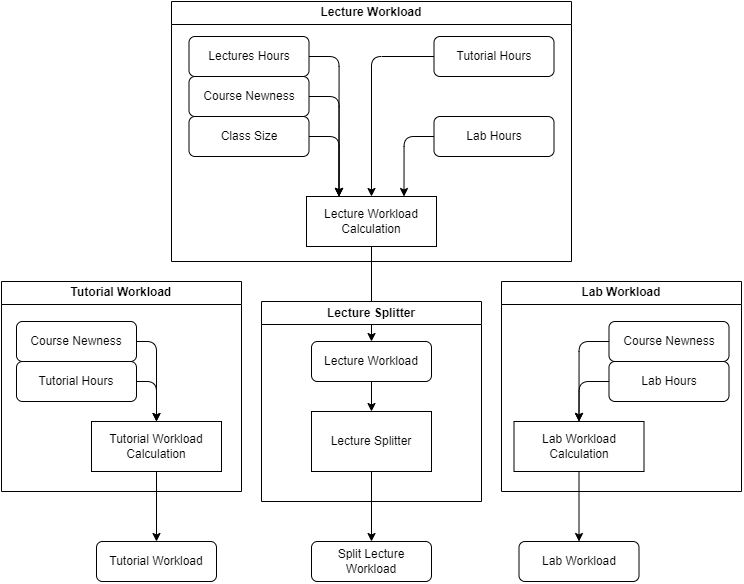
\includegraphics[width=0.9\textwidth]{images/teaching_workload.png}
  \caption{An overview of the teaching workload calculation process}
  \label{fig:teaching-workload}
\end{figure}

\autoref{fig:teaching-workload} shows an overview of the teaching workload calculation process. The workload calculation process is divided lecture, tutorial, and lab workload calculation. The calculated lecture workload further passes through the lecture splitting process to provide the split lecture workload.


\subsection{Demonstration of the model}
\label{sec:workload_demo}

For the purposes of demonstration, we will consider three examples:

\begin{table}[ht]
  \centering
  \begin{tabular}{|l|c|c|c|c|c|}
    \hline
    \textbf{Course}                                  & \(H^{lec}\) & \(H^{tut}\) & \(H^{lab}\) & \(S\) & \(N\) \\\hline
    \(C_1\) - Computer Organisation \& Architecture  & 26          & 13          & 26          & 720   & 0.4   \\\hline
    \(C_2\) - Artificial Intelligence in Game Design & 39          & 0           & 0           & 26    & 0.4   \\\hline
    \(C_3\) - Data Structures                        & 26          & 13          & 26          & 25    & 1     \\\hline
  \end{tabular}
\end{table}

For the above examples, the course workload is shown to be:

\begin{table}[ht]
  \centering
  \begin{tabular}{|l|c|c|c|c|}
    \hline
    \textbf{Course}                                  & \(T_{total}\) & \(T^{lec}\) & \(T^{tut}\) & \(T^{lab}\) \\\hline
    \(C_1\) - Computer Organisation \& Architecture  & 591           & 532         & 23          & 36          \\\hline
    \(C_2\) - Artificial Intelligence in Game Design & 208           & 208         & 0           & 0           \\\hline
    \(C_3\) - Data Structures                        & 493           & 403         & 39          & 52          \\\hline
  \end{tabular}
\end{table}

As you can see, the workload for \(C_1\) is around 3 times the workload of \(C_2\). Most of the difference in workload is accounted for in the lecture workload (\(T_{lec}\)), since the lecture workload is the highest component of the total workload.

You can also see the difference in tutorial and lab workload between \(C_1\) and \(C_3\). This is due to the course newness factor, since \(C_3\) is a new course, while \(C_1\) is an old course. Even with this difference, the tutorial and lab workloads for the two courses are still comparable.

\section{Summary}

\chapter{Faculty Workload Model}

\section{Introduction}

In an academic institution, teaching workload only constitutes a small part of the overall workload of a faculty member. In addition to teaching, faculty members are also expected to perform research, manage staff, acquire research funding, and perform various service activities. The workload of a faculty member is therefore a complex function of the various activities that they perform.

Without equitable distribution of workload, each faculty member would be expected to perform the same amount of work in each of the activities. However, this would be a disservice to the institution as it would not take into account the differences in the abilities of the faculty members, as well as their preferences for the various activities. In addition, the workload of a faculty member is not static, but changes over time as they progress in their career. For example, a lecturers would be expected to spend more time on teaching than research, while a professor would be expected to make significant research and service contributions. Hence, there exists a need for an equitable faculty workload workload which takes the research and service contributions of the faculty members into account.

In the pursuit of an equitable workload distribution, the first step is to quantify the workload of the various activities. This is a non-trivial task as the various activities are not easily quantifiable. The Faculty Workload Model aims to solve this problem by providing a framework for quantifying the workload of the various activities.

\section{Components of Faculty Workload}

A faculty member's workload consists of multiple responsibilities and activities. These responsibilities and activities can be broadly classified into three categories:

\begin{enumerate}
  \item \textbf{Research Workload}

        This refers to the various research activities that the faculty performs. This includes supervision of research staff like post-doctoral fellows and research assistants, contributions towards research publications, acquiring research funding. These activities lead to the creation of new knowledge and the advancement of the research community. The research workload of a faculty member is quantified in \autoref{sec:modelling_research_workload}.

  \item \textbf{Teaching Workload}

        A faculty member's teaching workload consists of the activities that they perform towards the learning of their students. This can further be classified into two categories:

        \begin{enumerate}
          \item Formal Teaching

                This refers to the delivery of lectures, tutorials and labs to the students, and other activities that are directly related to the delivery of the course like preparation of course materials, setting and marking of assignments and examinations, and consultation with students. This part of the teaching workload was described in \autoref{ch:teaching_workload}.

          \item Informal Teaching

                This refers to the supervision of students outside of the formal teaching environment. This includes the supervision of Final-Year Projects (FYPs), Undergraduate Research Experience on Campus (URECA) projects and postgraduate students' research projects.

        \end{enumerate}

  \item \textbf{Service Workload}

        A faculty member's service workload consists of the various service activities that they perform. This includes departmental service - the various service activities that the faculty performs for the department, administrative duties - the various administrative duties that the faculty performs for the institution, and research service duties - the various service activities that the faculty performs for the research community. The service workload of a faculty member is quantified in \autoref{sec:modelling_service_workload}.

\end{enumerate}

\section{Modelling Faculty Workload}

The aim of the faculty workload model is to provide a simplified and accurate picture of the workload of the faculty, providing meaningful insights to the faculty and administration about how the workload of the faculty is distributed across the various activities and how it compares to the workload of other faculty. This is important as the workload of the faculty influences the distribution of teaching workload to the faculty, and the allocation of resources to the various departments. An inaccurate workload allocation model will result in an unfair distribution of workload and resources.

To guide the development of the faculty workload model, a set of objectives and principles were defined. These objectives and principles were used to guide the development of the faculty workload model, and ensure that the faculty workload model is able to achieve its objectives. The faculty workload model was then defined as a set of equations that quantifies the workload of the faculty across the various activities. This allowed the distribution of teaching workload to the faculty to be derived from the workload of the faculty across the various activities.

\subsection{Principles Guiding the Faculty Workload Model}
\label{sec:principles_guiding_workload_allocation_model}

To achieve the objectives of the workload allocation model, it is important to define a set of principles and attributes that the workload allocation model should satisfy. These principles and attributes are:

\begin{enumerate}

  \item \textbf{The workload allocation model should be consistent.}

        The workload allocation model should be able to consistently quantify the workload of various faculty. This is important as the workload allocation model will influence the distribution of teaching workload to the faculty, and the allocation of resources to the various departments. An inaccurate workload allocation model will result in an unfair distribution of workload and resources.

  \item \textbf{The workload allocation model should be transparent and easily understood.}

        Complexity is the enemy of transparency. A complex workload allocation model might be able to accurately quantify the workload of the various activities, but it will be difficult for the faculty to understand how the workload is being allocated. This causes the faculty to lose confidence in the workload allocation model, and will result in a lack of buy-in from the faculty. Additionally, a complex workload allocation model will be difficult to fine-tune and adapt to the needs of the institution.

  \item \textbf{The workload allocation model should be flexible and adaptable to the needs of the institution.}

        Carrying on from the previous point, the workload allocation model should be flexible and adaptable to the needs of the institution. Different institutions have different priorities and needs, and the workload allocation model should be able to adapt to these needs. For example, a teaching-focused institution might want to place more emphasis on teaching workload, while a research-focused institution might want to place more emphasis on research workload. The workload allocation model should be able to adapt to these different needs.

  \item \textbf{The workload allocation model should account for the zero-sum nature of workload.}

        The working hours of a faculty member are finite. As such, the workload of the various activities are zero-sum in nature. For example, a faculty member who spends more time on teaching will have less time to spend on research. The workload allocation model should account for this zero-sum nature of workload. This is important as the workload allocation model will influence the distribution of teaching workload to the faculty, and the allocation of resources to the various departments. An inaccurate workload allocation model will result in an unfair distribution of workload and resources.

  \item \textbf{The workload allocation model should be inclusive and account for the contributions of all faculty members.}

        An academic institution is made up of faculty members of different roles and seniority. The faculty are also broadly classified into lecturers and professors and the institution's goals and priorities for the faculty are influenced by the faculty's role and seniority. For example, a lecturer would be expected to spend more time on teaching than research, while a professor would be expected to make significant research and service contributions. The workload allocation model should be able to account for the contributions of all faculty members, regardless of their roles and seniority.

\end{enumerate}

\subsection{Designing a holistic faculty workload model}

In the absence of overtime, it is fair to assume that the total workload of a faculty should be closely comparable since the faculty are expected to have the same number of working hours, self-allocating any extra time towards research. Thus, the faculty workload model serves greater value in showing the comparative distribution of the workload of various faculty, and the corresponding distribution of their workload across teaching, research and service.

Instead of trying to quantify the workload of the faculty in terms of the number of hours, the ratio of the workload of the faculty across the various activities is quantified. To achieve this, the \textbf{RTS model} for faculty workload was defined as:

\begin{equation*}
  \text{Faculty Workload} = R:T:S
\end{equation*}

where workload of a faculty is represented as a ratio of the workload of the faculty across Research ($R$), Service ($S$) and Teaching ($T$). This model follows the following principles:

\begin{enumerate}
  \item Workload is a zero sum game.

        The sum of the $R$, $T$ and $S$ ratios always adds up to 12. This is because the workload of the faculty is constant, and spending extra time on one activity will result in a reduction of time spent on the other activities. In other words, the workload of the faculty is a zero-sum game.

  \item Linear distribution of workload.

        Each activity is distributed linearly in the model. This means that if a faculty has twice the R-ratio in comparison to another faculty, they are expected to have double the research workload. This is to ensure that the model is easily understandable, and representative of the actual workload of the faculty.

  \item Each Activity has a minimum workload.

        The faculty is allocated a minimum of 2 units of workload for each of the activities. This is to ensure that the faculty are able to make meaningful contributions to the various activities. This also means that each activity has a maximum workload of 8 units, since the sum of the $R$, $T$ and $S$ ratios always adds up to 12.

\end{enumerate}

This RTS model serves not only as a method to quantify the workload of the faculty, but it also serves as a method to distribute the workload. In the scope of this project, since the focus is on the teaching workload of the faculty, the RTS model is used to quantify the research and service workload of the faculty, and accordingly distribute the teaching workload of the faculty as shown in the following sections.


\section{Modelling Research Workload}
\label{sec:modelling_research_workload}

\subsection{Strategies to Quantify Research Workload}

A comprehensive measurement of research workload would require the quantification of the various research activities that the faculty performs. However, the individual research activities are not easily quantifiable. For example, even though we know the number of research papers that the faculty has published, the effort that goes into publishing each research paper can vary greatly depending on the topic of the research paper, the field of study, the quality of the research paper etc. Additionally, measuring at a low level of granularity would result in a large number of error sources, and would also be difficult to fine-tune and adapt to the needs of the institution.

As we we defined in \autoref{sec:principles_guiding_workload_allocation_model}, the workload allocation model should be transparent and easily understood. Thus, a simple and transparent method to quantify the research workload of the faculty is to find an activity that is representative of the entirety of the research workload. This activity should be easily quantifiable, and should be a leading indicator of the research workload of the faculty.


\subsubsection{Research Publication}

Research publication involves performing academic research and publishing the results of the research in conferences and journals. This is one of the most important activities of a faculty member, as it leads to the creation of new knowledge and the advancement of the research community. The workload of research publication is dependent on the number of research papers that the faculty has published, as well as the quality and subject matter of the research papers. For example, a faculty member who has published a research paper in a top-tier conference would generally be expected to have a higher research publication workload than a faculty member who has published a research paper in a lower-tier conference.

However, the research publication workload is difficult to quantify due to the difference in the quality of research, the subject matter of the research papers, as well as the variations in the research publication venues. Moreover, research papers are only published after the research has been completed which makes them a trailing indicator of research publication workload, being able to quantify the research publication workload of the previous semesters, but not the upcoming semester. This makes the research publication workload unsuitable as a measure of the overall research workload of the faculty.

\subsubsection{Research Funding}

Acquiring research funding from external sources involves the writing of research proposals, as well as the application and management of research grants. Different research grants have different levels of complexity and scrutiny in their application process. The research funding may be measured on the basis of the total amount of research funding that the faculty has acquired. The number of research grants that a faculty has acquired or applied to can also be used as a measure of the research funding.

However, this is not an accurate reflection of the total research workload as the amount of research funding that a faculty has acquired as it doesn't directly correlate to the amount of research the faculty has performed. It also doesn't directly correlate to the amount of research staff supervision workload that the faculty has, as the research funding may be used to buy lab equipment, etc. Additionally, research funding is not spent immediately, and may be spent over a period of multiple years. This makes the research funding workload a leading indicator, but the period that the research funding is representative of is not known. Due to these factors, the research funding workload is not suitable as a measure of the overall research workload of the faculty.

\subsubsection{Research Staff Supervision}

Research Staff Supervision refers to the supervision of post-doctoral fellows, research fellows and research assistants. This is one of the most important activities of a faculty member, as most of the research is conducted in collaboration with the research staff that they are supervising. The research staff supervision workload is dependent on the number of research staff that the faculty is supervising, as well as the seniority of the research staff. For example, a faculty member who is supervising a post-doctoral fellow would be expected to spend less time on research supervision than a faculty member who is supervising a research assistant, as the post-doctoral fellow would be expected to be more independent than the research assistant.

The staff supervision workload was found to be a leading indicator of the research publication workload of the faculty. This is because for a faculty, the research is largely conducted in collaboration with the research staff that they are supervising. It is also indicative of the number of future publications that the faculty will be able to author or co-author. Thus, the research staff supervision workload can be used as a proxy for the research publication workload of the faculty. The research publication workload was found to be directly proportional to the research staff supervision workload of the faculty.

Similar to the publication workload, the research funding workload was also found to be directly proportional to the research staff supervision workload of the faculty. This is because the number of research staff that the faculty can hire is dependent on the amount of research funding that the faculty has acquired. Additionally, the assistance of the research staff is also required in the application of research grants. Thus, the research staff supervision workload can be used as a proxy for the research funding workload of the faculty.

The research staff supervision workload was thus found to be a representative indicator of the total research workload of the faculty.

% Additionally, another component of research workload is the research service workload. This includes the service activities that the faculty performs for the research community. For example, the faculty might be serving on the program committee of a conference, or the editorial board of a journal, or might be reviewing research papers for conferences and journals. The workload of research service is dependent on the number of research service activities that the faculty is performing, as well as the seniority of the research service activities. However, this activity is classified as service workload and is not considered as part of the research workload.

\subsection{Calculating Research Workload}
\label{sec:calculating_research_workload}

% Thus, the research workload of a faculty can be written as a function of the research staff supervision workload of the faculty. The research workload of a faculty can be quantified using the following formula:

% \begin{equation*}
%   R = N_{PD} +  N_{RA}
% \end{equation*}

% where $N_{PD}$ is the number of post-doctoral fellows that the faculty is supervising, and $N_{RA}$ is the number of research assistants that the faculty is supervising.

% This has the advantage of being a simple workload allocation model that is easy to understand and fine-tune, as the only parameter that needs to be tuned is the workload of supervising a post-doctoral fellow relative to the workload of supervising a research assistant. Additionally, this is also a leading indicator of the total research workload of the faculty for the upcoming semester.

% \subsection{Addressing Hierarchy Effects in Research}

As described above, quantifying the research workload of a faculty as a function of the research staff working under them has considerable advantages. A simple linear function can be used to quantify the research workload of a faculty. However, one key observation from how faculty supervise a large cohort of research staff was that the faculty do not directly supervise all of the research staff. Instead, the faculty supervise a small number of senior research staff, who in turn supervise a larger number of junior research staff. This not only reduces the workload of the faculty, but also provides a career progression path for the research staff and an opportunity for the senior research staff to gain supervisory experience. To account for this hierarchy effect, a non-linear function can be used to quantify the research workload of a faculty. The non-linear function is expected to have the following properties:

\begin{enumerate}

  \item The research workload of a faculty should be a monotonically increasing function of the number of research staff that they are supervising
  \item The research workload of a faculty should rise linearly for a small number of research staff, and then rise non-linearly for a large number of research staff to account for the hierarchy effect
  \item The research workload of a faculty should asymptotically approach a maximum value as beyond a certain number of research staff, the research workload of the faculty will not increase significantly

\end{enumerate}

The non-linear function that satisfies the above properties is the hyperbolic tangent function, which is defined as:

\begin{equation*}
  \tanh(x) = \frac{e^{2x} - 1}{e^{2x} + 1}
\end{equation*}

where $L$ is the maximum value of the function, $k$ is the steepness of the curve, and $x_0$ is the midpoint of the curve where the function increases linearly. The hyperbolic tangent function is plotted in \autoref{fig:tanh_full_function}.

\begin{figure}[htpb]
  \centering
  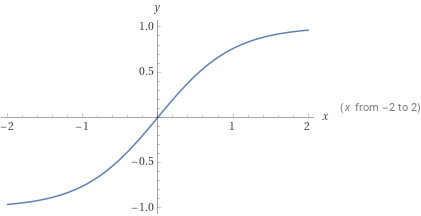
\includegraphics[width=0.5\linewidth]{images/tanh_fullplot.png}
  \caption{\(\tanh(x)\) for \(x \in [-2, 2]\)}
  \label{fig:tanh_full_function}
\end{figure}

We're only interested in the positive half of the hyperbolic tangent function, which has a constant slope for $x \to 0$, and is asymptotic to 1 as $x \to \infty$. The positive half of the hyperbolic tangent function is plotted in \autoref{fig:tanh_function}.

\begin{figure}[htpb]
  \centering
  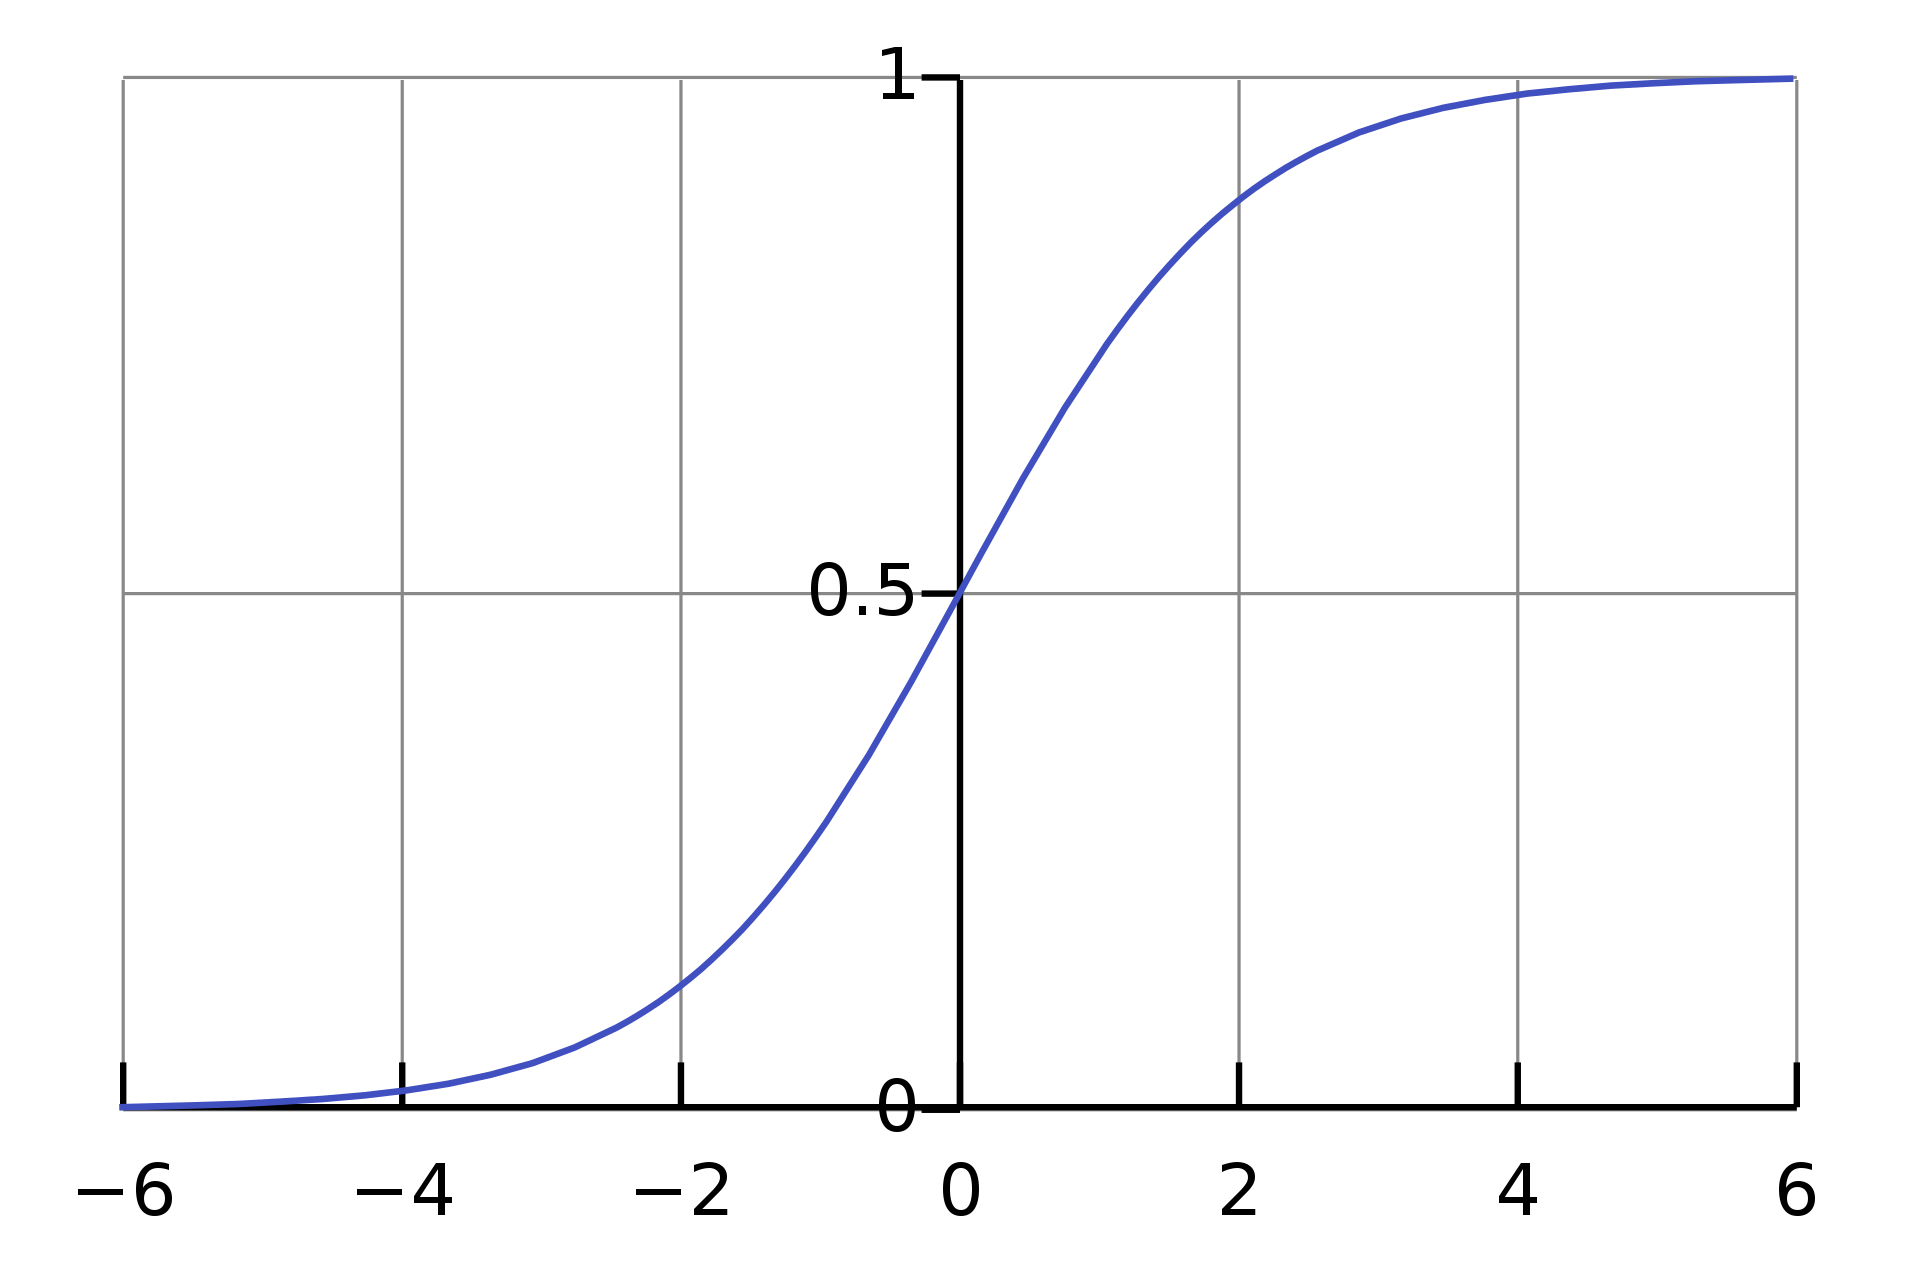
\includegraphics[width=0.5\linewidth]{images/tanh_plot.png}
  \caption{\(\tanh(x)\) for \(x \in [0, 4]\)}
  \label{fig:tanh_function}
\end{figure}


It was found that due to the hierarchical nature of research staff management, the research staff supervision workload can be modelled using a hyperbolic tangent function has a range of $[0, 1]$. Since it is known that the range of the research workload is between 2 and 8, i.e. a range of 6 units, the research workload is rescaled to have a range of $[2, 8]$. The steepness of the curve was also tweaked so that the research workload so that the research workload approaches the maxima at around 10 research staff. This results in the following formula:

\begin{equation}
  R  = 2 + 6\ \tanh(x/6)
\end{equation}

where $x$ is the total number of research staff members that the faculty is supervising. Individual research staff seniority was not taken into account, since the hiring patterns of the faculty are such that a small number of senior research staff are hired, who in turn supervise a larger number of junior research staff.

\begin{figure}[H]
  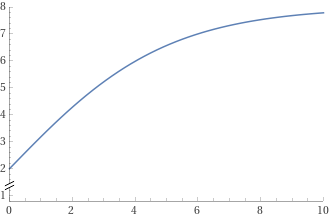
\includegraphics[width=0.5\textwidth]{images/rts_research_plot.png}
  \centering
  \caption{Research Workload ($R$)}
  \label{fig:rts_research_plot}
\end{figure}

\autoref{fig:rts_research_plot} shows the research workload of the faculty as a function of the number of research staff that the faculty is supervising. The research workload is a monotonically increasing function of the number of research staff that the faculty is supervising. The research workload rises linearly for a small number of research staff, and then rises non-linearly for a large number of research staff to account for the hierarchy effect. The research workload asymptotically approaches a maximum value of 8 as beyond a certain number of research staff, the research workload will not increase significantly.


\section{Modelling Service Workload}
\label{sec:modelling_service_workload}

The service workload of a faculty consists of the various service activities that they perform. The service activities of a faculty include but are not limited to the following:

\begin{enumerate}

  \item \textbf{Departmental Service}

        This is the various service activities that the faculty performs for the department. It includes serving on departmental committees, as well as performing administrative duties for the department.

  \item \textbf{Administrative Duties}

        This is the various administrative duties that the faculty performs for the institution. It includes duties like serving on various committees and panels the admissions panel, the scholarship review panel and the examinations committee, coordinating a research center etc.

  \item \textbf{Research Service Duties}

        This is the various service activities that the faculty performs for the research community. It includes serving on the program committee of a conference, or the editorial board of a journal, or reviewing research papers for conferences and journals.

\end{enumerate}

The service workload of a faculty is dependent on the number of service duties that the faculty is performing, as well as the amount of effort required to perform each of these duties. Since the nature of each service duty is different, it is difficult to quantify the service workload of a faculty through a heuristic approach. Instead, a simple weighted average of the service workload of each of these duties can be used, where the weights correspond to the workload per semester for each of these duties. The service workload of a faculty can be quantified using the following formula:

\begin{equation*}
  \text{Service Workload} = \sum_{i=1}^{N_{sd}} w_i
\end{equation*}

where $N_{sd}$ is the number of service duties that the faculty is performing, and $w_i$ is the workload per semester of the $i$-th service duty.

Some of the service duties are performed by all faculty members. For example, all faculty members are expected to perform some research service duties, be it reviewing research papers or serving on the program committee of a conference. These service duties are excluded from the workload allocation model as they are not indicative of the workload of an individual faculty member. The allocation of service duties also depends on the seniority of the faculty member. For example, a junior faculty member would be expected to generally perform less service duties and contribute primarily towards teaching and research, while as the faculty member progresses in their career, they would be expected to perform more service duties like serving on departmental committees and major administrative duties like coordinating a research center, or even serving as the Chair of the department. A typical faculty member would be expected to perform 0-2 service duties per semester, while senior faculty members would be expected to perform 2-4 service duties per semester.

Some of the service duties and their corresponding workload per semester are shown in \autoref{tab:service_duties}.

\begin{table}[htpb]
  \centering
  \begin{tabular}{|l | l | r |}
    \hline
    Designation     & Service Duty                                  & Workload \\
    \hline
    Member          & Industrial Attachment Steering Committee      & 1.00     \\
    Member          & Research Mentorship and Consultancy Committee & 1.00     \\
    Member          & Nanyang Research Programme Committee          & 1.00     \\
    Coordinator     & Final Year Projects                           & 1.00     \\
    Director        & Research Centre                               & 1.00     \\
    Group Lead      & Research Focus Group                          & 1.25     \\
    Member          & Research Integrity Committee                  & 1.00     \\
    Member          & Scholarship Interview Panel                   & 1.00     \\
    Member          & School Review Committee                       & 1.00     \\
    Member          & School Reappointment Committee                & 1.00     \\
    Member          & School Search Committee                       & 1.00     \\
    Chairperson     & Student Outreach Committee                    & 1.25     \\
    Coordinator     & Time-Tabling                                  & 1.00     \\
    Associate Chair & Associate Chair                               & 1.00     \\
    \hline
  \end{tabular}
  \caption{An example of how service duties and workload can be framed}
  \label{tab:service_duties}
\end{table}


It was found that each of the service duties has a particular impact on the workload of the faculty. For example, serving on the Industrial Attachment Steering Committee has an impact of 1 unit. In addition, even if the faculty is not performing any service duties, they are still expected to perform a minimum of 2 units of service workload. Thus, the service workload of the faculty can be quantified using the following formula:

\begin{equation}
  S = 2 + \sum_{i=1}^{N_{sd}} w_i
\end{equation}

where $N_{sd}$ is the number of service duties that the faculty is performing, and $w_i$ is the workload per semester of the $i$-th service duty.

A maximum cap of 8 units is also imposed on the service workload of the faculty, since the sum of the $R$, $T$ and $S$ ratios always adds up to 12. This means that a faculty will only be rewarded for their service duties up to a certain extent. This is to ensure that the faculty are able to make meaningful research and teaching contributions as well, and not be overloaded with service duties.

\section{Determining Equitable Teaching Workload}

The service and research workload of the faculty are predictive, i.e. they are leading indicators of the workload of the faculty for the upcoming semester. The number of staff that the faculty is supervising is indicative of how much research workload will be involved, and the number of service duties that the faculty is performing for the semester is indicative of how much service workload will be involved.

While the research and service workload are pre-determined, we have the opportunity to use the teaching workload to balance the workload of the faculty. This allows the total workload of each faculty to be comparable, and ensures that the faculty are not overloaded with work. Thus, with the service and research workload of the faculty quantified, the teaching workload of the faculty can be derived from the RTS model. Since $R + T + S = 12$, the teaching workload of the faculty can be quantified using:

\begin{equation}
  T = 12 - R - S
\end{equation}

The teaching workload is also subject to the same minimum and maximum workload constraints as the research and service workload. This means that the teaching workload of the faculty is capped at a maximum of 8 units, and a minimum of 2 units. This is to ensure that the school is able to make use of their teaching expertise in their respective fields.


\begin{figure}[H]
  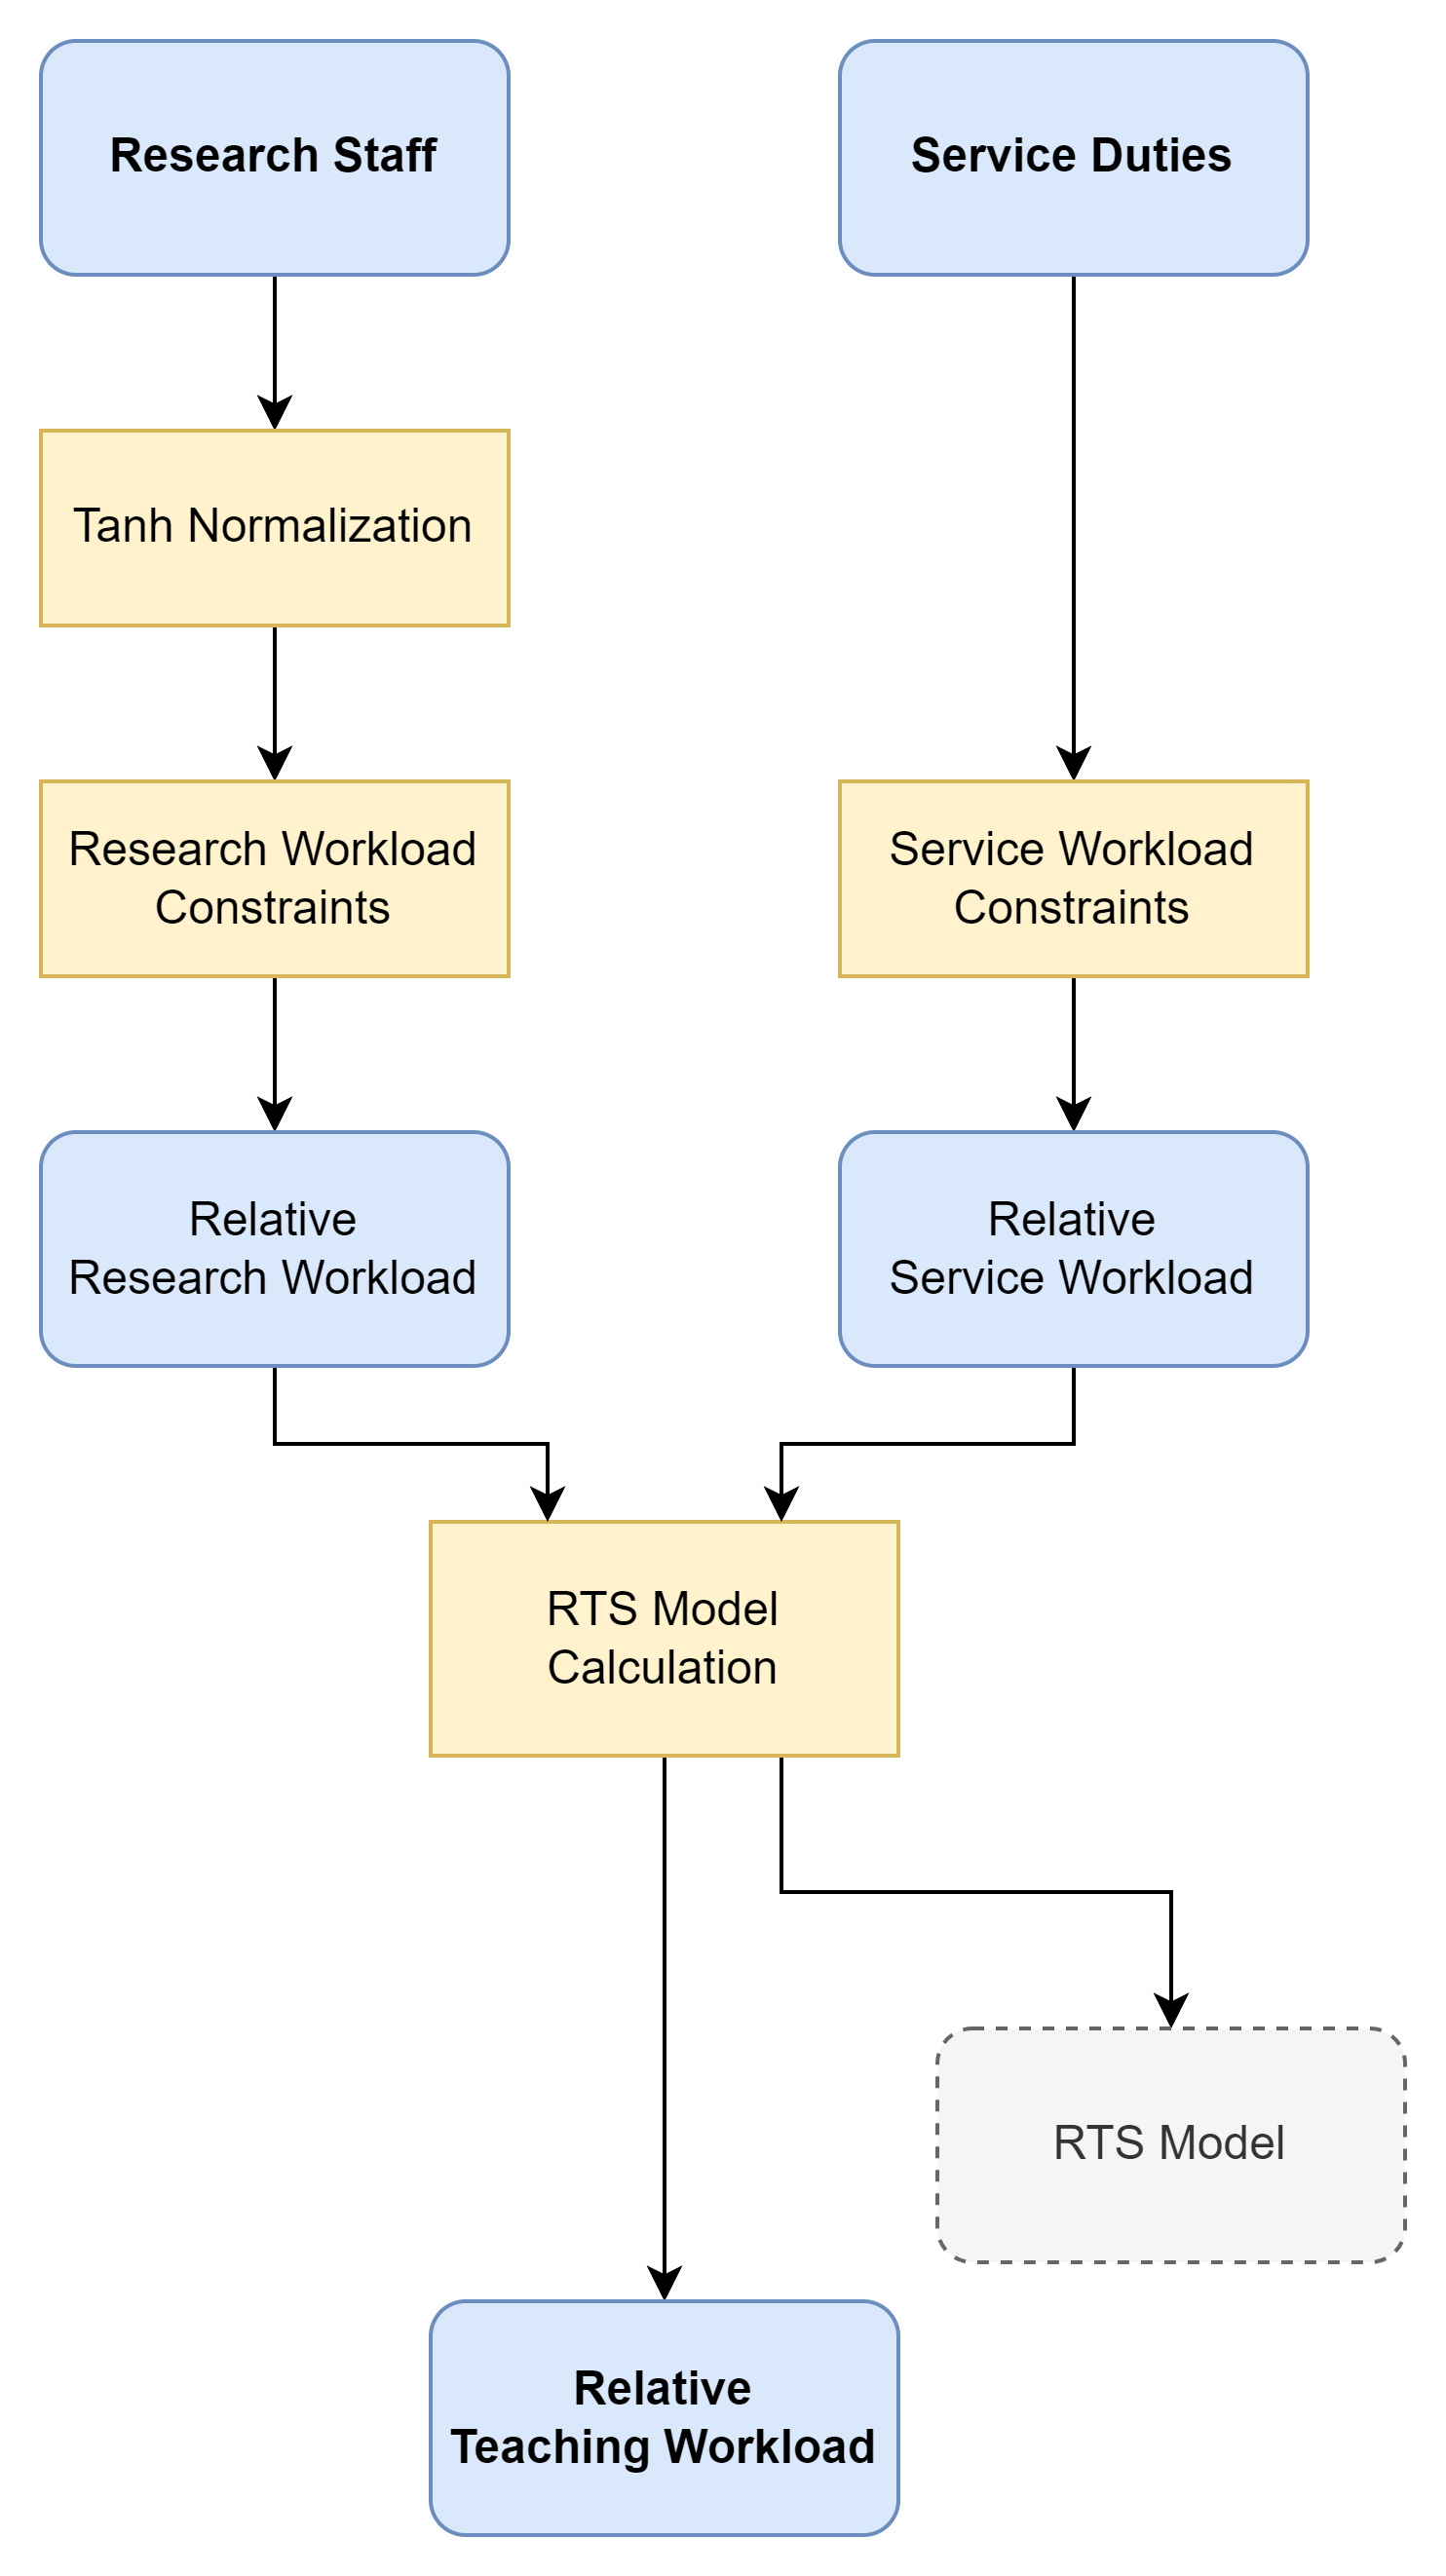
\includegraphics[width=0.5\textwidth]{images/faculty_wam.png}
  \centering
  \caption{Deriving Teaching Workload from RTS Model}
  \label{fig:faculty_wam}
\end{figure}


\section{Summary}

The RTS Model for faculty workload establishes a simple and transparent method to quantify and distributing the faculty workload in an equitable manner. This involves quantifying the research workload of the faculty as a function of the number of research staff that the faculty is supervising, and quantifying the service workload of the faculty as simple weighted increments for each of the service duties that the faculty is performing. This allows the teaching workload of the faculty to be derived from the RTS model, and ensures that the total workload of each faculty is comparable.

In the next chapter, the teaching workload derived using the RTS model will be used as the basis for the lecture allocation problem, where it will establish the limits for the teaching workload of the faculty to ensure that the faculty are not overloaded with work.


\chapter{Lecture Allocation}

\section{Introduction}

The goal of the lecture allocation problem is to allocate the lectures of each course to the faculty members who are teaching the course in a way that ensures the students have a good learning experience and the faculty members are not overworked. The previous chapters have defined the amount of work involved in each activity of the teaching workload, as well as the amount of workload that each faculty member can handle. The lecture allocation process should take these factors into account when allocating the lectures of each course to the faculty members who are teaching the course. Additionally, it should also incorporate the preferences of the faculty members and the management.

In this chapter, the lecture allocation problem will be defined and modelled as a multi-constraint optimization problem which can be solved using the Hungarian algorithm. To solve this, a course-faculty fit metric will be defined to determine the suitability of a faculty member to teach a course in regards to the student learning experience and the faculty preferences. The course-faculty fit metric will be used to define the objective function of the optimization problem. The lecture allocation problem will be solved using the Hungarian algorithm and the results will be analysed on the basis of optimality and scalability. The constraints of the optimization problem will be defined to ensure that the workload limits of the faculty members are not exceeded and the preferences of the faculty members and the management are taken into account. Various strategies will also be proposed to improve the quality of the allocation results.

\section{Ensuring Course-Faculty Fit}

The first step towards solving the allocation problem is defining what makes a faculty member suitable to teach a course. This should incorporate the priorities of the students, the management, and the faculty members. Additionally, it should also be easy to understand and explain, easy to collect the data required to compute it, and easy to compute. It should also be easy to tweak and improve, since the priorities of different institutions may be different.



\subsection{Student Feedback}

The students are the most important stakeholders in the decision of which faculty member should teach a course, since their learning experience and outcomes are directly affected by this decision. Their priorities are to be taught by a faculty member who is experienced at teaching and knowledgeable about the subject matter. This priority can be quantified by collecting the feedback of the students about the faculty member who taught the course in the past.

At the end of a semester, the student feedback is collected on their learning experience in the courses they were taught. This feedback is collected in the form of a survey, which is filled by the students and submitted to the management. The survey contains questions about the faculty members who taught the course, the course content, the pace of the course and the overall learning experience. The feedback is collected for each course and faculty member combination. This feedback may also be collected periodically during the semester, especially for courses that are taught in multiple parts by different faculty members.

Peer feedback is also collected from the faculty members of the department, which is used to evaluate the teaching skills of the faculty members. This includes questions about the teaching skills of the faculty members, and their knowledge of the subject matter.

These feedback components are then combined into a \textbf{Student Feedback Score} for each course-faculty combination, which is a number between 0 to 5. This score is calculated by taking a weighted average of the student feedback and the peer feedback, with student feedback being weighted more than the peer feedback, since the student feedback is more representative of the learning experience of the students.

Since there are also faculty who are eligible to teach a course, but have never taught the course before, they will not have any student feedback. In this case, the peer feedback is combined with the average student feedback for the course to calculate the Student Feedback Score.

\subsection{Faculty Preference}

With manual allocation, faculty members are often left with no choice in the courses they teach. The largely static allocation process leaves faculty members with similar teaching assignments every semester, which may lead to a lack of motivation and interest in teaching. With the automated allocation process, faculty members can be given the opportunity to teach courses that they are interested in, which will lead to a better learning experience for the students and a better teaching experience for the faculty members.

Before every semester, the faculty are asked to submit their preferences for the courses they would like to teach. This is done by asking the faculty members to rank the courses they are eligible to teach in the order of their preference. They are required to rank every course that they are eligible to teach, which also forms the basis for a course-eligibility criteria, since they should not be given courses that are completely out of their area of expertise. Additionally, the courses they have taught in the past are also treated as eligible courses, even if they are not directly ranked by the faculty. The management requires the faculty to provide a minimum number of preferences to ensure that courses are not left unallocated.

These preference scores are then normalized to a number between 0 to 5 to form the \textbf{Faculty Preference Score} for each course-faculty combination. This score is calculated by taking the list of preferences provided by the faculty and linearly distributing it between 0 to 5, such that the first preference is given a score of 5, the tenth preference is given a score of 0. The preferences for courses beyond the tenth preference are given a score of 0. The courses that are not ranked by the faculty are also given a score of 0.

\subsection{Management Priorities}

The management priority is to ensure the long-term learning path of the students is optimal throughout the duration of the program. This means establishing a strong foundation for the students in the early years of their program, and then building on that foundation in the later years. This is done by ensuring that the courses in the early years of the degree are taught by highly experienced faculty members with a good teaching performance score. The latter year courses on the other hand can be allocated with a higher priority to the faculty members who are more interested in teaching the course, since this is reflective of the faculty's research interests, which makes them more knowledgeable about the subject matter for the advanced courses in the program.

This can be achieved by ensuring that the higher year courses are given a priority to be taught by the faculty members with the best ratings. This prioritization can be done in an absolute manner, where the courses are allocated in the sequence of their year of study, thus ensuring that the courses in the earlier years can reserve the best faculty members. This can also be done in a soft manner, biasing the allocation of earlier year courses towards the best faculty members by manipulating the course-faculty fit metric. This will be discussed in detail in the next section.

\section{Defining The Allocation Problem}

The lecture allocation involves allocating the lectures of each course to the faculty members who are teaching the course. It can be defined as a constrained multi-objective optimization problem, with a set of objectives that need to be optimized and a set of constraints that need to be satisfied.

The primary objective of the allocation problem is to ensure that all the courses are allocated to the faculty members, since unallocated courses will lead to cancellation of the course. Additionally, the allocation problem should also ensure that the workload of the faculty members is distributed equitably, and they receive a similar workload in terms of lectures, tutorials and practicals. The allocation problem should also ensure that the earlier year courses are taught by the best faculty as per the management priorities. Finally, the allocation problem should ensure that the faculty members are allocated the courses that they are interested in teaching, which will lead to a better teaching experience for the faculty members. These objectives are described in detail in the following sections.

\begin{enumerate}
  \item \textbf{Ensure all courses are allocated}

        The allocation problem should ensure that all the courses are allocated to a faculty member. This is a hard constraint of the allocation problem, since unallocated courses will lead to cancellation of the course, which will adversely impact the learning experience of the students, and may impact their long-term learning path since some courses may form a prerequisite for other courses.

        There are some prerequisites to this constraint - the allocation process cannot allocate a course if there are no eligible faculty members to teach the course, or if the maximum workload for the faculty members is already reached. However, given that these prerequisites are met, the allocation process should ensure that all the courses are allocated.

  \item \textbf{Distribute workload in proportion to the relative teaching workload}

        The relative teaching workload, defined in the previous chapter, is a measure of the amount of teaching workload that a faculty member can handle, relative to the other faculty members. Thus, distributing the workload in proportion to the relative teaching workload ensures that teaching workload is distributed equitably among the faculty members, ensuring that no faculty member is overworked.

  \item \textbf{Distribute a similar proportion of lectures, tutorials and practicals to each faculty member}

        A course consists of multiple teaching activities, such as lectures, tutorials, and practicals. Preferably, these teaching activities should be distributed equally among the faculty members, so that each faculty member has a similar teaching experience. This is a soft constraint of the allocation problem, since it is not as important as the other objectives, but it is still desirable to have a balanced teaching experience for the faculty members.

  \item \textbf{Ensure that earlier year courses are taught by the best faculty members}

        The management priority is to ensure that the earlier year courses are taught by the faculty members with the best ratings since this is the foundation for the students' learning path. This means that the earlier year courses should be allocated with a higher priority to the faculty members with the best ratings. This is a soft constraint of the allocation problem, since it is not as important as the other objectives, but it is still desirable to have the earlier year courses taught by the best faculty members.

  \item \textbf{Maximize the faculty performance score}

        The faculty performance score, defined in the previous section, is a measure of the suitability of a faculty member to teach a course. It is representative of the student learning experience, and thus, maximizing the total faculty performance score of the allocation ensures that the students have a good learning experience. This is the primary objective of the allocation problem.

  \item \textbf{Maximize the faculty preference score}

        The faculty preference score, defined in the previous section, is a measure of the preference of the faculty member to teach a course. Thus, maximizing the total faculty preference score of the allocation ensures that the faculty members are allocated the courses that they are interested in teaching, which will lead to a better teaching experience for the faculty members.

        This is treated as a secondary objective of the allocation problem, since it is not as important as the primary objective of maximizing the faculty performance score. However, given that the faculty performance score is comparable between two allocations, the allocation with the higher faculty preference score is preferred.


\end{enumerate}

\section{Modelling The Allocation Problem}

The lecture allocation problem can be modelled as an assignment problem, where the tasks are the lectures of each course, and the agents are the faculty members who are teaching the course. Each lecture's assignment to a faculty member should have a cost that represents the objectives of the allocation problem. Every lecture of a course must be assigned to exactly one faculty member, while each faculty member may be assigned to multiple lectures of multiple courses.

The cost of assigning a course to a faculty member should represent the suitability of the faculty member to teach the course by taking into account the student feedback. It should also represent the preference of the faculty member to teach the course by using the faculty preference rankings provided by the faculty members. Additionally, allocation of low cost faculty members to earlier year courses should be prioritized to ensure that the earlier year courses are taught by the best faculty members.

It also needs to be ensured that the workload is distributed among the faculty members in proportion to their relative teaching workload, which was defined in the previous chapter. This proportionality is achieved by ensuring that the workload of the faculty members does not exceed their workload limits, where the workload limits are defined proportional to the faculty's relative teaching workload.

In the next section, we will define how this constrained cost-minimization problem can be solved using the Hungarian algorithm.

\subsection{The Hungarian Algorithm}

The Hungarian Algorithm, also known as the Kuhn-Munkres Algorithm, is a combinatorial optimization algorithm that solves the assignment problem in polynomial time. In comparison to other algorithms that solve the assignment problem, such as the genetic algorithm and the simulated annealing algorithm, the Hungarian algorithm is faster and more efficient, and is more deterministic in nature. This makes it a good choice for solving the lecture allocation problem, since the faculty, students and management expect the allocation to be deterministic.

The Hungarian algorithm solves the assignment problem by finding the optimal assignment between the tasks and the agents, where each task is assigned to exactly one agent, and each agent is assigned to exactly one task. The optimal assignment is the one that minimizes the total cost of assigning the tasks to the agents. For an unequal number of tasks and agents, the Hungarian algorithm can be used to find the optimal assignment by adding dummy tasks or dummy agents, which are assigned a cost of 0. This ensures that the total cost of the assignment is not affected by the dummy tasks or dummy agents. This also means that for more tasks than agents, some of the tasks will be left unassigned.

However, a university typically has more lectures than the number of faculty members, which means that each faculty member will have to teach multiple lectures of a course. Thus, the allocation problem is split into multiple iterations of the Hungarian algorithm, where each iteration allocates one lecture of each course to a faculty member.

The cost matrix for the Hungarian algorithm is constructed by calculating the cost of assigning each course to each faculty member. The cost of assigning a course to a faculty member is calculated by taking the course-faculty fit metric, and subtracting it from 5. This is done to ensure that the cost of assigning a course to a faculty member is inversely proportional to the course-faculty fit metric, since the Hungarian algorithm minimizes the total cost of the assignment. The cost matrix is constructed using the algorithm shown in \autoref{alg:cost_matrix_construction}.

\begin{algorithm}[H]
  \caption{Cost Matrix Construction for Lecture Allocation}
  \begin{algorithmic}[1]
    \Procedure{ConstructMatrix}{$lectures$, $faculty$}
    \For{$l \in lectures$}
    \For{$f \in faculty$}
    \If{$f \text{ can teach } l$}
    \State $cost \gets Q(l, f)$
    \Else
    \State $cost \gets \infty$
    \EndIf
    \State $costMatrix[l][f] \gets cost$
    \EndFor
    \EndFor
    \EndProcedure
  \end{algorithmic}
  \label{alg:cost_matrix_construction}
\end{algorithm}

where, \(lectures\) is the list of lectures of each course, \(faculty\) is the list of faculty members, and \(Q(l, f)\) is the cost function for assigning course lecture \(l\) to faculty member \(f\).

With the cost matrix constructed, the Hungarian algorithm can be used to allocate the lectures of each course to the faculty members who are teaching the course. The allocation process is split into multiple iterations of the Hungarian algorithm, where each iteration allocates one lecture of each course to a faculty member.

In each iteration of the loop, we use \autoref{alg:cost_matrix_construction} to construct the cost matrix, and then use the Hungarian algorithm to find the optimal assignment between the courses and the faculty members. Some of these assignments may be dummy assignments which are created due to the unequal number of courses and faculty members. These dummy assignments are ignored, and the remaining assignments are added to the list of all assignments. We run this loop until either all the lectures are allocated. However, if no new lectures are allocated in an iteration, then the loop is broken, since no progress is being made. This is shown in \autoref{alg:base_lec_alloc}.

\begin{algorithm}[H]
  \caption{Lecture Allocation Algorithm}
  \begin{algorithmic}[1]
    \Procedure{AllocateLectures}{$lectures$, $faculty$}
    \State $unallocatedLectures \gets lectures$
    \State $allocatedLectures \gets \emptyset$
    \State $allAssignments \gets \emptyset$
    \While {$unallocatedLectures \neq \emptyset$} \Comment{Iterate until all lectures are allocated}
    \State $costMatrix \gets \text{ConstructMatrix}(unallocatedLectures, faculty)$
    \State $assignments \gets \text{HungarianAlgorithm}(costMatrix)$
    \State $assignedCount \gets 0$
    \For {$assignment \in assignments$}
    \If {$assignment \text{ is not a dummy assignment}$}
    \State $allAssignments \gets allAssignments \cup assignment$
    \State $allocatedLectures \gets allocatedLectures \cup assignment$
    \State $unallocatedLectures \gets unallocatedLectures \setminus assignment$
    \State $assignedCount \gets assignedCount + 1$
    \EndIf
    \EndFor
    \If {$assignedCount = 0$}
    \State \textbf{Break Loop}
    \Comment{if no new lectures allocated, break the loop}
    \EndIf
    \EndWhile
    \State \Return $allAssignments$
    \EndProcedure
  \end{algorithmic}
  \label{alg:base_lec_alloc}
\end{algorithm}

where, \(lectures\) is the list of lectures of each course, \(faculty\) is the list of faculty members, \(unallocatedLectures\) is the list of lectures that are yet to be allocated, \(allocatedLectures\) is the list of lectures that are already allocated, and \(allAssignments\) is the list of all the assignments made by the Hungarian algorithm.

This lecture allocation algorithm $AllocateLectures$ forms the basis for the lecture allocation process in the latter stages, and is used as the building block for the various strategies proposed in the following sections. It involves multiple iterations of the Hungarian algorithm, where each iteration allocates one lecture of each course to a faculty member.

The Hungarian algorithm is run in each iteration until all the lectures are allocated. The assignments made by the Hungarian algorithm are then added to the list of all assignments, and the allocated lectures are removed from the list of unallocated lectures. This process is repeated until all the lectures are allocated.

\subsection{Enforcing Workload Limits}

With the lecture allocation algorithm defined in \autoref{alg:base_lec_alloc}, the lectures of each course are allocated to the faculty members who are teaching the course. However, this allocation does not take into account the existing workload of the faculty members, which may lead to disproportionate allocation of workload. To counter this, the allocation algorithm is modified to enforce the workload limits of the faculty members.

To enforce the workload limits, we first define the workload limits of the faculty members using the relative teaching workload, which was defined in the previous chapter. Then we incorporate the workload limits into the lecture allocation algorithm by modifying the cost matrix construction algorithm to ensure that the workload of the faculty members does not exceed their workload limits.

\subsubsection{Defining the Workload Limits}

The workload limits of the faculty members are previously defined in \autoref{sec:determining_equitable_teaching_workload} as the relative teaching workload. The relative teaching workload is a measure of the amount of teaching workload that a faculty member can handle, relative to the other faculty members. However, the workload of the faculty members is defined in terms of workload units, while the workload limits are defined relative to the other faculty members. Thus, the workload limits need to be converted to workload units to be enforced.

To convert the workload limits to workload units, the total workload units of the department are calculated, which is the sum of the workload units of all the courses. The workload limits of the faculty members are then converted to workload units by multiplying the workload limits with the total workload units of the department and dividing it by the total number of relative workload units of the faculty members. This is shown in \autoref{eq:workload_limits}.

\begin{equation}
  \label{eq:workload_limits}
  \begin{aligned}
    T_{total} & = \sum_{c \in courses} T_c               \\
    R_{total} & = \sum_{f \in faculty} R_f               \\
    T_f       & = R_f \times \frac{T_{total}}{R_{total}}
  \end{aligned}
\end{equation}

where,
\begin{align*}
  T_{total} & = \text{Total workload units of the department}               \\
  T_c       & = \text{Workload units of the course } c                      \\
  R_{total} & = \text{Total relative workload units of the faculty members} \\
  R_f       & = \text{Relative workload units of the faculty member } f     \\
  T_f       & = \text{Workload units limit of the faculty member } f
\end{align*}

\subsubsection{Lecture Allocation with Workload Limits}

With the workload limits of the faculty members defined in terms of workload units, the lecture allocation algorithm is modified to enforce the workload limits of the faculty members. This is done by ensuring that the workload of the faculty members does not exceed their workload limits at the time of cost matrix construction. This is shown in \autoref{alg:workload_limit_cost_matrix_construction}.

\begin{algorithm}[H]
  \caption{Cost Matrix Construction with Workload Limits}
  \begin{algorithmic}[1]
    \Procedure{ConstructMatrixWithWorkloadLimits}{}
    \For{$l \in lectures$}
    \For{$f \in faculty$}
    \If{($f \text{ can teach } l) \text{ and } (existingWorkload[f] + T[l]$ \textless $workloadLimits[f]$)}
    \State $cost \gets 5 - Q(l, f)$
    \Else
    \State $cost \gets \infty$
    \EndIf
    \State $costMatrix[l][f] \gets cost$
    \EndFor
    \EndFor
    \Return $costMatrix$
    \EndProcedure
  \end{algorithmic}
  \label{alg:workload_limit_cost_matrix_construction}
\end{algorithm}

where, \(lectures\) is the list of lectures of each course, \(faculty\) is the list of faculty members, \(existingWorkload\) is the already allocated workload of the faculty members, \(T[l]\) is the workload units of the lecture \(l\), and \(workloadLimits\) is the workload limits of the faculty members.

By using this modified cost matrix construction algorithm, the workload limits of the faculty members are enforced every time the Hungarian algorithm is run. This ensures that the workload of the faculty members are ineligible to teach a course if their workload exceeds their workload limits.

\subsection{Handling Management Priority}

The management priority is to ensure that the earlier year courses are taught by the faculty members with the best ratings since this is the foundation for the students' learning path. This means that the earlier year courses should be allocated with a higher priority to the faculty members with the best ratings.

Since the faculty has a finite workload limit, as defined in the previous section, the faculty members with the best ratings have to be allocated to the earlier year courses first, since the courses which are allocated first might fulfil the workload limits of the faculty members, thus making them ineligible to teach any courses that are allocated later. This is especially true for the faculty members with a low workload limit, since they can only teach a few courses, and thus, they have to be allocated to the earlier year courses first.

To achieve this, the courses are allocated in the sequence of their year of study, thus ensuring that the courses in the earlier years can reserve the best faculty members. This is done by iterating over the courses in the order of their year of study, and allocating the courses in that order. This ensures that the courses in the earlier years are allocated first, and thus, they can reserve the best faculty members, meeting the hard constraint of the management priority.

The lecture allocation algorithm is modified to incorporate this approach by filtering the list of courses to be allocated by the year of study, then iterating over the filtered list of courses year-wise, and allocating the courses in that order. This is shown in \autoref{alg:year_wise_lec_alloc}.

\begin{algorithm}[H]
  \caption{Year-wise Lecture Allocation Algorithm}
  \begin{algorithmic}[1]
    \Procedure{AllocateLecturesYearwise}{$lectures$, $faculty$}
    \State $allAssignments \gets \emptyset$
    \For{$year \gets 1$ to $maxYear$} \Comment{Iterate over the years}
    \State $yearLectures \gets \text{FilterByYear}(lectures, year)$
    \State $yearAllocations \gets AllocateLecturesWithWorkloadLimits(yearLectures, faculty)$
    \State $allAssignments \gets allAssignments \cup yearAllocations$
    \EndFor
    \State \Return $allAssignments$
    \EndProcedure
  \end{algorithmic}
  \label{alg:year_wise_lec_alloc}
\end{algorithm}

where, $AllocateLecturesWithWorkloadLimits$ is the lecture allocation algorithm defined in \autoref{alg:base_lec_alloc}, but using the cost matrix construction algorithm that uses the faculty workload limits, as defined in \autoref{alg:workload_limit_cost_matrix_construction}.

% \subsection{Soft Priority}

% In this approach, the courses are allocated in a soft manner, biasing the allocation of earlier year courses towards the best faculty members by manipulating the course-faculty fit metric. This is done by reducing the cost of assigning a course to a well rated faculty members and increasing the cost of low rated faculty members in earlier years courses.

% This bias factor that is introduced in the course-faculty fit metric is kept as a configurable parameter, which is higher for the earlier year courses and lower for the later year courses. This ensures that the earlier year courses are allocated with a higher priority to the faculty members with the best ratings, while the later year courses are allocated with a lower priority to the faculty members with the best ratings. The biases used for the different years are shown in Table \autoref{tab:year_wise_bias}.

% \begin{table}[H]
%   \centering
%   \begin{tabular}{|c|c|c|c|c|c|}
%     \hline
%     \textbf{Year} & \textbf{1} & \textbf{2} & \textbf{3} & \textbf{4} & \textbf{5} \\ \hline
%     \textbf{Bias} & 1          & 0.75       & 0.5        & 0.25       & 0          \\ \hline
%   \end{tabular}
%   \caption{Year-wise Bias}
%   \label{tab:year_wise_bias}
% \end{table}

% Additionally, the best faculty members need to be defined, which is done by defining a threshold Teaching Performance Score. The faculty members with a Teaching Performance Score above the threshold are considered to be the best faculty members. This threshold is kept as a configurable parameter, which can be tweaked to suit the priorities of the institution. As a default, the threshold Teaching Performance Score is kept as 4.5, which filters out the top performing faculty members  from the rest.

% With the biases and the threshold Teaching Performance Score defined, the cost matrix calculation algorithm is modified to incorporate the soft priority approach. This is shown in \autoref{alg:soft_priority_cost_matrix_construction}.

% \begin{algorithm}[H]
%   \caption{Soft Priority: Biased Cost Matrix Construction}
%   \begin{algorithmic}[1]
%     \Procedure{ConstructBiasMatrix}{$lectures$, $faculty$}
%     \For{$l \in lectures$}
%     \For{$f \in faculty$}
%     \If{$f \text{ can teach } l$}
%     \State $fitScore \gets Q(l, f)$
%     \If{$fitScore \geq threshold$} \Comment{if faculty is one of the best faculty members}
%     % sum of cost and bias
%     \State $cost \gets cost - getBias(l.year)$
%     \Else
%     \State $cost \gets cost + getBias(l.year)$
%     \EndIf
%     \Else
%     \State $cost \gets \infty$
%     \EndIf
%     \State $costMatrix[l][f] \gets cost$
%     \EndFor
%     \EndFor
%     \EndProcedure
%   \end{algorithmic}
%   \label{alg:soft_priority_cost_matrix_construction}
% \end{algorithm}

\subsection{Defining the Cost Function (\(Q\))}
\label{sec:defining_the_cost_function}

To solve the lecture allocation problem using the Hungarian algorithm, a cost function \(Q\) needs to be defined, which represents the suitability of a faculty member to teach a course. This cost function is used to calculate the cost of assigning a course to a faculty member, which is used by the Hungarian algorithm to find the optimal assignment between the courses and the faculty members.

To define the cost function, we first define a course-faculty fit metric. This course-faculty fit metric is a number between 0 to 5 that represents the suitability of a faculty member to teach a course. This metric is calculated by taking a weighted average of the Student Feedback Score and the Faculty Preference Score, with the Student Feedback Score being weighted more than the Faculty Preference Score. This is done to ensure that the student priorities are given more weightage than the faculty priorities. The Student Feedback Score and the Faculty Preference Score are weighted by a factor of 9 and 1 respectively.

\begin{equation}
  \label{eq:course_faculty_fit}
  \begin{aligned}
    FitScore = \frac{9 \times \text{Feedback} + 1 \times \text{Pref}}{10}
  \end{aligned}
\end{equation}

where, \textbf{Feedback} is the Student Feedback Score and \textbf{Pref} is the Faculty Preference Score, both of which have a range of 0 to 5. \(FitScore\), \textbf{Perform} and \textbf{Pref} are all calculated and evaluated for each course-faculty combination separately.

The course faculty fit metric is used to define the cost function of the Hungarian algorithm, which is to maximize the sum of the course-faculty fit metric of all the allocated courses. This ensures that the courses are allocated to the faculty members who are most suitable to teach them, thus ensuring a good learning experience for the students and a good teaching experience for the faculty members.

It is important to note that the course-faculty fit metric is configurable and can be tweaked to suit the priorities of the institution. For example, if the institution prioritizes the faculty preferences over the student priorities, the Teaching Performance Score can be weighted less than the Faculty Preference Score. This can be done by changing the weightage of the Teaching Performance Score and the Faculty Preference Score in \autoref{eq:course_faculty_fit}

\subsection{Experimental Results}

The lecture allocation algorithm uses the Hungarian algorithm to allocate the lectures of each course to the faculty members who are teaching the course. The Hungarian algorithm is run in each iteration until all the lectures are allocated. The cost function for the Hungarian algorithm is defined in \autoref{sec:defining_the_cost_function}, which is used to calculate the cost matrix for the Hungarian algorithm. In this cost matrix construction, the workload limits of the faculty members are enforced to ensure that the workload of the faculty members does not exceed their workload limits. Additionally, the courses are allocated in the sequence of their year of study, thus ensuring that the courses in the earlier years can reserve the best faculty members.

Using this approach, the lecture allocation algorithm was run on the dataset of the School of Computer Science and Engineering, Nanyang Technological University, Singapore. The results of this allocation are shown in \autoref{tab:lec_alloc_results}.

\begin{table}[H]
  \centering
  \begin{tabular}{|l|c|c|c|c|c|r|}
    \hline
    \textbf{Year} & \textbf{1} & \textbf{2} & \textbf{3} & \textbf{4} & \textbf{5} & \textbf{Total} \\ \hline
    Assigned      & 32         & 23         & 12         & 6          & 2          & 75             \\ \hline
    Unassigned    & 8          & 8          & 12         & 20         & 12         & 60             \\ \hline
    Avg Score     & 3.62       & 3.71       & 3.44       & 3.43       & 3.75       & 3.60           \\ \hline
  \end{tabular}
  \caption{Lecture Allocation Results}
  \label{tab:lec_alloc_results}
\end{table}

This utilization is shown in figure \autoref{fig:faculty_utilization}.

\begin{figure}[H]
  \centering
  \begin{tikzpicture}
    \begin{axis}[
        xlabel={Utilization},
        ylabel={Count},
        xmin=0, xmax=1,
        ymin=0, ymax=50,
        xtick={0,0.1,0.2,0.3,0.4,0.5,0.6,0.7,0.8,0.9,1},
        ytick={0,10,20,30,40,50},
        legend pos=north west,
        ymajorgrids=true,
        grid style=dashed,
      ]

      \addplot[
        color=blue,
        mark=square,
      ]
      coordinates {
          (0, 47)(0.4, 2)(0.45, 4)(0.5, 1)(0.55, 10)(0.6, 9)(0.65, 2)(0.7, 4)(0.75, 6)(0.8, 4)(0.85, 4)(0.9, 6)(0.95, 6)(1, 9)
        };

    \end{axis}
  \end{tikzpicture}
  \caption{Faculty Utilization}
  \label{fig:faculty_utilization}
\end{figure}


\begin{figure}[H]
  \centering
  \begin{tikzpicture}
    \begin{axis}[
        ybar,
        xlabel={Pref Order},
        ylabel={No. of Allocated Lectures},
        xtick=data,
        xticklabels={1,2,3,4,5,6,7,8,9,10,10+},
        ymin=0,
        ymax=20,
        width=10cm,
        height=8cm,
        bar width=0.5cm,
        enlarge x limits=0.15,
        legend style={at={(0.5,-0.15)},
            anchor=north,legend columns=-1},
        ymajorgrids=true,
        grid style=dashed
      ]
      \addplot coordinates {
          (1, 9)
          (2, 10)
          (3, 1)
          (4, 9)
          (5, 8)
          (6, 3)
          (7, 5)
          (8, 2)
          (9, 3)
          (10, 5)
          (11, 20)
        };
    \end{axis}
  \end{tikzpicture}
  \caption{Preference Order}
  \label{fig:pref_order}
\end{figure}



\section{Rectifying Unallocated Courses}

With the allocation approach defined so far, certain courses remain unallocated due to the year-wise prioritization of courses and the workload limits of the faculty.. These issues are caused by the fact that the courses in the earlier years are allocated first, which means that certain faculty members may reach their workload limits before the courses in the later years are allocated. However, allocating all the courses is a definite requirement of the allocation problem, which means that the courses in the later years have to be accounted for in the allocation process.

Opting for soft-prioritization of earlier year courses is an alternative to the absolute prioritization can solve this issue to some extent, since if the courses of all the years are allocated together, Hungarian algorithm will prioritize the courses with shortage of faculty supply, since an unallocated course has infinitely higher cost than an allocated course. However, as previously discussed, absolute prioritization of earlier year courses is a management requirement, which means that it cannot be completely eliminated.

There are other approaches to solve this issue. One such approach is to identify the courses with shortage of faculty supply in all the years, and allocate them first. This can be done by calculating the faculty supply for each course, which is the number of faculty members who are eligible to teach the course. The courses with the lowest faculty supply can then be allocated first, which will ensure that the courses with shortage of faculty supply are allocated first.

Another approach is, after the allocation is completed, to check if there are any unallocated courses, and if, ny reshuffling some of the existing allocations, faculty members can be freed up to teach the unallocated courses. This is done by finding the courses that are allocated to the faculty members who are needed for the unallocated courses, and checking if their workload can be reduced.

The third approach is to identify the courses that are allocated to the faculty members who are needed for the unallocated courses, and check if the workload of the faculty members can be reduced by splitting the courses and a part of the course can be allocated to another faculty member. This is especially useful for large courses that take up a large portion of the bandwidth of the faculty members.

If all these approaches fail, then the unallocated courses can be allocated to the faculty members even if their workload exceeds their workload limits. This is done by relaxing the workload limits of the faculty members, and allocating the unallocated courses to the faculty members who are most suitable to teach them.

These approaches are discussed in detail in the following sections.

\subsection{Pre-Allocation Approach}
\label{sec:pre_allocation}

One of the reasons that the courses remain unallocated is that - since the earlier year courses are allocated first, certain faculty members may reach their workload limits before the courses in the later years are allocated due to a shortage of faculty supply. However, some of the courses with a shortage of faculty supply can be identified before the allocation process begins, and these courses can be allocated first.

This can be done by calculating the faculty supply i.e. the number of faculty members who are eligible to teach the course. If the course has only one faculty member who is eligible to teach the course and also has the workload bandwidth to teach the course, then this course is to be allocated immediately as part of the pre-allocation process. This pre-allocation is done without filtering for the year of study, since the courses of one year may impact the supply of faculty for the courses of all years.

As an example, consider Course $A$, a third-year course which can be taught by only one faculty member. This course will thus be allocated in the very first iteration of the first year in the allocation process, since it can only be taught by the one faculty member, and allocating all courses is the highest priority of the allocation process.

As another example, consider Course $B$, a fourth-year course which can be taught by any of 3 faculty members. However, during the first two iterations of the allocation process for the second year courses, 2 of the 3 faculty members are allocated to other courses, exhausting their workload limits. Thus, in the third iteration of the allocation process, Course $B$ will be allocated to the remaining faculty member in the pre-allocation phase, since now it can only be taught by one faculty member.

The pre-allocation process is defined in \autoref{alg:pre_allocation}. The pre-allocation process takes the list of lectures and checks if only one faculty member is eligible to teach the course. If this is the case, then the course is allocated to the faculty member in the pre-allocation phase.

\begin{algorithm}[H]
  \caption{Pre-Allocation Algorithm}
  \begin{algorithmic}[1]
    \Procedure{PreAllocate}{$lectures$, $faculty$}
    \State $assignments \gets \emptyset$
    \For {$l \in lectures$}
    \State $eligibleFaculty \gets \emptyset$
    \For {$f \in faculty$}
    \If {$f \text{ can teach } l$}
    \State $eligibleFaculty \gets eligibleFaculty \cup f$
    \EndIf
    \EndFor
    \If {$eligibleFaculty.size = 1$}
    \State $assignments \gets assignments \cup (l, eligibleFaculty[0])$
    \EndIf
    \EndFor
    \State \Return $assignments$
    \EndProcedure
  \end{algorithmic}
  \label{alg:pre_allocation}
\end{algorithm}

The results are shown in \autoref{tab:pre_alloc_results}.

\begin{table}[H]
  \centering
  \begin{tabular}{|l|l|c|c|c|c|c|c|}
    \hline
           &            & Total & 1    & 2    & 3    & 4    & 5    \\ \hline
           & Assigned   & 84    & 26   & 18   & 16   & 12   & 12   \\
    After  & Unassigned & 51    & 14   & 13   & 8    & 14   & 2    \\
           & Score      & 3.61  & 3.64 & 3.62 & 3.56 & 3.43 & 3.76 \\ \hline
           & Assigned   & 75    & 32   & 23   & 12   & 6    & 2    \\
    Before & Unassigned & 60    & 8    & 8    & 12   & 20   & 12   \\
           & Avg Score  & 3.60  & 3.62 & 3.71 & 3.44 & 3.43 & 3.75 \\
    \hline
  \end{tabular}
  \caption{Pre-Allocation Results}
  \label{tab:pre_alloc_results}
\end{table}

\subsection{Dynamic Splitting of Lectures}
\label{sec:dynamic_splitting}

One reason that a lecture may go unallocated is that the lecture has too high a workload to be accommodated by the eligible faculty members within their workload limits. This might be due to the eligible faculty members having a low workload limit, or if they are already allocated to other courses, leaving them with less bandwidth to teach a new lecture.

In such cases, the workload impact of the lecture can be reduced by splitting the lecture into two (or more) parts, and allocating both parts to different faculty members. This will lead to a reduction in the workload impact of the lecture by a factor of the number of parts that the lecture is split into, each of which should be within the workload limits of the faculty members.

To achieve this, we introduce a Dynamic Splitting step as a pre-processing step for every iteration of the Hungarian algorithm. However, there are certain prerequisites for the Dynamic Splitting step to be performed. Firstly, splitting only takes place if the lecture doesn't have any eligible faculty with enough bandwidth to teach the entire lecture. Secondly, the lecture is split only if there are other eligible faculty members who can teach the lecture if it is split into two or three parts. Thirdly, dynamic splitting of lectures is skipped if the lecture is already split into two or more parts by the static splitting process defined in \autoref{ch:teaching_workload}. Finally, a lecture should not be split into parts that are too small, since this will lead to an unnecessarily large number of parts. Thus, the lecture is split only if the workload of each part is greater than a minimum workload limit.

The Dynamic Splitting step is defined in \autoref{alg:dynamic_splitting}. The Dynamic Splitting step takes the list of lectures and for each lecture, checks if the lecture can be taught by a single faculty. If this is not the case, then we check if the lecture can be split into two parts such that there are eligible faculty members who can teach both parts. If this is the case, then the lecture is split into two parts. If this is not the case, then we similarly check if the lecture can be split into three parts. If this is the case, then the lecture is split into three parts.

\begin{algorithm}[H]
  \caption{Dynamic Splitting Algorithm}
  \begin{algorithmic}[1]
    \Procedure{DynamicSplit}{$unallocatedLectures$, $faculty$}
    \For {$l \in unallocatedLectures$}
    \State $lecWorkload = T(l)$
    \If {$eligibleFaculty(l, lecWorkload).size \geq 1$}
    \State Skip Dynamic Splitting
    \Comment{can be taught by a single faculty}
    \ElsIf {$lecWorkload/2 < minWorkloadLimit$}
    \State Skip Dynamic Splitting
    \Comment{min workload limit is too low}
    \ElsIf {$eligibleFaculty(l, lecWorkload/2).size \geq 2$}
    \State $SplitLecture(l, 2)$
    \ElsIf {$lecWorkload/3 < minWorkloadLimit$}
    \State Skip Dynamic Splitting
    \Comment{min workload limit is too low}
    \ElsIf {$eligibleFaculty(l, lecWorkload/3).size \geq 3$}
    \State $SplitLecture(l, 3)$
    \EndIf
    \EndFor
    \EndProcedure
  \end{algorithmic}
  \label{alg:dynamic_splitting}
\end{algorithm}

where, $eligibleFaculty(l, lecWorkload)$ is the list of faculty members who are eligible to teach the lecture $l$ with workload of $lecWorkload$ units, without exceeding their workload limits. $minWorkloadLimit$ is the minimum workload that a lecture can have. $SplitLecture(l, n)$ is the function that splits the lecture $l$ into $n$ parts.

\subsection{Relaxing Workload Limits}
\label{sec:workload_limit_relaxation}

One of the big reasons that a lecture may go unallocated is that the demand for a faculty and the supply of the faculty are not balanced. This means that the faculty members who are best to teach multiple lectures may also be have a lot of research or service contributions, thus reducing their bandwidth to teach lectures. This leads to some low  demand faculty members' workload limits being exhausted quickly, while the high demand faculty members' remain underutilized.

This supply shortage cannot be solved by the allocation process, since the allocation process only allocates on the basis of the data that is provided to it. However, this supply shortage can be accounted for by relaxing the workload limits of the faculty members if the existing lectures cannot be accommodated within the workload limits of the faculty members.

This is done by relaxing the workload limits of the faculty members by a relaxation factor of 1.5, which means that the workload limits of the faculty members are increased by 50\%. This ensures that the faculty members who are needed to teach the unallocated courses are allocated to the courses, even if their workload exceeds their workload limits. This relaxation factor is kept as a configurable parameter, which can be tweaked to suit the priorities of the institution.

However,

\subsection{Post-Processing Allocation Results}
\label{sec:post_allocation}

Another approach to rectify the unallocated courses is to check if there are any unallocated courses, and if, by reshuffling some of the existing allocations, faculty members can be freed up to teach the unallocated courses. This is done by finding secondary courses that are allocated to the faculty members who are needed for the unallocated courses, and checking these secondary courses can be allocated to other faculty members.

However, it is important to consider that the secondary courses should not be adversely impacted by this reshuffling. This means that the secondary courses should be allocated to faculty members who are nearly as suitable to teach the course as the original faculty member. This is done by checking the cost of assigning the secondary course to the other faculty members, and only reallocating the secondary course if the cost increase is within a certain threshold.

As an example, consider Course $A$, a third-year course which can be taught by a particular faculty member $F_1$. However, during the first two iterations of the allocation process for the second year courses, $F_1$ is allocated to two other courses $B$ and $C$, exhausting their workload limits. In the pre-allocation process, we find that Course $B$ can be taught by another faculty member $F_2$ without cost increase of 0.2, which is within the threshold of 0.5. Thus, Course $B$ is allocated to $F_2$ in the pre-allocation phase, freeing up $F_1$ to teach Course $A$.

For the pre-allocation process, we first define \autoref{alg:reassign_faculty}, which takes a faculty member and the list of their existing assignments. It then iterates over the list of existing assignments for the faculty, and checks if the lecture can be allocated to another faculty member without violating the cost threshold. If this is the case, then the lecture is allocated to the other faculty member.

\begin{algorithm}[H]
  \caption{Reassign Faculty Algorithm}
  \begin{algorithmic}[1]
    \Procedure{ReassignFaculty}{$facultyMember$, $facultyAssignments$}
    \For {$assignment \in facultyAssignments$}
    \State $lecture \gets assignment.lecture$
    \State $currentCost \gets Q(lecture, facultyMember)$
    \For {$f \in eligibleFaculty(lecture, exclude=facultyMember)$}
    \State $newCost \gets Q(lecture, f)$
    \If {$newCost - currentCost \leq costThreshold$}
    \Return $(lecture, f)$
    \EndIf
    \EndFor
    \EndFor
    \State \Return $null$
    \EndProcedure
  \end{algorithmic}
  \label{alg:reassign_faculty}
\end{algorithm}

where, $eligibleFaculty(lecture, exclude=facultyMember)$ is the list of faculty members who are eligible to teach the lecture without exceeding their workload limits, excluding the faculty member $facultyMember$.

With \autoref{alg:reassign_faculty} defined, we can define \autoref{alg:post_allocation} which takes the list of unallocated lectures and for each unallocated lecture, checks if the lecture can be allocated to another faculty member without violating the cost threshold using \autoref{alg:reassign_faculty}. If this is the case, then the lecture is allocated to the other faculty member, and the existing faculty member is allocated to the unallocated lecture.

\begin{algorithm}[H]
  \caption{Post-Allocation Algorithm}
  \begin{algorithmic}[1]
    \Procedure{PostAllocate}{$unallocatedLectures$, $existingAssignments$}
    \State $assignments \gets existingAssignments$
    \For {$l \in unallocatedLectures$}
    \For {$f \in eligibleFaculty(l)$}
    \State $existingLectures \gets assignments.filter(faculty=f)$
    \State $replacement \gets \text{ReassignFaculty}(f, existingLectures)$
    \If {$replacement \neq null$}
    \State $assignments \gets assignments \setminus (replacement.lecture, f)$
    \State $assignments \gets assignments \cup replacement$
    \State $assignments \gets assignments \cup (l, f)$
    \EndIf
    \EndFor
    \EndFor
    \State \Return $assignments$
    \EndProcedure
  \end{algorithmic}
  \label{alg:post_allocation}
\end{algorithm}

where, $eligibleFaculty(l)$ is the list of faculty members who are eligible to teach the lecture $l$ without exceeding their workload limits.


\subsection{Overview of the Allocation Process}

The allocation process receives the list of lectures, the list of faculty members, the student feedback scores and the faculty preference scores as input. The lectures might already be split into multiple parts by the static splitting process defined in \autoref{sec:lecture_splitting}. Each of the lectures also has a workload associated with it, which is the number of workload units that the lecture has. This workload was defined in \autoref{ch:teaching_workload}. Additionally, it receives the relative workload limits of the faculty members as input, which are set using the approach defined in \autoref{sec:determining_equitable_teaching_workload}.

Using these inputs, the allocation process allocates the lectures to the faculty members. The allocation process is defined as follows:

\begin{enumerate}
  \item \textbf{Setup}\\
        Set the workload limits of all the faculty members using their relative workload units set in \autoref{sec:determining_equitable_teaching_workload}. Set the cost of assigning a course to a faculty member using the cost function defined in \autoref{sec:defining_the_cost_function}.
  \item \textbf{Pre-allocate}\\
        To avoid the workload limits of the faculty members being reached before all the courses are allocated, pre-allocate the courses that can be allocated immediately as defined in \autoref{sec:pre_allocation}.
  \item \textbf{Year-wise allocation}\\
        Allocate the courses with the Hungarian algorithm, using the cost matrix construction algorithm which uses the workload limits, as defined in \autoref{alg:workload_limit_cost_matrix_construction}. The lecture allocation algorithm is defined in \autoref{alg:year_wise_lec_alloc}.
  \item \textbf{Dynamic splitting}\\
        If unallocated courses remain, check if other faculty members can be allocated to the unallocated courses by splitting the courses as defined in \autoref{sec:dynamic_splitting}.
  \item \textbf{Workload limit relaxation}\\
        If unallocated courses remain, the workload limits are reached for all the faculty members. Relax the workload limits of the faculty members as defined in \autoref{sec:workload_limit_relaxation} before continuing to the next step.
  \item \textbf{Post-process the allocation results}\\
        If unallocated courses remain, check if the unallocated courses can be allocated by reshuffling the existing allocations, as defined in \autoref{sec:post_allocation}.
\end{enumerate}

This allocation process is summarized in \autoref{fig:allocation_process_flowchart}.

\begin{figure}[H]
  \centering
  \resizebox{\textwidth}{!}{
    \begin{tikzpicture}[node distance=1.5cm]
      \node (start) [startstop] {Start};
      \node (set_workload_limits) [process, below of=start] {$SetWorkloadLimits(faculty)$};
      \draw [arrow] (start) -- (set_workload_limits);
      \node (set_lecture_costs) [process, below of=set_workload_limits] {$SetLectureCosts(lectures, feedback, preferences)$};
      \draw [arrow] (set_workload_limits) -- (set_lecture_costs);
      \node (year_start) [process, below of=set_lecture_costs] {Iterate over years};
      \draw [arrow] (set_lecture_costs) -- (year_start);
      \node (input) [io, below of=year_start] {Input: Year Lectures, Faculty, Costs, Workload Limits};
      \draw [arrow] (year_start) -- (input);
      \node (pre_alloc) [process, below of=input] {$PreAllocate(yearLectures)$};
      \draw [arrow] (input) -- (pre_alloc);
      \node (dynamic_split) [process, below of=pre_alloc] {$splitLectures = DynamicSplit(yearLectures)$};
      \draw [arrow] (pre_alloc) -- (dynamic_split);
      \node (alloc) [process, below of=dynamic_split] {$AllocateLectures(splitLectures)$};
      \draw [arrow] (dynamic_split) -- (alloc);
      \node (post_alloc) [process, below of=alloc] {$PostAllocate(splitLectures)$};
      \draw [arrow] (alloc) -- (post_alloc);
      \node (unallocated_check) [decision, below of=post_alloc, yshift=-1.5cm, align=center] {Year\\Lectures\\Allocated?};
      \draw [arrow] (post_alloc) -- (unallocated_check);
      \node (relax_check) [decision, right of=unallocated_check, xshift=3cm, align=center] {Workload\\Limits\\Reached?};
      \draw [arrow] (unallocated_check) -- node[anchor=south] {No} (relax_check);
      \node (relax) [process, below of=relax_check, yshift=-1.5cm] {$RelaxWorkloadLimits(faculty)$};
      \draw [arrow] (relax_check) -- node[anchor=east] {Yes} (relax);
      \node [summingpoint, right of=relax_check, xshift=1.5cm] (sum) {};
      \draw [arrow] (relax.east) -| (sum.south);
      \draw [arrow] (relax_check.east) -- node[anchor=south] {No} (sum);
      \draw [arrow] (sum.north) |- (pre_alloc.east);
      \node (output) [io, below of=unallocated_check, yshift=-3cm] {Output: Assignments};
      \draw [arrow] (unallocated_check) -- node[anchor=east] {Yes} (output);
      \node[draw, dotted, fit=(input) (sum) (output), inner sep=0.3cm, label=75:Year Allocation Process] {};
    \end{tikzpicture}
  }
  \caption{Allocation Process Flowchart}
  \label{fig:allocation_process_flowchart}
\end{figure}

\section{Equal Misery: Equitable Overloading of Faculty to Ensure Allocation of Non-Critical Courses}

\section{A Comprehensive Approach to Lecture Allocation}

\chapter{Tutorial and Lab Allocation}

\section{Introduction}

Tutorial and lab allocation differs from lecture allocation in a few ways. Lectures being the largest piece of work involved in the delivery of a course, are allocated first, since they take up most of the faculty workload bandwidth. Tutorial and labs, however, are smaller pieces of work that can be allocated to faculty with lower remaining bandwidth. Thus, the tutorial and lab allocation allocation is done after the lecture allocation is done.

Tutorial and lab delivery is also more flexible than lecture delivery. This is because tutorials and labs require less expertise in the particular subject area, and thus can be delivered a broader range of faculty. This allows for more flexibility in the allocation of tutorials and labs. This reduces the need for a management priority of allocating earlier year courses to the best faculty.

The tutorial and lab allocation process needs to avoid fragmentation - it is preferred to allocate the tutorials and labs of a fewer number of courses to the same faculty, so that the faculty doesn't have to spend a lot of time preparing for different courses, each of which require them to familiarise themselves with a different course material. Additionally, the students get a more consistent experience across all the components of the course if the same faculty delivers the lectures, tutorials and labs of the same course.

To avoid fragmentation, we introduce batching of tutorials and labs. This involves dividing the tutorials and labs into batches of multiple tutorials and labs, and then allocating one batch of tutorials and labs at a time to the faculty. This ensures that the same faculty gets the opportunity to teach multiple sessions of the same tutorial. Additionally, the cost function is modified to bias the allocation of tutorials and labs to the same faculty who was allocated the lectures, tutorials or labs of the same course. This results in the same faculty being preferably allocated the lectures, tutorials and labs of the a course.

It was also found that purely operating on workload limits for the tutorial and lab allocation may lead to many small teaching duties being allocated to the faculty, which may lead to a lot of overhead for the faculty in terms of preparation and delivery. To counter this, limits are put on the total number of teaching duties that can be allocated to each faculty, as well as a limit to each of the lectures, tutorials and labs that can be allocated as well. This ensures that the faculty workload isn't too fragmented.

Techniques like pre-allocation, workload limit relaxation and post-allocation, discussed in the lecture allocation chapter, are also used in the tutorial and lab allocation process to ensure that the allocation is feasible. However, the workload limits placed on the faculty may lead to the allocation being infeasible for some exceptional cases. To resolve this, a mechanism is introduced to dynamically adjust the workload limits of the faculty in a targeted manner, to ensure that the unallocated tutorials and labs can be allocated to faculty.

In this chapter, a comprehensive approach to tutorial and lab allocation is discussed, which uses the hungarian algorithm to allocate the tutorials and labs to faculty, while utilizing the techniques discussed above to meet the objectives and constraints of the tutorial and lab allocation problem.

\section{Defining the Tutorial Allocation Problem}

The tutorial allocation involves allocating tutorials to faculty members who are eligible to deliver them. Tutorial allocation is similar to lecture allocation, which means that the objectives and constraints of the tutorial allocation problem are similar to the lecture allocation problem. This means that the tutorial allocation problem is also a multi-objective optimization problem, with a set of objectives that need to be optimized and a set of constraints that need to be satisfied.

The objectives of the lecture allocation - ensure that all courses are allocated, to ensure that the workload of faculty is distributed equitably, to ensure that the proportion of lectures, tutorials and labs allocated to each faculty is similar, to ensure that earlier year courses are allocated to the best faculty, to maximize the student feedback score and to maximize the faculty preferences - are also the objectives of the tutorial allocation problem.

However, there are a few additional considerations that need to be taken into account while modelling the tutorial allocation problem. These considerations are:

\begin{itemize}
  \item \textbf{Broader Availability of Faculty}

        Tutorials require less expertise in the particular subject area than lectures. Thus, tutorials can be delivered by a broader range of faculty. This allows for more flexibility in the allocation of tutorials. Thus, the tutorial allocation problem should be modelled in a way that the tutorials can be allocated to a broader range of faculty.

  \item \textbf{Consistency of Courses}

        The lectures, tutorials and labs of the same course should ideally be allocated to the same faculty. This is because the faculty would have to familiarise themselves with the course material of each course that they are allocated. Additionally, having the same faculty deliver the lectures, tutorials and labs of the same course would ensure that the students have a consistent experience across all the components of the course. Thus, the tutorial allocation problem should be modelled in a way that if the lectures of a course are allocated to a faculty, then they should get a higher preference for the tutorials of the same course.

  \item \textbf{Batching Tutorials}

        Tutorials are smaller pieces of work that are more numerous than lectures. Thus, it is not feasible to allocate tutorials one at a time, since it would lead to too many iterations. Additionally, allocating tutorials one at a time may lead to every tutorial session being allocated to a different faculty, which would lead to a lot of faculty having to familiarise themselves with the course material of a lot of courses, and the students. Thus, the tutorial allocation problem should be modelled in a way that the tutorials are allocated in batches.

\end{itemize}

As a result, the tutorial allocation problem is modelled differently from the lecture allocation problem. The next section discusses how the tutorial allocation problem is modelled.

\section{Modelling the Tutorial Allocation Problem}

The tutorial allocation problems, similar to the lecture allocation problem, can be modelled as an assignment problem where the tasks are the tutorials, and the resources are the faculty. Every tutorial will be assigned to exactly one faculty, but multiple tutorials or labs can be assigned to the same faculty, i.e. the tutorial allocation problems are many-to-one assignment problems.

The cost of allocating a tutorial to a faculty should take into consideration the student feedback and the faculty preferences. Additionally, the cost should be modelled such that consistency of courses can be maintained for tutorials.

The allocation process should also handle the management priority of allocating earlier year courses to the best faculty. Additionally, the allocation process should ensure that the workload of faculty is distributed equitably, and that a similar proportion of lectures, tutorials and labs are allocated to each faculty.

\subsection{Allocating using the Hungarian Algorithm}

Similar to the lecture assignment problem, the tutorial assignment is performed using the Hungarian algorithm. Since the algorithm only works for one-to-one assignment problems, the tutorial assignment problem is converted into a one-to-one assignment problem by running multiple iterations of the algorithm, where each iteration allocates exactly one session of tutorials to faculty.

The cost function for the lecture allocation problem is used as a starting point to define the cost function for the tutorial allocation problem. Thus, \autoref{eq:course_faculty_fit} is used as the course-faculty fit metric for the problem. This fit metric is then used to construct the allocation matrix as defined in \autoref{alg:cost_matrix_construction}. This cost matrix function is then used as input to the Hungarian algorithm, similar to the lecture allocation problem defined in \autoref{alg:base_lec_alloc}.

For the cost function, a separate set of student feedback and faculty preferences are provided for tutorials, to account for the different faculty delivering the tutorials, and the different student experience in tutorials. The faculty preferences for tutorials also tend to be broader, with more faculty being able to deliver tutorials than lectures.

However, the allocation process has a key difference - the tutorials involve multiple sessions of the same tutorial, each of which may be allocated to the same faculty as well. But since hungarian only allocates one task to one agent at a time, if multiple sessions of one tutorial are allocated in a single iteration, they will never be allocated to the same faculty. This would lead to the tutorials of the same course being allocated to different faculty, which leads to problems discussed previously.

As a result, the tutorial allocation process is modified to allocate only one session of each tutorial in each iteration. This ensures that the same faculty gets the opportunity to teach multiple sessions of the same tutorial. The allocation algorithm is thus defined as shown below.

\begin{algorithm}[H]
  \caption*{Base Tutorial Allocation Algorithm}
  \begin{algorithmic}
    \Procedure{AllocateTutorials}{$tutorials, faculty$}
    \State $unallocatedTutorialSessions \gets tutorials$
    \State $allAllocations \gets \emptyset$
    \While{$unallocatedTutorialSessions \neq \emptyset$}
    \State $iterationSessions \gets getFirstUnallocatedSession()$
    \State $costMatrix \gets constructCostMatrix(iterationSessions, faculty)$
    \State $allocation \gets \text{HungarianAlgorithm}(costMatrix)$
    \State $allAllocations \gets allAllocations \cup allocation$
    \State $unallocatedTutorialSessions \gets unallocatedTutorialSessions \setminus allocation$
    \EndWhile
    \State \textbf{return} $allAllocations$
    \EndProcedure
  \end{algorithmic}
\end{algorithm}

where, $tutorials$ is the set of all tutorials, and $faculty$ is the set of all faculty. The $constructCostMatrix$ function is defined as shown in \autoref{alg:cost_matrix_construction}. In every iteration, the allocation process takes the first unallocated tutorial session of each course and allocates it to a faculty. This ensures that the same faculty gets the opportunity to teach multiple sessions of the same tutorial.

In the next section, we discuss how the cost function is modified to improve consistency of courses, prioritize earlier year courses, and ensure equitable distribution of workload.

\section{Designing the Cost Function}

As mentioned in the previous section, we use the course-faculty fit metric defined in the lecture allocation process as the starting point for the cost function for the tutorial allocation problem. This fit metric is then used to construct the allocation matrix as defined in \autoref{alg:cost_matrix_construction}, which serves as the input to the Hungarian algorithm. However, the cost function needs to be modified to account for the different objectives and constraints of the tutorial allocation problem.

Firstly, to maintain consistency of courses, the cost function is modified to bias the allocation of tutorials to the same faculty who was allocated the lectures, tutorials or labs of the same course. This is done by reducing the cost of allocating a tutorial to the faculty by a certain bias if the faculty was allocated any existing tutorials or labs of the same course. Additionally, even if the faculty was allocated the lectures of the same course, the cost of allocating a tutorial to the faculty is reduced by the same bias, since the lectures, tutorials and labs of the same course should ideally be allocated to the same faculty.

Since the tutorial allocation process does not iterate over the tutorial sessions year-wise to achieve the management priority, the cost function is modified to bias the allocation of earlier year courses to the best faculty. This is done by reducing the cost of allocating a tutorial to a high quality faculty, and increasing the cost of allocating a tutorial to a low quality faculty, to ensure that the better faculty are allocated the earlier year courses. This bias is defined separately for each year, to allow for different degree of prioritization for different year courses, with the bias being higher for earlier year courses.

Finally, the cost function is modified to ensure that the workload of faculty is distributed equitably. This is done by limiting the total number of teaching duties that can be allocated to each faculty, as well as a limit to each of the lectures, tutorials and labs that can be allocated to each faculty. If the faculty has exceeded the workload limit, then the cost of allocating a tutorial to the faculty is set to infinity. This ensures that the faculty isn't overloaded with a sparse and fragmented workload.

\subsection{Preferring Already Allocated Courses}

We defined the allocation process which runs multiple iterations of the Hungarian algorithm, each iteration allocating one session of tutorials to faculty. This ensures that the same faculty gets the opportunity to teach multiple tutorial sessions of the same course. And although the multiple iterations of the algorithm allow for the same faculty to be allocated to multiple sessions of tutorials, there is no mechanism in the process to prefer the same faculty across multiple iterations of the algorithm.

We need to modify the algorithm with a mechanism to prefer a faculty for a tutorial, if the same faculty was allocated to previous sessions of tutorials for the same course. Additionally, we need to prefer a faculty for the tutorials of a course if the same faculty was allocated the lectures of the same course. This would ensure a consistent experience for the students across all the components of the course.

To do this, we modify the cost function to bias the allocation of tutorials to the same faculty who was allocated the lectures, tutorials or labs of the same course. This is done by reducing the cost of allocating a tutorial to the faculty by a certain bias if the faculty was allocated the lectures, tutorials or labs of the same course. This bias is configurable, and can be adjusted based on the management's preference towards consistency of courses. For the test dataset, a bias of 1 was found to be optimal, but this is a configurable parameter that can be adjusted based on the requirements of the institution.

With the bias, the modified cost matrix function is defined as shown below. The $consistencyBias$ parameter is configurable, and can be adjusted based on the management's preference towards consistency of courses. For the test dataset, a bias of 1 was found to be optimal, but this is a configurable parameter that can be adjusted based on the requirements of the institution.

\begin{algorithm}[H]
  \caption*{Refinement 1: Cost Matrix with Consistency Bias}
  \begin{algorithmic}
    \Procedure{ConstructCostMatrix}{$tutorials, faculty, existingAllocations$}
    \State $costMatrix \gets \emptyset$
    \For{$tutorial \in tutorials$}
    \For{$f \in faculty$}
    \State $costMatrix[tutorial][f] \gets \Call{Q}{tutorial, f}$
    \If{$f \in existingAllocations[tutorial.course]$}
    \State $costMatrix[tutorial][f] \gets costMatrix[tutorial][f] - consistencyBias$
    \EndIf
    \EndFor
    \EndFor
    \State \textbf{return} $costMatrix$
    \EndProcedure
  \end{algorithmic}
\end{algorithm}

where, $tutorials$ is the set of all tutorials, $faculty$ is the set of all faculty, and $existingAllocations$ is the set of all lectures, tutorials and labs that have already been allocated.

\subsection{Handling Management Priority}

In the lecture allocation problem, the management priority of allocating earlier year courses to the best faculty was handled by allocating the courses year-wise. This was done by allocating the courses of the first year first, then the courses of the second year, and so on. However, this approach is not feasible for the tutorial allocation problem, since ensuring consistency of courses already requires multiple iterations of the algorithm. Allocating the courses year-wise would lead to too many iterations of the algorithm, and would also lead to local optima, where the algorithm allocates too many tutorials to the same faculty for earlier year courses, and then is unable to allocate the tutorials of later year courses to the same faculty.

Additionally, since the tutorial sessions are secondary teaching duties, providing a supplementary experience to the lectures, it is not as important to reserve the best faculty for the earlier year courses. The tutorial sessions also don't require as much expertise in the particular subject area as the lectures, and thus aren't affected as much by the quality of the faculty. Thus, the allocation process is modified to allocate the tutorials of all years at once, instead of allocating the tutorials year-wise.

However, the management priority of allocating earlier year courses to the best faculty still needs to be handled. This is done by skewing the cost function to prioritize better faculty for earlier years. For earlier year courses, the cost of allocating a high quality faculty is reduced, and the cost of allocating a low quality faculty is increased, to ensure that the better faculty are allocated the earlier year courses. To achieve this, a bias factor is introduced, which is added or subtracted from the cost of allocating a faculty to a tutorial. This bias factor is configurable, and can be adjusted based on the management's preference towards allocating earlier year courses to the best faculty. The bias also has a different value for each year, to allow for different degree of prioritization for different year courses.

To differentiate high quality faculty from low quality faculty, a quality threshold is defined. If the cost of allocating a faculty to a tutorial is less than the quality threshold, then the faculty is considered to be high quality, and the bias is subtracted from the cost. If the cost of allocating a faculty to a tutorial is greater than the quality threshold, then the faculty is considered to be low quality, and the bias is added to the cost.

\begin{table}[H]
  \centering
  \begin{tabular}{|c|c|c|c|c|c|}
    \hline
    Year & 1 & 2    & 3   & 4    & 5 \\ \hline
    Bias & 1 & 0.75 & 0.5 & 0.25 & 0 \\ \hline
  \end{tabular}
  \caption{Yearwise Bias for Tutorial Allocation}
  \label{tab:yearwise_bias}
\end{table}

With the bias, the modified cost matrix function is defined as shown in \autoref{alg:cost_matrix_construction_yearwise_consistency}. The $qualityThreshold$ and $yearwiseBias$ parameters are configurable, and can be adjusted based on the management's preference towards allocating earlier year courses to the best faculty. For the test dataset, the biases are defined in \autoref{tab:yearwise_bias}. The $qualityThreshold$ is defined as 1, which means that any faculty with a cost of 1 or less is considered to be high quality, and any faculty with a cost of 1 to 5 is considered to be low quality.


\begin{algorithm}[H]
  \caption*{Refinement 2: Cost Matrix with Yearwise and Consistency Bias}
  \begin{algorithmic}
    \Procedure{ConstructCostMatrix}{$tutorials, faculty, existingAllocations$}
    \State $costMatrix \gets \emptyset$
    \For{$tutorial \in tutorials$}
    \For{$f \in faculty$}
    \State $cost \gets \Call{Q}{tutorial, f}$
    \State $year = tutorial.course.year$
    \If{$cost \leq qualityThreshold$}
    \State $cost \gets cost - yearwiseBias[year]$
    \Else
    \State $cost \gets cost + yearwiseBias[year]$
    \EndIf
    \If{$f \in existingAllocations[tutorial.course]$}
    \State $cost \gets cost - consistencyBias$
    \State $costMatrix[tutorial][f] \gets cost$
    \EndIf
    \EndFor
    \EndFor
    \State \textbf{return} $costMatrix$
    \EndProcedure
  \end{algorithmic}
\end{algorithm}

where, $tutorials$ is the set of all tutorials, $faculty$ is the set of all faculty, and $existingAllocations$ is the set of all lectures, tutorials and labs that have already been allocated.

\subsection{Distributing Teaching Duties Equitably}

The tutorial allocation process should ensure that the teaching duties are distributed equitably amongst faculty. One part of this is ensuring that a similar proportion of lectures, tutorials and labs are allocated to each faculty. This means that if the institution has a certain proportion of lectures, tutorials and labs, then the allocation of each faculty should ideally have a similar proportion of lectures, tutorials and labs. To achieve this, a mechanism needs to be introduced to limit the workload of lectures, tutorials and labs that can be allocated to each faculty.

Thus, the workload limits of the faculty are introduced with the same proportion of lectures, tutorials and labs as the institution. This is done incrementally, by first setting the workload limits of the faculty to only the proportion of lectures, and then increasing the workload limits to include the proportion of tutorials, and then increasing the workload limits to include the proportion of labs. This ensures that the workload of the faculty mimics the workload of the institution, and thus a similar proportion of lectures, tutorials and labs are allocated to each faculty.

For example, if the institute's workload consists of 60\% lectures, 20\% tutorials and 20\% labs, then during the lecture allocation process the workload limits of the faculty are set to only 60\% of the total workload limit of the faculty. This ensures that the lecture allocation process allocates only 60\% of the total workload limit of the faculty to lectures. Then for the tutorial allocation process, the workload limits are increased to 80\% of the total workload limit of the faculty. And then finally, for the lab allocation process, the workload limits are increased to 100\% of the total workload limit of the faculty.

This also means that if a faculty was under-allocated lectures, which can happen resulting from various factors like their preferences or student feedback, then the faculty would be allocated more tutorials to compensate for the under-allocation of lectures. This ensures that, while the workload of the faculty is distributed in a similar proportion to the workload of the institution, the faculty workload isn't underutilized.

The second part of the workload distribution is ensuring that the workload of the faculty isn't too fragmented. This means that the faculty shouldn't be overloaded with many small teaching duties, which might be able to fit within the workload limits of the faculty, but would lead to a lot of overhead for the faculty in terms of preparation and delivery, as well as commuting between the different teaching duties. To achieve this, a limit is put on the total number of teaching duties that can be allocated to each faculty Additionally, a limit to each of the lectures, tutorials and labs is also added.

These teaching duty limits are defined separately for professors and lecturers, since lecturers are expected to have less research commitments than professors, and can thus be allocated more teaching duties. The limits used in the test dataset are defined in \autoref{tab:teaching_duty_limits}.

\begin{table}[H]
  \centering
  \begin{tabular}{|c|c|c|c|c|}
    \hline
    Faculty Type & Total & Lectures & Tutorials & Labs \\ \hline
    Professor    & 10    & 3        & 5         & 6    \\ \hline
    Lecturer     & 20    & 3        & 10        & 12   \\ \hline
  \end{tabular}
  \caption{Teaching Duty Limits for Faculty}
  \label{tab:teaching_duty_limits}
\end{table}

The final cost matrix function is defined as a procedure in \autoref{fig:tutorial_allocation_flow}.

\section{Batch Allocation of Tutorials}

Another way to improve consistency of courses is to allocate the tutorials in batches. This involves dividing the tutorials into batches of multiple tutorials, and then allocating one batch of tutorials at a time to the faculty. This ensures that the faculty is assigned at least a few sessions of the same tutorial, which improves the consistency of courses. This adds a certainty that the algorithm will allocate the faculty densely, allocating more sessions of the same tutorial to the same faculty in order to ensure consistency of courses.

Additionally, since the tutorial allocation problem is completed in multiple iterations, each iteration of the algorithm assigning one tutorial to one faculty, the allocation process can take a long time to complete. This is because one course can have a large number of students studying the course. For this, a large number of tutorials need to be allocated, since each tutorial session can only accommodate a limited number of students. For a course with 800 students, 26 separate tutorial sessions are needed, each with around 30 students. This means that at least 26 separate iterations of the algorithm need to be run to allocate all the tutorials for the course.

To achieve this, the tutorial allocation algorithm is modified to allocate the tutorials in batches. This is done by creating a batch of tutorials, and then allocating the batch to faculty. This ensures that the algorithm allocates the tutorials densely, allocating more sessions of the same tutorial to the same faculty. This also reduces the number of iterations of the algorithm that need to be run, since the algorithm allocates multiple tutorials in one iteration.

Determining the correct batch size is important, since a batch size that is too large would require higher workload limits to accommodate the entire batch of tutorials, leading to unallocated tutorials and sub-optimal faculty utilization. However, a batch size that is too granular would lead to fragmentation of the course tutorials, with multiple faculty being allocated to the tutorials of the same course. Additionally, smaller batch sizes also result in a slower allocation process due to more iterations required.

The batch size is a configurable parameter that can be adjusted based on the requirements of the institution. It is a function of the management's preference towards consistency, as well as the availability of faculty to deliver the tutorials. For tutorials, a batch size of 2 was found to be optimal for the test dataset, to provide optimal granularity while ensuring consistency of courses.

With the batch allocation, the tutorials are divided in batches of size $batchSize$ before the allocation begins, and then the algorithm is modified to select the first unallocated batch of tutorials for cost matrix construction, instead of the first unallocated session.


\section{The Tutorial Allocation Process}

In the tutorial allocation algorithm, the tutorial sessions are divided into batches of size $batchSize$. Then, the algorithm runs multiple iterations of the Hungarian algorithm, each iteration allocating one batch of tutorials to faculty. In each iteration, the algorithm constructs the cost matrix using the cost matrix function defined below, which takes into account the consistency of courses, the management priority of allocating earlier year courses to the best faculty, and ensures the workload limits of the faculty are not exceeded. The algorithm then allocates the tutorials to faculty, and then repeats the process until all the batches of tutorials have been allocated. This algorithm is defined in \autoref{alg:tutorial_allocation}.

\begin{algorithm}[H]
  \caption{Tutorial Allocation Algorithm}
  \begin{algorithmic}
    \Procedure{AllocateTutorials}{$tutorials, faculty$}
    \State $allAllocations \gets \emptyset$
    \State $unallocatedBatches \gets divideIntoBatches(tutorials, batchSize)$
    \While{$unallocatedBatches \neq \emptyset$}
    \State $iterationBatches \gets \text{First Unallocated Batch per Course}$
    \State $costMatrix \gets \Call{ConstructCostMatrix}{iterationBatches}$
    \State $allocation \gets \text{HungarianAlgorithm}(costMatrix)$
    \State $allAllocations \gets allAllocations \cup allocation$
    \State $unallocatedBatches \gets unallocatedBatches \setminus allocation$
    \EndWhile
    \State \textbf{return} $allAllocations$
    \EndProcedure
    \\
    \Procedure{ConstructCostMatrix}{$batches$}
    \State $costMatrix \gets \emptyset$
    \For{$batch \in batches$}
    \For{$f \in faculty$}
    \State $cost \gets \Call{Q}{batch, f}$
    \State $year = batch.course.year$
    \If{$cost \leq qualityThreshold$}
    \State $cost \gets cost - yearwiseBias[year]$
    \Else
    \State $cost \gets cost + yearwiseBias[year]$
    \EndIf
    \If{$f \in existingAllocations[batch.course]$}
    \State $cost \gets cost - consistencyBias$
    \EndIf
    \If {$f$ has exceeded \textbf{total teaching duty limit} or \textbf{tutorial limit}}
    \State $cost \gets \infty$
    \EndIf
    \State $costMatrix[batch][f] \gets cost$
    \EndFor
    \EndFor
    \State \textbf{return} $costMatrix$
    \EndProcedure
  \end{algorithmic}
  \label{alg:tutorial_allocation}
\end{algorithm}

where, $tutorials$ is the set of all tutorials, $faculty$ is the set of all faculty, and $batchSize$ is the size of the batch of tutorials. The $divideIntoBatches$ function just divides the tutorials into batches of size $batchSize$. If the number of tutorials is not a multiple of $batchSize$, then the last batch will have less than $batchSize$ tutorials.

The $constructCostMatrix$ function is defined in the second procedure, which incorporates the teaching duty limits, the yearwise bias, the consistency bias, and the workload limits of the faculty. The $qualityThreshold$, $consistencyBias$, $yearwiseBias$ and workload limits for every faculty are defined in the previous chapters. Each of these parameters is configurable and can be adjusted as per the needs of the institution. The $existingAllocations$ is the set of all lectures, tutorials and labs that have already been allocated.

Additionally, we also incorporate the pre-allocation, and workload limit relaxation steps from the lecture allocation process. The pre-allocation step involves allocating the tutorials that have a shortage of faculty before the allocation process begins. The workload limit relaxation step involves relaxing the workload limits of the faculty to accommodate the tutorials that have not been allocated.

The post-allocation step was not found to be useful, since it primarily helped with unallocated lectures caused by the management priority of allocating earlier year courses to the best faculty. Since the tutorial allocation process doesn't allocate the tutorials year-wise, and instead uses the year-wise bias to allocate earlier year courses to the best faculty, the post-allocation step was found to be unhelpful.

The entire allocation flow used for is defined as shown in \autoref{fig:tutorial_allocation_flow}.

\begin{figure}[H]
  \centering
  \begin{tikzpicture}[node distance=0.5cm]
    \node (start) [startstop] {Start};
    \node (workload_limits) [process, below=of start] {Increase Workload Limits};
    \node (batch) [process, below=of workload_limits] {Divide into Batches};
    \node (prealloc) [process, below=of batch] {Pre-Allocation};
    \node (iter) [process, below=of prealloc] {Allocate Tutorial Batches};
    \node (workload_check) [decision, below=of iter] {All Allocated?};
    \node (workload) [process, right=of workload_check, xshift=0.25cm] {Relax Workload Limits};
    \node (stop) [startstop, below=of workload_check, yshift=-0.25cm] {Stop};

    \draw [arrow] (start) edge (workload_limits)
    (workload_limits) edge (batch)
    (batch) edge (prealloc)
    (prealloc) edge (iter)
    (iter) edge (workload_check)
    (workload_check) edge node[anchor=south] {No} (workload)
    (workload_check) edge node[anchor=east] {Yes} (stop)
    (workload) edge[out=270, in=90] (stop);
    \node [draw=red, fit=(workload_limits) (batch), inner sep=0.25cm, dashed, label={left:Preparation}] {};
    \node [draw=red, fit=(prealloc) (iter), inner sep=0.25cm, dashed, label={left:Allocation}] {};
    \node [draw=red, fit=(workload_check) (workload), inner sep=0.25cm, dashed, label={left:Fixing Unallocated Tutorials}] {};
  \end{tikzpicture}
  \caption{Tutorial Allocation Flow}
  \label{fig:tutorial_allocation_flow}
\end{figure}

The process begins by increasing the workload limits of the faculty to include tutorials. Then, the tutorial sessions are divided into batches of size $batchSize$. Then we run the pre-allocation process, which allocates the tutorials that have a shortage of faculty. Then, the algorithm runs multiple iterations of the allocation, each iteration allocating one batch of tutorials to faculty. In each iteration, the algorithm constructs the cost matrix which takes into account the consistency of courses, the management priority of allocating earlier year courses to the best faculty, and ensures the workload limits of the faculty are not exceeded. The hungarian algorithm then allocates the tutorials to faculty, and then repeats the process until all the batches of tutorials have been allocated. This is followed by relaxing the workload limits of the faculty to accommodate the tutorials that have not been allocated, if the need arises.

\section{The Lab Allocation Process}

The lab allocation process is identical to the tutorial allocation process, and is carried out right after the tutorial allocation process. This involves batching of labs, and then running multiple iterations of the Hungarian algorithm, each iteration allocating one batch of labs to faculty. In each iteration, the cost matrix construction incorporates the consistency of courses, the management priority of allocating earlier year courses to the best faculty, and ensures the workload and teaching duty limits of the faculty are not exceeded.

For lab allocation, the optimal batch size was also found to be 2, which is counter-intuitive since labs are typically twice as long as tutorials. However, because the workload per hour of lab is considered to be lower than the workload per hour of tutorial, the two factors balance out, and the optimal batch size for labs is also 2. This also makes intuitive sense since workload granularity is of primary importance, not the number of hours allocated to each faculty.



\section{Experimental Results}

The tutorial allocation process uses the Hungarian algorithm to allocate the tutorials to faculty in batches. The algorithm is run multiple times, each time allocating one batch of tutorials to faculty. The algorithm is run until as many tutorials as possible are allocated to faculty, and then the unallocated tutorials are resolved by expanding the workload limits of the faculty, and if that fails, by reshuffling the allocations of the tutorials through the post-allocation process.

Using this approach, the tutorial allocation algorithms were run on the dataset of the School of Computer Science and Engineering, Nanyang Technological University, Singapore. The results of this allocation are shown below.

\begin{table}[h]
  \centering
  \begin{tabular}{|l|c|c|}
    \hline
    \textbf{Metric} & \textbf{Tutorial} & \textbf{Lab} \\ \hline
    Assigned        & 518               & 491          \\
    Assigned Hrs    & 6706              & 5076         \\ \hline
    Unassigned      & 4                 & 0            \\
    Unassigned Hrs  & 52                & 0            \\ \hline
    Avg Score       & 3.71              & 3.44         \\
    \hline
  \end{tabular}
  \caption{Tutorial Allocation Results}
  \label{tab:tut_lab_allocation_results}
\end{table}

\autoref{tab:tut_lab_allocation_results} shows the results of the tutorial allocation process. The process was able to allocate 518 out of 522 tutorials, and 491 out of 491 labs. In hours, this is 6706 out of 6758 tutorial hours, which is 99.23\% of the total tutorial hours, and 5076 out of 5076 lab hours, which is 100\% of the total lab hours.

\begin{figure}[H]
  \centering

  \begin{tikzpicture}
    \begin{axis}[
        xlabel={Utilization},
        ylabel={Number of Faculty},
        xmin=0, xmax=180,
        ymin=0,
        ymajorgrids=true,
        grid style=dashed,
        legend style={at={(0.05,0.95)}, anchor=north west, nodes={scale=0.85, transform shape}}
      ]
      \addplot[color=gray, mark=square]
      coordinates {
          (0, 12) (10, 0) (20, 0) (30, 0) (40, 3) (50, 5) (60, 4) (70, 4) (80, 6) (90, 4) (100, 15) (110, 12) (120, 7) (130, 15) (140, 7) (150, 10) (160, 6) (170, 4)
        };
      \addlegendentry{After Lec Allocation}
      \addplot[color=blue, mark=triangle]
      coordinates {
          (0,1) (10,0) (20,0) (30,2) (40,2) (50,2) (60,4) (70,3) (80,6) (90,22) (100,25) (110,7) (120,14) (130,8) (140,14) (150,2) (170,1) (180,1)
        };
      \addlegendentry{After Tut Allocation}
      \addplot[color=red, mark=o]
      coordinates {
          (0, 0) (10, 0) (20, 0) (30, 3) (40, 0) (50, 3) (60, 5) (70, 4) (80, 2) (90, 10) (100, 30) (110, 21) (120, 13) (130, 7) (140, 10) (150, 4) (160, 0) (170, 2)
        };
      \addlegendentry{After Lab Allocation}
    \end{axis}
  \end{tikzpicture}
  \caption{Faculty Utilization for Tutorial Allocation}
  \label{fig:tut_faculty_utilization}
\end{figure}

\autoref{fig:tut_faculty_utilization} shows the utilization of faculty for the tutorial allocation process. The utilization of faculty is defined as the number of hours allocated to the faculty divided by the total workload limit of the faculty. This also means that the utilization of faculty is inclusive of the lecture allocation process, since the lecture allocation process is run before the tutorial allocation process.

One consistent pattern that can be seen in the utilization of faculty is that optimal utilization of faculty, i.e. 100\% utilization, is achieved for more faculty as the tutorial allocation processes are completed, while over-utilized and under-utilized faculty remain nearly constant. This is because many more faculty are available to teach tutorials than lectures, as previously discussed, the broader availability resulting from the lower expertise required to teach tutorials. It can be seen that the number of faculty with 0\% utilization decreases from 12 to 0, which confirms the above finding.

Relatively few faculty are over-utilized, with only 23 faculty having a utilization of more than 120\%. This is because overutilization of faculty in lecture allocation was overutilization of lecture workload limits. But since the workload limits of the faculty are increased to include tutorials, the originally over-utilized faculty are no longer over-utilized.

\subsection{Impact of Consistency Bias}

\begin{figure}[H]
  \begin{subfigure}[h]{0.5\linewidth}
    \centering
    \begin{tikzpicture}[xscale=0.75, yscale=0.75]
      \begin{axis}[
          xlabel={Consistency Bias},
          ylabel={Avg No. of Faculty per Course},
          ymin=1.5, ymax=3,
          ymajorgrids=true,
          grid style=dashed,
          cycle list name=exotic,
        ]
        \addplot coordinates{
            (0, 2.278481012658228)
            (0.5, 2.0253164556962027)
            (1, 2.0126582278481013)
            (1.5, 2.0126582278481013)
            (2, 2.0126582278481013)
            (2.5, 2.0)
            (3, 2.0)
            (3.5, 2.0)
            (4, 2.0)
          };
        \addlegendentry{Tut Allocations}
        \addplot coordinates{
            (0, 2.9649122807017543)
            (0.5, 2.3508771929824563)
            (1, 2.245614035087719)
            (1.5, 2.245614035087719)
            (2, 2.245614035087719)
            (2.5, 2.2982456140350878)
            (3, 2.2982456140350878)
            (3.5, 2.3157894736842106)
            (4, 2.3157894736842106)
          };
        \addlegendentry{Lab Allocations}
      \end{axis}
    \end{tikzpicture}
    \caption{on Faculty per Course}
    \label{fig:faculty_per_course_consistency_bias}
  \end{subfigure}
  \begin{subfigure}[h]{0.5\linewidth}
    \centering
    \begin{tikzpicture}[xscale=0.75, yscale=0.75]
      \begin{axis}[
          xlabel={Consistency Bias},
          ylabel={Avg Course-Faculty Fit},
          ymin=3.0, ymax=4,
          ymajorgrids=true,
          grid style=dashed,
          cycle list name=exotic,
        ]
        \addplot coordinates{
            (0, 3.707942)
            (0.5, 3.699639)
            (1, 3.710108)
            (1.5, 3.710108)
            (2, 3.710108)
            (2.5, 3.693141)
            (3, 3.693141)
            (3.5, 3.693141)
            (4, 3.693141)
          };
        \addlegendentry{Tut Allocations}
        \addplot coordinates{
            (0, 3.500000)
            (0.5, 3.480620)
            (1, 3.460078)
            (1.5, 3.460078)
            (2, 3.460078)
            (2.5, 3.475969)
            (3, 3.475969)
            (3.5, 3.477132)
            (4, 3.477132)
          };
        \addlegendentry{Lab Allocations}
      \end{axis}
    \end{tikzpicture}
    \caption{on Course-Faculty Fit}
    \label{fig:score_consistency_bias}
  \end{subfigure}
  \caption{Impact of Consistency Bias}
\end{figure}


As seen in the figure, the consistency bias has a significant impact on the number of faculty per course. As the consistency bias is increased, the number of faculty per course decreases significantly. For tutorials, 2.28 faculty per course in the absence of consistency bias, the number of faculty per course decreases to 2.02 faculty per course with a consistency bias of 1. For labs, 2.96 faculty per course in the absence of consistency bias reduces to 2.25 faculty per course with a consistency bias of 1.

An interesting observation is that the consistency bias actually increases the number of faculty per course for labs for a consistency bias of 2.5 or higher. Upon further investigation, it was found that this was because faculty with a high workload limit tend to prefer to teach tutorials and labs of courses with a high number of sessions. However, because the consistency bias pushes the faculty previously allocated to lectures to also be allocated to tutorials and labs, this very high bias leads to such preferences being overridden, leading to suboptimal allocation of faculty.

It can also be seen in \autoref{fig:score_consistency_bias} that the consistency bias has a negligible impact on the course-faculty fit, thus ensuring that the consistency bias doesn't affect the quality of the allocation. The course-faculty fit of tutorials remains nearly constant at 3.70, and the course-faculty fit of labs remains nearly constant at 3.48.

This shows that the consistency bias is effective in reducing the number of faculty per course, and thus improving the consistency of courses. A consistency bias of 1 was found to be optimal for the test dataset, but this is a configurable parameter that can be adjusted based on the requirements of the institution.

\subsection{Impact of Yearwise Bias}

\begin{figure}[H]
  \begin{subfigure}[h]{0.5\linewidth}
    \centering
    \begin{tikzpicture}[xscale=0.75, yscale=0.75]
      \begin{axis}[
          xlabel={Yearwise Bias},
          ylabel={Avg Course-Faculty Fit},
          ymin=3.55, ymax=3.85,
          symbolic x coords={0, 0.5, 1, 2, 3, 5, 25},
          ymajorgrids=true,
          grid style=dashed,
          cycle list name=exotic,
        ]

        \addplot coordinates {
            (0, 3.640196)
            (0.5, 3.643137)
            (1, 3.657843)
            (2, 3.657843)
            (3, 3.626471)
            (5, 3.626471)
            (25, 3.635294)
          };
        \addlegendentry{Year 1};

        \addplot coordinates {
            (0, 3.563830)
            (0.5, 3.590426)
            (1, 3.552128)
            (2, 3.548936)
            (3, 3.579787)
            (5, 3.582979)
            (25, 3.556383)
          };
        \addlegendentry{Year 2};

        \addplot coordinates {
            (0, 3.711905)
            (0.5, 3.704762)
            (1, 3.673810)
            (2, 3.683333)
            (3, 3.666667)
            (5, 3.666667)
            (25, 3.642857)
          };
        \addlegendentry{Year 3};

        \addplot coordinates {
            (0, 3.654054)
            (0.5, 3.629730)
            (1, 3.600000)
            (2, 3.600000)
            (3, 3.613514)
            (5, 3.613514)
            (25, 3.621622)
          };
        \addlegendentry{Year 4};
      \end{axis}
    \end{tikzpicture}
    \caption{Tutorial Allocation}
    \label{fig:tut_score_yearwise_bias}
  \end{subfigure}
  \begin{subfigure}[h]{0.4\linewidth}
    \centering
    \begin{tikzpicture}[xscale=0.75, yscale=0.75]
      \begin{axis}[
          xlabel={Yearwise Bias},
          ylabel={Avg Course-Faculty Fit},
          ymin=3.35, ymax=3.65,
          symbolic x coords={0, 0.5, 1, 2, 3, 5, 25},
          ymajorgrids=true,
          grid style=dashed,
          cycle list name=exotic,
        ]
        \addplot coordinates {
            (0, 3.488983)
            (0.5, 3.479661)
            (1, 3.491525)
            (2, 3.466102)
            (3, 3.485593)
            (5, 3.485593)
            (25, 3.510169)
          };
        \addlegendentry{Year 1};

        \addplot coordinates {
            (0, 3.435227)
            (0.5, 3.439773)
            (1, 3.436364)
            (2, 3.454545)
            (3, 3.448864)
            (5, 3.448864)
            (25, 3.423864)
          };
        \addlegendentry{Year 2};

        \addplot coordinates {
            (0, 3.387234)
            (0.5, 3.395745)
            (1, 3.408511)
            (2, 3.408511)
            (3, 3.385106)
            (5, 3.385106)
            (25, 3.414894)
          };
        \addlegendentry{Year 3};

        \addplot coordinates {
            (0, 3.460000)
            (0.5, 3.460000)
            (1, 3.440000)
            (2, 3.440000)
            (3, 3.440000)
            (5, 3.440000)
            (25, 3.580000)
          };
        \addlegendentry{Year 4};
      \end{axis}
    \end{tikzpicture}
    \caption{Lab Allocation}
    \label{fig:lab_score_yearwise_bias}
  \end{subfigure}
  \caption{Impact of Yearwise Bias on Course-Faculty Fit}
\end{figure}

It can be seen in \autoref{fig:tut_score_yearwise_bias} that the yearwise bias has an impact on the course-faculty fit of tutorials, although the impact is not significant. The course-faculty fit of tutorials for year 1 improves from 3.74 to 3.75 by changing the yearwise bias from 0 to 0.5, and then remains nearly constant at 3.74 for higher values of the yearwise bias. The course-faculty fit of tutorials for year 2 improves from 3.68 to 3.69 by changing the yearwise bias from 0 to 0.5, and then remains nearly constant at 3.68 for higher values of the yearwise bias. For year 3 and 4, increase in the yearwise bias  results in a decrease in the course-faculty fit of tutorials, from 3.72 to 3.69 for year 3, and from 3.65 to 3.62 for year 4. This shows that the yearwise bias has a negligible impact on the course-faculty fit of tutorials.

However, upon increasing the consistency bias further, the course-faculty fit of tutorials decreases across all years. The reason for this was found to be the yearwise bias causing greedy allocation of faculty such that the faculty with the highest student feedback are allocated to some year courses at the expense of lower feedback faculty being allocated to the rest of the courses for the year. This is due to the not enough faculty being available to teach the courses with the high student feedback.



\subsection{Impact of Teaching Duty Limits}

\subsection{Impact of Batch Size}

\begin{figure}[H]
  \begin{subfigure}[h]{0.5\linewidth}
    \centering
    \begin{tikzpicture}[xscale=0.75, yscale=0.75]
      \begin{axis}[
          xlabel={Batch Size},
          ylabel={Avg Staff per Course},
          ymajorgrids=true,
          grid style=dashed,
          cycle list name=exotic,
        ]
        \addplot coordinates{
            (1, 2.2911392405063293)
            (2, 2.0126582278481013)
            (3, 1.8860759493670887)
            (4, 1.6962025316455696)
            (5, 1.5316455696202531)
            (6, 1.4303797468354431)
            (7, 1.4050632911392404)
            (8, 1.3164556962025316)
            (9, 1.2911392405063291)
            (10, 1.2658227848101267)
          };
        \addlegendentry{Tut};

        \addplot coordinates{
            (1, 2.526315789473684)
            (2, 2.3859649122807016)
            (3, 2.175438596491228)
            (4, 1.894736842105263)
            (5, 1.7894736842105263)
            (6, 1.6666666666666667)
            (7, 1.5789473684210527)
            (8, 1.543859649122807)
            (9, 1.4385964912280702)
            (10, 1.4210526315789473)
          };
        \addlegendentry{Lab};
      \end{axis}
    \end{tikzpicture}
    \caption{on Faculty per Course}
    \label{fig:faculty_per_course_batch_size}
  \end{subfigure}
  \begin{subfigure}[h]{0.4\linewidth}
    \centering
    \begin{tikzpicture}[xscale=0.75, yscale=0.75]
      \begin{axis}[
          xlabel={Batch Size},
          ylabel={Avg Course-Faculty Fit},
          ymajorgrids=true,
          grid style=dashed,
          cycle list name=exotic,
        ]
        \addplot coordinates{
            (1, 3.705172)
            (2, 3.685921)
            (3, 3.675377)
            (4, 3.648765)
            (5, 3.650694)
            (6, 3.649593)
            (7, 3.635345)
            (8, 3.628704)
            (9, 3.663725)
            (10, 3.656000)
          };
        \addlegendentry{Tut};

        \addplot coordinates{
            (1, 3.483910)
            (2, 3.494186)
            (3, 3.459116)
            (4, 3.481379)
            (5, 3.475397)
            (6, 3.499057)
            (7, 3.504040)
            (8, 3.518681)
            (9, 3.509524)
            (10, 3.530864)
          };
        \addlegendentry{Lab};
      \end{axis}
    \end{tikzpicture}
    \caption{on Course-Faculty Fit}
    \label{fig:score_batch_size}
  \end{subfigure}
  \par \bigskip
  \begin{subfigure}[h]{\linewidth}
    \centering
    \begin{tikzpicture}[xscale=0.75, yscale=0.75]
      \begin{axis}[
          xlabel={Batch Size},
          ylabel={Number of Overallocated Faculty},
          ymajorgrids=true,
          grid style=dashed,
          cycle list name=exotic,
        ]
        \addplot coordinates{};
        \addplot coordinates{};
        \addplot coordinates{
            (1, 71)
            (2, 63)
            (3, 59)
            (4, 61)
            (5, 60)
            (6, 47)
            (7, 46)
            (8, 48)
            (9, 51)
            (10, 49)
          };
      \end{axis}
    \end{tikzpicture}
    \caption{on Faculty Overloading}
    \label{fig:overloading_batch_size}
  \end{subfigure}
  \caption{Impact of Batch Size}
\end{figure}

The batch size has a significant impact on the number of faculty per course, as seen in \autoref{fig:faculty_per_course_batch_size}. As the batch size is increased, the number of faculty per course decreases significantly. For tutorials, 2.29 faculty per course in the absence of batch allocation, the number of faculty per course decreases to 1.26 faculty per course with a batch size of 10. For labs, 2.53 faculty per course in the absence of batch allocation reduces to 1.42 faculty per course with a batch size of 10.

It can also be seen in \autoref{fig:score_batch_size} that the batch size has a tangible impact on the course-faculty fit of tutorials, with the course-faculty fit of tutorials increasing from 3.71 to 3.66 by changing the batch size from 1 to 10. However, the impact of the batch size on the course-faculty fit of labs is reverse, with the course-faculty fit of labs improving from 3.48 to 3.53 by changing the batch size from 1 to 10.

TODO: Refine

\subsection{Impact of Pre-Allocation and Workload Limit Relaxation}

\section{Dynamically Adjusting Workload Limits for Feasibility}

% Talks about how the workload limits are dynamically adjusted to ensure that the allocation is feasible. This is done by adjusting the workload limits and the constraint on the total number of teaching duties that can be allocated to each faculty.

% Talks about how this is done through iterative adjustment, detecting if the workload limit or the max allocation limit is responsible for the infeasibility and adjusting the workload limit or the max allocation limit accordingly.

Although the tutorial allocation process manages to allocate most of the tutorials, there are still some tutorials that remain unallocated due to the workload limits of the faculty or the total number of teaching duties that can be allocated to each faculty. This is because the workload limits of the faculty are set to the workload limits of the institution, which are based on the proportion of lectures, tutorials and labs in the institution. However, allocation of all the tutorials is the primary objective of the tutorial allocation process. Thus, the workload limits of the faculty need to be adjusted to accommodate the tutorials that have not been allocated.

To achieve this, a method of dynamically adjusting the workload limits of the faculty is introduced. This involves identifying the cause of the infeasibility, i.e. whether the workload limit of the faculty is responsible for the infeasibility, or whether the total number of teaching duties that can be allocated to each faculty is responsible for the infeasibility. Then, the workload limit of the faculty or the total number of teaching duties that can be allocated to each faculty is adjusted accordingly, to ensure that the allocation is feasible.

This is done by iteratively adjusting the workload limits of the faculty, and then checking if the allocation is feasible. If the allocation is feasible, then the process is complete.

\section{Comprehensive approach to Tutorial Allocation}

% Describes the entire process of tutorial allocation, along with the figure of the steps involved.

\section{Overview of Course Allocation Process}


\section{Summary}

\chapter{Conclusion and Future Work}

\section{Conclusion}

In this thesis, the problem of automated teaching workload allocation to faculty members was addressed. The proposed solutions were found to be holistic and effective, and were able to allocate all teaching workload to the faculty, while ensuring that the allocation was fair and equitable, and prioritized the student feedback, the faculty preferences, and the management priorities.

To allocate the courses, the problem was split into four sub-problems - the quantification of the workload involved in the teaching activities of a course, determining how much workload each faculty member should be assigned, allocating lectures to the faculty members, and allocating tutorials and lab sessions to the faculty members.

To quantify the workload involved in the teaching activities of a course, the activity was divided into four distinct stages, namely - preparation, review, delivery, and grading Workload. The preparation workload and grading workload were only applicable to the course lecturer, while the review workload and delivery workload applied to all faculty members involved in the teaching of the course. For each of these stages, the factors affecting the workload were identified. The factors were the course newness, class size, and activity type (lecture, tutorial, or lab). Using these factors, a model was developed to quantify the workload involved in the three teaching activities of the course in the form of Workload Units. The model was found to be effective and was able to quantify the workload of the teaching activities accurately and comprehensively in a variety of scenarios.

The workload of tutorials and lab sessions was found to be typically 20-40 units. It was found that the workload of a lecture can range anywhere from 80 to 600 units, being higher for larger class sizes, and if the course is being taught for the first time. The high workload of a lecture would result in difficulties finding eligible faculty to teach the lecture without overloading them. To alleviate this, a lecture splitting algorithm was developed, that splits the workload of a lecture into 2-3 smaller lectures, which can be allocated to multiple faculty members. The lecture-splitting algorithm was found to be effective in reducing the workload of high-workload lectures and was able to reduce the overloading of faculty.

To determine how much workload each faculty member should be assigned, the research and service workload of the faculty were quantified. The research workload was quantified in terms of the number of research staff that the faculty is supervising, while the service workload was quantified in terms of the service duties that the faculty is performing.

The workload was then modeled into an RTS ratio, to represent the Research, Service, and Teaching workload, the sum of the three components always being 12 since the total workload of each faculty is comparable. The RTS ratio was found to be a good representation of the workload of the faculty. The RTS ratio was then used to determine the $T$ ratio, by subtracting the research and service workload from the total workload of the faculty i..e 12. This $T$ ratio is the teaching workload that should be allocated to the faculty in relative terms.

To allocate lectures to the faculty members, the Hungarian Algorithm was used, which allocates one lecture per faculty member in every iteration. The $T$ ratio of the faculty, combined with the workload of the lecture, was used to determine the workload limit for the faculty, which was used to ensure that the faculty members were not overloaded with work.

It was found that lectures remained unallocated in certain cases, due to various reasons. In one case, \textbf{44\%} of the lectures remained unallocated. To handle this, various techniques were developed. These techniques were pre-allocating lectures with supply shortages, dynamic-splitting unallocated lectures into two smaller lectures to allocate to faculty, workload-limit-relaxation to allow for overloading of faculty, and Dynamic Swapping to free up some faculty who can teach the remaining unallocated lectures. As a result of these techniques, up to \textbf{98\%} of the lectures were allocated to the faculty. As a final step, an equal misery approach was devised, which allowed up to \textbf{99\% of the lectures to be allocated} to the faculty.

Similar techniques were used for the allocation of tutorials, with some changes to allocate one tutorial session per faculty in every iteration to allow the same faculty to teach multiple sessions of the same course tutorial. However, it was found that on average, a course had \textbf{4.5 different faculty teaching the tutorials of the course}. To avoid reducing this fragmentation, batching of tutorials into groups of up to 6 tutorials of the same course, and adding a consistency bias were introduced. These measures were found to be very effective and reduced the number of faculty teaching the tutorials of the same course to \textbf{1.2 faculty per course}.

Additionally, pre-allocation of tutorials was also implemented, similar to lecture pre-allocation, which was able to improve tutorial allocation by an additional 3\%, from 73\% to 76\%. Workload relaxation was avoided, in favor of a dynamic limit adjustment approach which is more targeted. The dynamic limit adjustment approach was found to be very effective and was able to \textbf{improve tutorial allocation from 76\% to 100\%}, allocating all tutorials to the faculty, without adversely affecting the workload limits of the faculty.

The allocation of labs was identical to tutorial allocation and with the combination of pre-allocation, dynamic limit adjustment, consistency bias, and all the other techniques, \textbf{100\% of the lab sessions were allocated to the faculty, with an average of 1.4 faculty teaching the labs of the same course}.

With the allocation of all teaching activities to the faculty using the Hungarian Algorithm, incorporating the RTS ratio and measuring the workload impact of the teaching activities, an allocation was achieved that was fair and equitable while prioritizing the student feedback, the faculty preferences, and the management priorities.

\section{Future Work}

The allocation of teaching workload to faculty is a complex problem, and while the allocation achieved in this thesis is fair and equitable, there are still certain areas of improvement that can be made. Some of these areas are discussed below.

\subsection{Workload Analysis from the RTS Model}

The RTS Model provides a lot of insight into the workload of the faculty and can be used to derive important metrics regarding the health of the institution. It can be used to determine if the overall organizational objectives of the institution are met, by ensuring that the aggregate RTS ratio of the institution is in the right direction. A research-intensive university may aim for an aggregate RTS Ratio of $R:T:S = 6:4:2$, for example.

It can also be used to determine if the faculty are overloaded with work, by checking if the RTS ratio corresponds to the actual workload self-reported by the faculty. A misalignment between the two can indicate that the faculty are overloaded with work, and can be used to determine if additional faculty need to be hired.

\subsection{Better prioritization of earlier year courses}

Many techniques such as pre-allocation, dynamic splitting, and workload relaxation, needed to be developed to overcome unallocated lectures which were a result of absolute prioritization of earlier year courses. Primitive analysis of allocating all years together showed that many of the unallocated lectures would be allocated if the lectures weren't allocated year-wise. However as shown in tutorial allocation, a year-wise bias was not very effective.

If a better way of prioritizing earlier-year courses can be found, it would be possible to allocate all lectures together, instead of allocating lectures year-wise, which could yield better results. This can be explored in future work.

\subsection{Prioritization of Foundational Courses}

Certain courses are considered to be foundational courses, which are important for the students to learn, and are also important for the students to perform well in, as they are prerequisites for other courses, and play an important part in the students' learning journey. Allocating earlier-year courses to the best faculty broadly serves to prioritize such foundational courses, but it is not very targeted.

An analysis of course prerequisites can be performed, to determine which courses are foundational, and can be given a higher priority in the allocation process. Exploring these interdependencies, such as analyzing the effect of student performance in a foundational course on the student performance in the subsequent courses, can highlight other valuable insights, that can be used to improve the allocation process and learning outcomes for the students.

\subsection{Prioritizing Faculty with Prior Experience in the Course}

As shown in the course workload model, faculty who have previously taught a course have a lower workload than faculty who are teaching the course for the first time. Thus, prioritizing faculty who have previously taught a course can be an additional consideration in avoiding the fragmentation of tutorials and labs. This can also be incorporated into lecture allocation, as it has the potential of lowering overall teaching workload in the institution, and can be explored further.

Additionally, the reduction of workload accompanied by teaching multiple tutorials of the same course is not accounted for in the current model and can be incorporated into the model in future work.

\subsection{Timetabling Constraints}

Timetabling of the courses is carried out separately, independent of the allocation of teaching workload to faculty. However, the two processes are interdependent, and if two courses are timetabled at the same time, they cannot be taught by the same faculty. This can be incorporated into the allocation process, to ensure that the courses are timetabled in a way that allows the courses to be taught by the same faculty.

Other timetabling constraints like the distance between classrooms can also be incorporated into the allocation process, to ensure that faculty have adequate time to reach the classroom after teaching another class. This can be explored in future work.

\subsection{Workforce Gap Analysis}

Techniques like pre-allocation highlighted the shortage of eligible faculty for certain courses. This can be used to perform a workforce gap analysis, which can be used to determine the number of additional faculty that need to be hired to ensure that all courses can be taught by eligible faculty. This, in combination with the need for systematic overloading of faculty, shows the possibility for a more targeted hiring process, which can be beneficial for the institution.


{
  \singlespacing
  % Insert bibliography here
  \printbibliography
}
\end{document}

% End of document
%-----------------------------------------------------------------------------------------------------
